\pdfoutput=1
\documentclass[11pt,reqno]{amsart}

\usepackage[T1]{fontenc}
\usepackage[utf8]{inputenc}
\usepackage{lmodern}
\usepackage[final]{microtype}
\usepackage{amsmath,amssymb,amsthm,mathtools}
\usepackage{graphicx,enumitem,array,booktabs,longtable,aliascnt,xcolor,tikz}
\usetikzlibrary{arrows.meta,positioning,calc}
\usepackage[colorlinks=true,linkcolor=blue!50!black,citecolor=blue!50!black,urlcolor=blue!50!black,
  pdftitle={Uniqueness and stability of Gerver's sofa: quantitative working draft},
  pdfauthor={The-Anh Vu-Le}]{hyperref}
\usepackage[capitalize,noabbrev]{cleveref}
% Notation of the paper. Most of it follows Baek, "Optimality of Gerver's sofa" (arXiv:2411.19826).

% --- sets, norms, calculus
\newcommand{\R}{\mathbb{R}}
\newcommand{\N}{\mathbb{N}}
\newcommand{\ip}[2]{\langle #1,#2\rangle}
\newcommand{\norm}[1]{\lVert #1\rVert}
\newcommand{\abs}[1]{\lvert #1\rvert}
\newcommand{\dd}{\mathrm{d}}
\newcommand{\eps}{\varepsilon}
\DeclareMathOperator{\diam}{diam}
\DeclareMathOperator{\conv}{conv}
\DeclareMathOperator{\clos}{cl}
\DeclareMathOperator{\inter}{int}
\newcommand{\dH}{d_{\mathrm{H}}}
\newcommand{\Hone}{\mathcal{H}^1}

% --- caps, niches, sofas
\newcommand{\cA}{\mathcal{A}}          % sofa area functional
\newcommand{\cC}{\mathcal{C}}          % cap of a sofa, circumscribed polygon cap
\newcommand{\cN}{\mathcal{N}}          % niche
\newcommand{\cI}{\mathcal{I}}          % monotonization
\newcommand{\cQ}{\mathcal{Q}}          % Baek's upper bound
\newcommand{\cS}{\mathcal{S}}
\newcommand{\cR}{\mathcal{R}}
\newcommand{\cL}{\mathcal{L}}
\newcommand{\cM}{\mathcal{M}}          % Mamikon term
\newcommand{\cP}{\mathcal{P}}
\newcommand{\cT}{\mathcal{T}}          % set of triples (Baek's script L)
\newcommand{\Kc}{\mathcal{K}^{\mathrm{c}}}
\newcommand{\Ki}{\mathcal{K}^{\mathrm{i}}}
\newcommand{\Pcap}{\mathcal{P}}        % polygon caps of an angle set (used with a subscript)
\newcommand{\mir}{\mathrm{m}}          % mirror image

% --- Gerver's sofa
\newcommand{\Gs}{G}                    % Gerver's sofa
\newcommand{\KG}{K_G}                  % its cap
\newcommand{\xx}{\mathbf{x}}
\newcommand{\yy}{\mathbf{y}}
\newcommand{\bA}{\mathbf{A}}
\newcommand{\bB}{\mathbf{B}}
\newcommand{\bC}{\mathbf{C}}
\newcommand{\bD}{\mathbf{D}}

% --- citations of Baek's results, with his numbering (version 1 of arXiv:2411.19826)
\newcommand{\baek}[1]{\cite[#1]{Baek}}

% --- run-in headings inside a section
\newcommand{\runin}[1]{\par\medskip\noindent\emph{#1}\enspace}


\theoremstyle{plain}
\newtheorem{theorem}{Theorem}[section]
\newcommand{\shared}[3]{%
  \newaliascnt{#1}{theorem}\newtheorem{#1}[#1]{#2}\aliascntresetthe{#1}\crefname{#1}{#2}{#3}}
\shared{proposition}{Proposition}{Propositions}
\shared{lemma}{Lemma}{Lemmas}
\shared{corollary}{Corollary}{Corollaries}
\shared{fact}{Fact}{Facts}
\theoremstyle{definition}
\shared{definition}{Definition}{Definitions}
\shared{example}{Example}{Examples}
\theoremstyle{remark}
\shared{remark}{Remark}{Remarks}
\emergencystretch=1.5em
\setlist[enumerate]{leftmargin=*,itemsep=2pt,topsep=3pt}
\setlist[itemize]{leftmargin=*,itemsep=2pt,topsep=3pt}
\numberwithin{equation}{section}

% A statement in this draft is not advertised as a new checked theorem.
% Keep this notice until the exact statement/dependency gates have passed.
\newcommand{\quantstatus}[1]{\par\smallskip\noindent
  {\small\textbf{Draft source status.} #1}\par\smallskip}
\newcommand{\quantcode}[1]{\texttt{\detokenize{#1}}}

\title{Uniqueness and stability of Gerver's sofa\\
  \normalfont\large Quantitative working draft}
\author{The-Anh Vu-Le}
\address{Siebel School of Computing and Data Science, University of Illinois
Urbana-Champaign, Urbana, IL 61801, USA}
\email{vltanh@illinois.edu}
\date{October 2026}
\subjclass[2020]{Primary 52A38, 52A40; Secondary 52A10, 49Q10, 68V20}
\keywords{moving sofa problem, Gerver's sofa, uniqueness, stability, quantitative rigidity,
formal verification, Lean}

\begin{document}
\begin{abstract}
Gerver's sofa is the unique optimal moving sofa, and every sufficiently
near-optimal sofa is close to it at the square-root rate. This working draft
retains the established proofs of optimality, uniqueness, stability and sharpness,
and separates their main argument from the technical estimates. It develops
quantitative refinements of the common coercive certificate: midpoint-aligned
cap control, explicit local coefficients for arbitrary sofas, stronger control
by the full functional deficit, and a deliberately conservative effective
cutoff. The new quantitative material is an uncompiled development draft;
its proof-source and verification status are distinguished from the integrated
baseline throughout. It must not be described as fully formalized or checked
until the outstanding statement and dependency gates have passed.
\end{abstract}
\maketitle

\noindent\fbox{\begin{minipage}{0.94\textwidth}
\textbf{Working-copy boundary.} The default manuscript \quantcode{main.tex}
is unchanged. Sections~10--11 below give short statements and proof sketches;
Appendix~F retains the original technical stability and coercive arguments,
and Appendix~G develops the quantitative refinements. Existing verification
statements in the reused introduction and formalization appendix refer only
to the integrated baseline, not to the new numerical claims. No Lean, Lake,
CI, or TeX build has been run for this draft. A conditional Lean transfer
lemma or an uninstantiated certificate checker is not an unconditional proof.
\end{minipage}}
\medskip

\section{Introduction}\label{sec:intro}

\subsection{The moving sofa problem}

Let $L$ be the L-shaped hallway of unit width, the union of the horizontal side
$H_L=(-\infty,1]\times[0,1]$ and the vertical side $V_L=[0,1]\times(-\infty,1]$. A \emph{moving sofa} is a
closed connected planar set that can be moved rigidly from the horizontal side to the vertical side without
leaving $L$ (\cref{def:sofa}). Moser~\cite{Moser66} asked for the largest area of a moving sofa. The unit
square is a moving sofa of area $1$. Hammersley~\cite{Hammersley68} found a sofa of area $\pi/2+2/\pi=2.2074\ldots$, and
Gerver~\cite{Gerver92} one of area $2.21953\ldots$, bounded by 18 analytic arcs and segments, which he
conjectured to be optimal. Romik~\cite{Romik18} derived Gerver's sofa $\Gs$ from differential equations that
express the local optimality of its sides, and described its boundary explicitly in terms of two angles that solve
transcendental equations (\cref{fig:intro}, Appendix~\ref{app:gerver}). Kallus and Romik~\cite{KallusRomik18} proved by a computer-assisted method that no sofa has
area more than $2.37$. Baek~\cite{Baek} proved Gerver's conjecture in a paper of 119 pages: every moving
sofa has area at most $\abs\Gs=2.2195\ldots$.

\begin{figure}[ht]
\centering
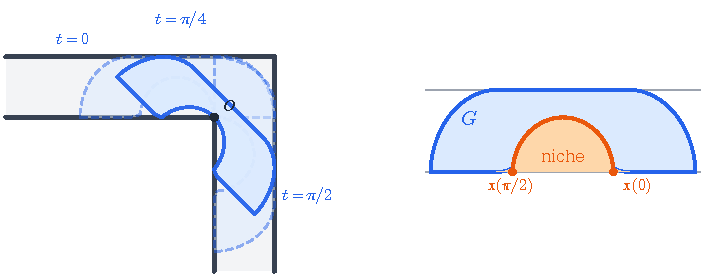
\includegraphics[width=\linewidth]{figures/fig-intro}
\caption{Gerver's sofa $\Gs$ in the hallway $L$. Left: it slides along the horizontal side (dashed), turns
through a right angle around the inner corner (solid, halfway, turned by $\pi/4$) and leaves along the
vertical side (dashed). Right: $\Gs$ with its niche, the hollow in its lower side that makes room for the
corner; the path $\xx$ of the inner corner of the hallway, as seen from the sofa, is drawn in orange.}
\label{fig:intro}
\end{figure}

\subsection{Uniqueness}

We prove that Gerver's sofa is the only optimal sofa, up to a rotation and a translation.

\begin{theorem}[uniqueness of Gerver's sofa]\label{thm:main}
Let $S$ be a moving sofa with $\abs S=\abs\Gs$. Then there are an angle $\theta$ and a vector $v$ such that
\[
  R_\theta S+v=\Gs .
\]
\end{theorem}

Equivalently, a moving sofa has maximum area if and only if it is a rotated and translated copy of $\Gs$
(\cref{cor:all}).

The theorem gives an equality of sets. This uses that a moving sofa is closed and that $\Gs$ is the closure of
its interior (\cref{sec:recovery}); equality of areas alone would determine a set only up to a null set.

The rotation in \cref{thm:main} can be taken to be trivial. The width of $\Gs$ exceeds one in every
direction other than the vertical (\cref{lem:gerver-width}), so a copy $R_\theta\Gs$ is a moving sofa only if $\theta$ is a
multiple of $\pi$. The proof of \cref{thm:main} produces $\theta\in[0,\pi/2-\omega_0]$, so that $\theta=0$ and every
moving sofa of maximal area is a translate of $\Gs$ (\cref{cor:translate}).

Baek's paper does not claim uniqueness. At the time of writing, Google DeepMind's formal-conjectures project
lists the statement as an open problem~\cite{FormalConjectures}, and we know of no earlier proof.

The proof also describes the extremal caps: the caps with rotation angle $\pi/2$ that maximize Baek's sofa area
functional (\cref{sec:sofas}) are the horizontal translates of Gerver's cap (\cref{thm:caps}).

\subsection{Baek's argument and the strategy of the proof}

Baek's proof has four steps.
\begin{enumerate}[label=(\arabic*)]
\item After a translation, a moving sofa lies in a \emph{monotone} sofa, which is a convex body $K$, its
\emph{cap}, minus a \emph{niche} $\cN(K)$ cut out by the inner corners of the supporting hallways. The
problem becomes the maximization of $\cA_\omega(K)=\abs K-\abs{\cN(K)}$ over caps with rotation angle $\omega$.
\item For every $\omega$ he constructs a maximizing cap as a limit of \emph{maximum polygon caps}, which are
\emph{balanced}: each side of the cap is as long as the corresponding side of the niche, since otherwise
pushing one wall of one hallway would increase the area (Gerver's balancing argument).
\item From the balance he shows that, if the area is at least $11/5$, a rotated copy of the sofa
$K\setminus\cN(K)$ of this cap turns through the full right angle, so that only the rotation angle $\pi/2$
matters. From the balance he also shows that for the rotation angle $\pi/2$ the cap satisfies the
\emph{injectivity condition}: the inner corner of the hallway, as seen from the sofa, moves steadily to the left
and never crosses its own path.
\item For caps with the injectivity condition, a concave quadratic functional $\cQ$ bounds the area, and
Gerver's cap maximizes it.
\end{enumerate}

Suppose now that $S$ has area $\abs\Gs$. Every inequality in the chain of Baek's estimates becomes an equality,
but this chain compares $\abs S$ with the areas of other sets, namely its monotonization and Baek's special
balanced maximum sofa. A maximizing cap given in advance need not be a limit of maximum polygon caps, and then the
properties of steps (2) and (3) are known only for the cap that Baek constructed.

We replace the balance by bounds that we prove for every maximizing cap $K_*$ of positive sofa area. We approximate $K_*$ by polygon caps $K_n$
that maximize the polygon sofa area minus a penalty for straying from $K_*$ (\cref{sec:selection}). The penalty
is a weighted sum of squared differences of support values at dyadic normals, with weights that persist from one
approximation to the next and add up to at most $1$. Pushing one side of $K_n$ as in Gerver's balancing argument
shows that $K_n$ is almost balanced: at each normal, the difference between the length $\sigma$ of the side of
the cap and the length $\tau$ of the corresponding side of the niche is at most a multiple of the distance from
$K_n$ to $K_*$ at the sampled normals, and by the choice of the weights these bounds add up to
$O(\dH(K_n,K_*))$ (\cref{sec:variations}).

In the limit this gives two inequalities between wedge gaps and side lengths of $K_*$, the pinned bounds. They
suffice for Baek's rotation argument (\cref{sec:right-angle}), which produces a second monotone sofa $U$ of area
$\abs\Gs$ with rotation angle $\pi/2$ that contains a rigid image of $S$. For the maximizing cap $K$ of $U$, the
same selection gives the curvature bounds $\sigma_{K}\le k_0(g_K^+(t))\dd t$ on $[0,\pi/2)$ and
$\sigma_{K}\le k_0(f_K^-(t-\pi/2))\dd t$ on $(\pi/2,\pi]$, from which the injectivity condition
follows (\cref{sec:injectivity}).

Then $\abs\Gs=\cA(K)\le\cQ(\xi_K)\le\abs\Gs$ is an equality, and equality in $\cQ$ forces equality in each of its
convex Mamikon terms. By Mamikon's theorem, each of these is half the integral of the squared length $\varrho$ of a tangent
segment, $\frac12\int\varrho^2$. Equality in each term gives differential equations for the difference of the support functions of $K$
and of Gerver's cap, whose solutions are $s\cos t$, so that $K$, and with it $U$, is a horizontal translate of
Gerver's cap and sofa (\cref{sec:equality}). Finally $\Gs$ is the closure of its interior, which turns the inclusion of a rigid
image of $S$ in $\Gs$ into an equality (\cref{sec:recovery}).

What is new compared with~\cite{Baek} is \cref{thm:main} and its proof: the penalized selection with persistent
samples, which gives the defect bounds for an arbitrary maximizer; the use of these bounds in place of the
balance in Baek's arguments of his Chapters~4 and~6; the equality case of Baek's bound, with the description of
the extremal caps (\cref{thm:caps}); and the regularity of $\Gs$ that recovers the set. The formalization of
\cref{thm:main} is new. Baek's theorem is also formalized in~\cite{Cureton,Cao}, and twelve findings of the
audit of~\cite{Baek} that accompanies our formalization~\cite{Companion} come from the notes of~\cite{Cureton}.

\subsection{Formal verification and the use of AI}

The proof, together with Baek's, is formalized in Lean~4 with Mathlib~\cite{Lean4,Mathlib20}, in the
repository~\cite{Companion}: every result of~\cite{Baek} used here, with the corrections of
Appendix~\ref{app:corrections}, and the proof of \cref{thm:main}. The statement of \cref{thm:main} is
\path{Baek.gerver_sofa_unique} in \path{Challenge.lean}, and Appendix~\ref{app:lean} lists the Lean declarations
behind each result of this paper. Three of the Facts of \cref{sec:setting}
(\cref{fact:Q}\ref{fact:Q:triple}, \cref{fact:gerver} and \cref{fact:height}) are known to us only through the
formalization.

At the author's request, AI systems wrote the first version of the proof, the formalization and this text.
\cref{sec:formalization} names them, describes what each did, and says what has and has not been checked. Lean's kernel has checked the formalization; the argument has not been peer reviewed, and
no person has checked it independently of the formalization.

\subsection{Organization}

\cref{sec:setting} recalls the definitions and the results of~\cite{Baek} that we use. \cref{sec:reduction}
reduces the theorem to caps and outlines the rest; \cref{sec:selection,sec:variations,sec:right-angle,sec:injectivity,sec:equality,sec:recovery} carry out the strategy described above;
\cref{sec:formalization} describes the formalization and the use of AI, and lists open questions. The appendices give the
explicit description of Gerver's sofa, the corrections to~\cite{Baek}, and the dictionary to the Lean
declarations.

\section{Setting, and what we use from Baek's paper}\label{sec:setting}

This section fixes the notation and records the results that the proof uses and does not prove; we call
them \emph{Facts}. Most are results of Baek's paper~\cite{Baek}, quoted in the form in which we use them
and with the numbering of version~1 of the preprint (chapter.section.number). A few printed statements need a
correction, and a few are used for objects slightly more general than those of their printed statements;
each such place is noted with a label E$n$, the number of the correction in the audit that accompanies the
formalization~\cite{Companion}, and Appendix~\ref{app:corrections} lists them. Some corrections come from
the notes of another formalization of Baek's proof~\cite{Cureton}. Three Facts are known to us only through
the formalization, because the printed proof is missing or invalid, or because the statement is not in~\cite{Baek}: \cref{fact:Q}\ref{fact:Q:triple} (E21),
\cref{fact:gerver} (E12, E24) and \cref{fact:height}; they are proved in~\cite{Companion}, and
\cref{sec:formalization} says what that means. The reader who knows~\cite{Baek} can skim this section and
return to it for the notation.

\subsection{Notation and convex bodies}

The plane is $\R^2$, with points $p=(x,y)$, inner product $\ip pq$ and norm $\norm p$; $\abs X$ is the
area (Lebesgue measure) of $X\subset\R^2$. For an angle $t\in\R$ put
\[
  u_t=(\cos t,\sin t),\qquad v_t=(-\sin t,\cos t)=u_{t+\pi/2},
\]
and let $R_t$ be the counterclockwise rotation by $t$. For $c\in\R$ let
$l(t,c)=\{p:\ip p{u_t}=c\}$, $H_-(t,c)=\{p:\ip p{u_t}\le c\}$, $H_+(t,c)=\{p:\ip p{u_t}\ge c\}$, and let
$H^\circ_\pm$ be the open half-planes. The half-plane $H_-(t,c)$ has \emph{normal angle} $t$.

A \emph{convex body} is a nonempty compact convex subset of $\R^2$; it may be a segment or a point. Its
\emph{support function} is $h_K(t)=\max_{p\in K}\ip p{u_t}$, its \emph{supporting line} is
$l_K(t)=l(t,h_K(t))$, and $H_K(t)=H_-(t,h_K(t))$. Then $K=\bigcap_tH_K(t)$, so $h_K$ determines $K$;
$h_{K+w}(t)=h_K(t)+\ip w{u_t}$ and $h_{(1-\lambda)K+\lambda L}=(1-\lambda)h_K+\lambda h_L$ for
Minkowski combinations. The Hausdorff distance is $\dH(K,L)=\sup_t\abs{h_K(t)-h_L(t)}$, and
$K_n\to K$ means $\dH(K_n,K)\to0$. The \emph{edge} of $K$ with normal angle $t$ is the segment
$e_K(t)=K\cap l_K(t)=[v_K^-(t),v_K^+(t)]$, where $v_K^+(t)$ is its endpoint farthest in the
direction $v_t$; it may be a point. For angles $a,b$ with $\sin(b-a)\ne0$ the supporting lines
$l_K(a)$ and $l_K(b)$ meet at
\[
  v_K(a,b)=h_K(a)\,u_a+\frac{h_K(b)-h_K(a)\cos(b-a)}{\sin(b-a)}\,v_a .
\]

\begin{fact}[convex bodies]\label{fact:convex}
Let $K$ be a convex body.
\begin{enumerate}[label=(\alph*)]
\item\label{fact:convex:vertices} $h_K$ has the one-sided derivatives $h_K'(t^\pm)=\ip{v_K^\pm(t)}{v_t}$;
$v_K^+$ is right-continuous and $v_K^-$ left-continuous; $v_K(t,s)\to v_K^+(t)$ as $s\downarrow t$ and
$v_K(s,t)\to v_K^-(t)$ as $s\uparrow t$. \baek{Thm.~2.1.3}
\item\label{fact:convex:sigma} The \emph{surface area measure} $\sigma_K$ is the Lebesgue--Stieltjes measure
on $\R$ of $G_K(t)=\ip{v_K^+(t)}{v_t}+\int_0^th_K$ (formally $\sigma_K=h_K''+h_K$); it is
$2\pi$-periodic. We write $\sigma_K(t)=\sigma_K(\{t\})$. Its atoms are the edge lengths:
$\sigma_K(t)=\abs{e_K(t)}$ and $v_K^+(t)=v_K^-(t)+\sigma_K(t)v_t$. Moreover
$v_K^+(d)-v_K^+(c)=\int_{(c,d]}v_s\dd\sigma_K(s)$ for $c\le d$, and
$\abs K=\tfrac12\int_{[0,2\pi)}h_K\dd\sigma_K$.
\baek{Prop.~2.1.2, Thm.~5.2.2}, \cite[Rem.~5.1.2]{Schneider14}
\item\label{fact:convex:blaschke} Every sequence of convex bodies in a bounded set has a subsequence that
converges to a convex body (Blaschke's selection theorem), and $K\mapsto\abs K$ is continuous for $\dH$.
\cite[Section~1.8, in particular Thm.~1.8.20]{Schneider14}
\end{enumerate}
\end{fact}

Baek's Thm.~2.1.3 states the limits in \ref{fact:convex:vertices}; the formulas for the one-sided derivatives follow from them and
from $\ip{v_K(t,s)}{v_t}=\bigl(h_K(s)-h_K(t)\cos(s-t)\bigr)/\sin(s-t)$, and the printed statement has a misprint (E27).
From \ref{fact:convex:sigma} one reads off, for $a<b$,
\begin{equation}\label{eq:sigma-open}
  \sigma_K\bigl((a,b)\bigr)=\ip{v_K^-(b)}{v_b}-\ip{v_K^+(a)}{v_a}+\int_a^bh_K .
\end{equation}

\subsection{Moving sofas, monotonization, caps and niches}\label{sec:sofas}

The \emph{hallway} is $L=H_L\cup V_L$, the union of its horizontal side $H_L=(-\infty,1]\times[0,1]$
and its vertical side $V_L=[0,1]\times(-\infty,1]$; its inner corner is the origin $O$ and its outer
corner is $(1,1)$.

\begin{definition}[moving sofa]\label{def:sofa}
A \emph{movement} of a set $S\subset\R^2$ is a pair of continuous maps $\theta:[0,1]\to\R$,
$c:[0,1]\to\R^2$ with $\theta(0)=0$ such that the rigid motions $\Phi_s(p)=R_{\theta(s)}p+c(s)$ satisfy
\[
  \Phi_0(S)\subset H_L,\qquad \Phi_s(S)\subset L\ \ (0\le s\le1),\qquad \Phi_1(S)\subset V_L .
\]
Its \emph{rotation angle} is $\omega=-\theta(1)$. A \emph{moving sofa} is a nonempty, closed and
connected set that has a movement; it is a moving sofa \emph{with rotation angle $\omega$} if it has a
movement with that rotation angle.
\end{definition}

This is \baek{Def.~1.1.2}: Baek moves the set along a continuous curve of orientation-preserving
isometries that starts at a translation, and the angle of such a curve lifts to a continuous real
function. A moving sofa is bounded, hence compact: the start and end positions bound it unless $\theta(1)\in\pi/2+2\pi\mathbb Z$, and then a
position in the middle of the movement does (in Lean, \path{isBounded_of_isMovingSofa}). A translate of a moving sofa with
rotation angle $\omega$ is again one. Let $\omega_0=\sec^{-1}(11/5)=\arccos(5/11)=1.0989\ldots$ ($63^\circ$ approximately).

For $\omega\in(0,\pi/2]$ let $H=\R\times[0,1]$ be the horizontal strip, $V_\omega=\{p:0\le\ip p{u_\omega}\le1\}$,
$P_\omega=H\cap V_\omega$ the parallelogram (a strip if $\omega=\pi/2$), and
$F_\omega=\{p:y\ge0,\ \ip p{u_\omega}\ge0\}$ the \emph{fan}. If $\omega<\pi/2$ the two upper sides of
$P_\omega$ meet at $o_\omega=(c_\omega,1)$, $c_\omega=\sec\omega-\tan\omega$, and the two lower sides at $O$.
A moving sofa $S$ with rotation angle $\omega$ is in \emph{standard position} if $h_S(\omega)=h_S(\pi/2)=1$.

\begin{fact}[rotation angle and standard position]\label{fact:angle}
\begin{enumerate}[label=(\alph*)]
\item Every moving sofa $S$ with $\abs S\ge 11/5$ is a moving sofa with some rotation angle
$\omega\in[\omega_0,\pi/2]$. \baek{Thm.~1.5.1}
\item If $S$ is a moving sofa with rotation angle $\omega\in(0,\pi/2]$, some translate $S+v$ is in
standard position, and a moving sofa with rotation angle $\omega$ in standard position
lies in $P_\omega$. \baek{Prop.~1.2.1, Prop.~2.3.1}
\end{enumerate}
\end{fact}

\runin{Supporting hallways.} For a compact set $S$ and an angle $t$ let
\[
  f_{S,t}(p)=R_tp+(h_S(t)-1)u_t+(h_S(t+\pi/2)-1)v_t ,
\]
and let $L_S(t)=f_{S,t}(L)$ be the \emph{supporting hallway} of $S$ at $t$: the translate of $R_tL$
whose two outer walls $a_S(t)=l_S(t)$ and $c_S(t)=l_S(t+\pi/2)$ are supporting lines of $S$. Its inner
corner and outer corner are
\begin{align*}
  \xx_S(t)&=(h_S(t)-1)u_t+(h_S(t+\pi/2)-1)v_t,\\
  \yy_S(t)&=h_S(t)u_t+h_S(t+\pi/2)v_t=\xx_S(t)+u_t+v_t,
\end{align*}
its inner walls lie on the lines $b_S(t)=l(t,h_S(t)-1)$ and $d_S(t)=l(t+\pi/2,h_S(t+\pi/2)-1)$ (the half-lines
from $\xx_S(t)$ in the directions $-v_t$ and $-u_t$ are $\vec b_S(t)$ and $\vec d_S(t)$), and
\begin{align*}
  L_S(t)&=Q_S^+(t)\setminus Q_S^-(t),\qquad
  Q_S^+(t)=H_S(t)\cap H_S(t+\tfrac\pi2),\\
  Q_S^-(t)&=H^\circ_-(t,h_S(t)-1)\cap H^\circ_-(t+\tfrac\pi2,h_S(t+\tfrac\pi2)-1).
\end{align*}
$Q_S^-(t)$ is the open quarter-plane below the inner corner. A moving sofa in standard position lies in
$L_S(t)$ for every $t\in[0,\omega]$, and the \emph{monotonization} of $S$ is
\[
  \cI(S)=P_\omega\cap\bigcap_{t\in[0,\omega]}L_S(t).
\]
A \emph{monotone sofa} with rotation angle $\omega$ is a set $\cI(S')$ for a moving sofa $S'$ in
standard position with rotation angle $\omega$.

\runin{Caps and niches.} Let $J_\omega=[0,\omega]\cup[\pi/2,\omega+\pi/2]$. A \emph{cap} with
rotation angle $\omega\in(0,\pi/2]$ is a convex body $K$ with
\[
  h_K(\omega)=h_K(\pi/2)=1,\qquad h_K(\omega+\pi)=h_K(3\pi/2)=0,
\]
that is an intersection of closed half-planes with normal angles in $J_\omega\cup\{\omega+\pi,3\pi/2\}$.
The caps with rotation angle $\omega$ form the set $\Kc_\omega$. A cap lies in $P_\omega$ and touches its
four sides; and
\begin{equation}\label{eq:cap-fan}
  K=F_\omega\cap\bigcap_{s\in J_\omega}H_K(s).
\end{equation}
The \emph{niche} of a cap $K$ and its \emph{sofa area} are
\[
  \cN(K)=F_\omega\cap\bigcup_{t\in(0,\omega)}Q_K^-(t),\qquad \cA_\omega(K)=\abs K-\abs{\cN(K)} .
\]
For $S$ in standard position, the \emph{cap} of $S$ is $\cC(S)=P_\omega\cap\bigcap_{t\in[0,\omega]}Q_S^+(t)$.
The reflection $M_\omega(x,y)=(-x\sin\omega+y\cos\omega,\ x\cos\omega+y\sin\omega)$ in the line through
$O$ at the angle $\pi/4+\omega/2$ (the line through $O$ and $o_\omega$ if $\omega<\pi/2$) maps $P_\omega$ and $F_\omega$ to themselves; for $\omega=\pi/2$ it is
$(x,y)\mapsto(-x,y)$. The \emph{mirror image} of a cap $K$ is $K^{\mir}=M_\omega(K)$.

\begin{figure}[ht]
\centering
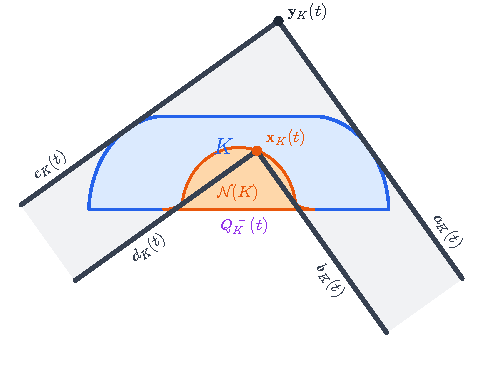
\includegraphics[width=0.74\linewidth]{figures/fig-cap}
\caption{A cap, its niche and a supporting hallway: Gerver's cap $K=\KG$ (blue), its niche $\cN(K)$ (orange), and the
supporting hallway $L_K(t)$ at $t=0.62$ (grey), whose outer walls $a_K(t)$ and $c_K(t)$ touch $K$ and meet at the outer
corner $\yy_K(t)$, and whose inner walls $b_K(t)$ and $d_K(t)$ meet at the inner corner $\xx_K(t)$, on the boundary of the
niche. $Q^-_K(t)$ is the open quarter-plane below the inner corner; the niche is the union of these quarter-planes over
$t\in(0,\pi/2)$, cut at the $x$-axis.}
\label{fig:cap}
\end{figure}

\begin{fact}[monotone sofas and caps]\label{fact:monotone}
Let $\omega\in(0,\pi/2]$.
\begin{enumerate}[label=(\alph*)]
\item\label{fact:monotone:envelope} If $S$ is a moving sofa with rotation angle $\omega$ in standard
position, then $\cI(S)$ is a moving sofa with rotation angle $\omega$ in standard position and
$S\subset\cI(S)$. \baek{Thm.~2.3.2}
\item\label{fact:monotone:cap} For such an $S$, $K=\cC(S)$ is a cap with $h_K=h_S$ on $J_\omega$, and
$\cI(S)=K\setminus\cN(K)$. \baek{Lemma~2.3.5, Thm.~2.4.1, Thm.~2.4.2}
\item\label{fact:monotone:area} If $T$ is a monotone sofa with rotation angle $\omega$ and $K=\cC(T)$,
then $T=K\setminus\cN(K)$, $\cN(K)\subset K$ and $\abs T=\cA_\omega(K)$. \baek{Thm.~2.4.3, Thm.~2.5.9, Thm.~2.5.10}
\item\label{fact:monotone:mirror} If $K$ is a cap, so is $K^{\mir}$, with $h_{K^{\mir}}(t)=h_K(\omega+\pi/2-t)$,
$\cN(K^{\mir})=M_\omega(\cN(K))$, $\cA_\omega(K^{\mir})=\cA_\omega(K)$ and
$\sigma_{K^{\mir}}(E)=\sigma_K(\omega+\pi/2-E)$ for Borel sets $E$. \baek{Prop.~2.5.4}
\end{enumerate}
\end{fact}

Three places need a remark. The proof of \ref{fact:monotone:envelope} uses Def.~2.3.9, which defines the left and the right side of a line
for lines not parallel to the $y$-axis, where it needs the $x$-axis (E1). In \ref{fact:monotone:cap}, the union over $t\in[0,\omega]$ in
Thm.~2.4.2 and the union over $(0,\omega)$ in the definition of the niche agree after intersection with $F_\omega$, and $\cC(S)$ is bounded also for $\omega=\pi/2$, which Baek does not show (E2). In
\ref{fact:monotone:mirror}, Prop.~2.5.4 prints $?_{K^{\mir}}(t)=M_\omega(?_K(\omega-t))$ for each of the walls $a,b,c,d$ and the ends $W,Z$, whereas $M_\omega$
exchanges $a\leftrightarrow c$, $b\leftrightarrow d$ and $W\leftrightarrow Z$, and the identity for the vertices has $K^{\mir}$ in place of $K$ on
the right (E3); \ref{fact:monotone:mirror} uses none of this.

Two more facts about caps are used without proof in Baek's \baek{Lemma~2.5.6}, \baek{Lemma~3.4.8} and \baek{Thm.~2.5.8} (E4): that $O$ and $o_\omega$ lie in every cap if $\omega<\pi/2$
(the statement about $o_\omega$ is not in the audit), and where the ends of the \emph{upper boundary} $\bigcup_{t\in[0,\omega+\pi/2]}e_K(t)$ of a cap $K$ are. Here
$A_K^\pm(t)=v_K^\pm(t)$ and $C_K^\pm(t)=v_K^\pm(t+\pi/2)$ \baek{Def.~2.5.1, Def.~2.5.2}.

\begin{lemma}[every cap contains $O$ and $o_\omega$]\label{lem:contains}
If $\omega<\pi/2$, every cap $K\in\Kc_\omega$ contains $O$ and $o_\omega$; in particular $h_K\ge0$. For $\omega=\pi/2$ the origin need not lie in $K$ (take $K=[5,6]\times[0,1]$).
\end{lemma}

\begin{proof}
Let $q\in K\cap l(\pi/2,1)$ and $q'\in K\cap l(\omega,1)$. As $K\subset P_\omega$, $q=o_\omega-\lambda u_0$ and $q'=o_\omega-\mu v_\omega$ with $\lambda,\mu\ge0$.
For $s\in[0,\omega]$, $\ip{o_\omega}{u_s}=\ip{q'}{u_s}+\mu\sin(s-\omega)\le\ip{q'}{u_s}\le h_K(s)$, and for $s\in[\pi/2,\omega+\pi/2]$,
$\ip{o_\omega}{u_s}=\ip q{u_s}+\lambda\cos s\le\ip q{u_s}\le h_K(s)$. As $o_\omega\in F_\omega$, \eqref{eq:cap-fan} gives $o_\omega\in K$. Then $h_K(s)\ge\ip{o_\omega}{u_s}=c_\omega\cos s+\sin s=\sqrt{1+c_\omega^2}\,\sin\bigl(s+\tfrac\pi4-\tfrac\omega2\bigr)$, because
$c_\omega=\tan(\pi/4-\omega/2)$, and $0<s+\pi/4-\omega/2<\pi$ for $s\in J_\omega$, so $h_K\ge0$ on $J_\omega$. Hence $O\in F_\omega$ satisfies $\ip O{u_s}=0\le h_K(s)$ for
$s\in J_\omega$, and $O\in K$ by \eqref{eq:cap-fan}; and $h_K(s)\ge\ip O{u_s}=0$ for every $s$.
\end{proof}

\begin{lemma}[the ends of the upper boundary]\label{lem:ends}
For every cap $K\in\Kc_\omega$,
\begin{equation}\label{eq:ends}
  A_K^-(0)=(h_K(0),0)\quad\text{and}\quad C_K^+(\omega)=h_K(\omega+\pi/2)\,v_\omega ;
\end{equation}
they lie on $l(\pi/2,0)$ and on $l(\omega,0)$.
\end{lemma}

\begin{proof}
Let $q\in e_K(\omega+\pi/2)$ and $p=q-\ip q{u_\omega}u_\omega=h_K(\omega+\pi/2)v_\omega$. Since $\ip q{u_\omega}\ge0$ ($K\subset P_\omega$) and $\cos(s-\omega)\ge0$ for $s\in J_\omega$, we have
$\ip p{u_s}\le\ip q{u_s}\le h_K(s)$ for $s\in J_\omega$. Also $p\in F_\omega$, since $h_K(\omega+\pi/2)\ge0$ (\cref{lem:contains}; for $\omega=\pi/2$, $p_y=0$). So $p\in K$ by \eqref{eq:cap-fan}.
As $\ip\cdot{u_\omega}\ge0=\ip p{u_\omega}$ on $K$, $p$ is the point of $e_K(\omega+\pi/2)$ farthest in the direction $v_{\omega+\pi/2}=-u_\omega$, that is $p=C_K^+(\omega)$.
The mirror image $K^{\mir}$ is a cap (\cref{fact:monotone}\ref{fact:monotone:mirror}) with $h_{K^{\mir}}(\omega+\pi/2)=h_K(0)$, and $M_\omega$ maps $v_\omega$ to $u_0$ and reverses orientation, so that
$C^+_{K^{\mir}}(\omega)=h_K(0)v_\omega$ is mapped to the lower end $A_K^-(0)$ of $e_K(0)$, which is $(h_K(0),0)$.
\end{proof}

The next fact is the main theorem of \cite{Baek}, in the form for caps. It assembles Baek's
construction of a balanced maximum cap $K_\omega$ for every $\omega$ (\baek{Thm.~3.5.2, Thm.~3.5.4}), its
maximality (\baek{Thm.~3.5.5}), and the optimality of Gerver's sofa $\Gs$ (\baek{Thm.~1.1.1}), which is
recalled in \cref{sec:gerver}.

\begin{fact}[optimality]\label{fact:optimal}
Every moving sofa $S$ has $\abs S\le\abs\Gs$, and $\abs\Gs>11/5$. For every $\omega\in(0,\pi/2]$ and every
cap $K\in\Kc_\omega$, $\cA_\omega(K)\le\abs\Gs$.
\end{fact}

For the last claim, \baek{Thm.~3.5.6} gives a monotone sofa $S_\omega=K_\omega\setminus\cN(K_\omega)$ whose cap
$K_\omega$ satisfies $\cA_\omega(K)\le\cA_\omega(K_\omega)$ for every cap $K$ \baek{Thm.~3.5.5}, and
$\cA_\omega(K_\omega)=\abs{S_\omega}\le\abs\Gs$ by \baek{Thm.~1.1.1} and \cref{fact:monotone}\ref{fact:monotone:area}.

\subsection{Polygon caps}\label{sec:polygon}

Let $\omega\in(0,\pi/2]$. An \emph{angle set} is a finite nonempty $\Theta\subset(0,\omega)$, and
$\Theta^\diamond=\Theta\cup(\Theta+\pi/2)\cup\{\omega,\pi/2\}\subset(0,\pi)$ is its set of
\emph{defining normals}; the two normals $\omega$ and $\pi/2$, which carry the two strips of $P_\omega$,
are \emph{pinned}, the others \emph{floating}. A \emph{polygon cap} with angle set $\Theta$ is a cap
that is an intersection of closed half-planes with normal angles in
$\Theta^\diamond\cup\{\omega+\pi,3\pi/2\}$; they form the set $\Kc_\Theta\subset\Kc_\omega$. A polygon cap
is the intersection of its supporting half-planes $H_K(s)$ at these normal angles. For a cap $K$ put
\begin{align*}
  \cC_\Theta(K)&=P_\omega\cap\bigcap_{t\in\Theta}Q_K^+(t),\qquad
  \cN_\Theta(K)=F_\omega\cap\bigcup_{t\in\Theta}Q_K^-(t),\\
  \cA_\Theta(K)&=\abs{\cC_\Theta(K)}-\abs{\cN_\Theta(K)} .
\end{align*}
Here the \emph{fan} $F_\omega$, and not the parallelogram $P_\omega$, cuts the polygon niche: the
printed \baek{Def.~3.2.5} has $P_\omega$ and with it \baek{Prop.~3.3.5} and \baek{Lemma~3.4.2} are
false, whereas the results of \baek{Ch.~3} hold with $F_\omega$, as the formalization proves (E6).

\begin{fact}[the polygon bound]\label{fact:polygon}
For every cap $K$ and angle set $\Theta$, $\cC_\Theta(K)$ is a polygon cap that contains $K$ and has the
same support values as $K$ on $\Theta^\diamond$, and $\cC_\Theta(K)=K$ if $K\in\Kc_\Theta$;
$\cN_\Theta(K)=\cN_\Theta(\cC_\Theta(K))\subset\cN(K)$. Hence
$\cA_\omega(K)\le\cA_\Theta(K)=\cA_\Theta(\cC_\Theta(K))$, and $\cA_\Theta(K)=\abs K-\abs{\cN_\Theta(K)}$
for a polygon cap. \baek{Prop.~3.2.1, Prop.~3.2.2, Thm.~3.2.3}
\end{fact}

\begin{fact}[bounded width]\label{fact:width}
For $t\in(0,\omega)$ there is a constant $c_{\omega,t}$ such that every polygon cap $K$ with an angle set $\Theta\ni t$
and $\cA_\Theta(K)>0$ has width $h_K(0)+h_K(\pi)\le c_{\omega,t}$. \baek{Lemma~3.4.2}
\end{fact}

\runin{Sides of the polygon niche.} For a polygon cap $K$ with angle set $\Theta$, the boundary of
$F_\omega\setminus\cN_\Theta(K)$ consists of an open half-line, a polyline $\mathbf p_K$ from
$C_K^+(\omega)$ to $A_K^-(0)$ (see \eqref{eq:ends}), along which the abscissa increases and whose segments have normal angles in $\Theta^\diamond$,
and an open half-line \baek{Thm.~3.4.4}.
For $t\in\Theta^\diamond$ let $\tau_K(t)$ be the total length of the segments of $\mathbf p_K$ with normal
angle $t$, and $\sigma_K(t)=\abs{e_K(t)}$ the length of the edge of $K$ with normal angle $t$.
The following is about every polygon cap; maximality plays no role in it.

\begin{fact}[sides of the polygon niche]\label{fact:sides}
Let $K\in\Kc_\Theta$.
\begin{enumerate}[label=(\alph*)]
\item\label{fact:sides:wall} For $t\in\Theta$, $\Hone(\partial\cN_\Theta(K)\cap\vec b_K(t))=\tau_K(t)$ and
$\Hone(\partial\cN_\Theta(K)\cap\vec d_K(t))=\tau_K(t+\pi/2)$. \baek{Lemma~3.4.5\,(1)}
\item\label{fact:sides:floor} For $t\in\{\omega,\pi/2\}$, $\Hone(\cN_\Theta(K)\cap l(t,0))=\sigma_K(t+\pi)-\tau_K(t)$.
\baek{Lemma~3.4.5\,(2)}
\item\label{fact:sides:identity}
$\displaystyle\sum_{t\in\Theta^\diamond}\sin t\,\bigl(\sigma_K(t)-\tau_K(t)\bigr)=0$. \baek{Proof of Lemma~3.4.6}
\end{enumerate}
\end{fact}

Baek obtains \ref{fact:sides:identity} from the vector identity $\sum_t\tau_K(t)v_t=C_K^+(\omega)-A_K^-(0)=\sum_t\sigma_K(t)v_t$, by taking the inner product with $u_0$
(note $\ip{v_t}{u_0}=-\sin t$); the formalization proves \ref{fact:sides:identity} in this sine form, and of the vector identity only its $\sigma$ half.

\runin{Support values and first variations.} For $h:\Theta^\diamond\to\R$ let
\begin{align*}
  P_h&=\bigcap_{s\in\{\omega,\pi/2\}}\bigl(H_-(s,h(s))\cap H_+(s,h(s)-1)\bigr),\\
  \cC_\Theta(h)&=P_h\cap\bigcap_{s\in\Theta^\diamond\setminus\{\omega,\pi/2\}}H_-(s,h(s)),\\
  F_h&=\bigcap_{s\in\{\omega,\pi/2\}}H_+(s,h(s)-1),\\
  \cN_\Theta(h)&=F_h\cap\bigcup_{t\in\Theta}\bigl(H^\circ_-(t,h(t)-1)\cap H^\circ_-(t+\tfrac\pi2,h(t+\tfrac\pi2)-1)\bigr),
\end{align*}
and $\cA_\Theta(h)=\abs{\cC_\Theta(h)}-\abs{\cN_\Theta(h)}$ (\baek{Def.~3.3.3}). For a polygon cap $K$ and
$h=h_K|_{\Theta^\diamond}$ these are $K$, $\cN_\Theta(K)$ and $\cA_\Theta(K)$ (\baek{Prop.~3.3.4, Prop.~3.3.5}, with $F_\omega$, E6). For $\eps>0$ and
$t\in\Theta^\diamond$ let $h^{t,\eps}_K$ be $h_K$ with the value at $t$ replaced by $h_K(t)+\eps$.

\begin{fact}[pushing one side]\label{fact:push}
Let $K\in\Kc_\Theta$ and $t\in\Theta^\diamond$.
\begin{enumerate}[label=(\alph*)]
\item\label{fact:push:derivative} There are $\eps_0>0$ and $M\ge0$ such that for $0<\eps\le\eps_0$
\[
  \bigl\lvert\cA_\Theta(h^{t,\eps}_K)-\cA_\Theta(K)-(\sigma_K(t)-\tau_K(t))\eps\bigr\rvert\le M\eps^2 .
\]
\item\label{fact:push:translate} If $\sigma_K(t)>0$, then for small $\eps>0$ the set $\cC_\Theta(h^{t,\eps}_K)$ is a translate $C+v$
of a polygon cap $C\in\Kc_\Theta$.
\item\label{fact:push:area} If $\cC_\Theta(h^{t,\eps}_K)=C+v$ with $C\in\Kc_\Theta$, then $\cA_\Theta(h^{t,\eps}_K)\le\cA_\Theta(C)$.
\end{enumerate}
\baek{Lemma~3.4.7, Lemma~3.4.8, Prop.~3.3.7, Thm.~3.3.6}
\end{fact}

Part \ref{fact:push:derivative} rests on \baek{Thm.~3.1.2}, which needs the Nef polygon (a set obtained from finitely many half-planes by intersections, unions and
complements) to be bounded; every use is to bounded polygons (E5, and Section~4 of REPORT.md in~\cite{Companion}). In the proof of
\baek{Lemma~3.4.7} the sign of the change of $\abs{\cN_\Theta}$ is misprinted (E27).

\subsection{The injectivity condition and arm lengths}\label{sec:arms}

The rest of this section, and \cref{sec:injectivity,sec:equality}, concern caps with rotation angle $\pi/2$, and
$\cA=\cA_{\pi/2}$. For $K\in\Kc_{\pi/2}$ the \emph{arm lengths} are
\[
  f_K^\pm(t)=\ip{\yy_K(t)-A_K^\pm(t)}{v_t},\qquad g_K^\pm(t)=\ip{\yy_K(t)-C_K^\pm(t)}{u_t},
\]
with $\yy_K(t)=h_K(t)u_t+h_K(t+\pi/2)v_t$ the outer corner of the supporting hallway and
$A_K^\pm,C_K^\pm$ as in \eqref{eq:ends}. Thus $\yy_K(t)=A_K^\pm(t)+f_K^\pm(t)v_t=C_K^\pm(t)+g_K^\pm(t)u_t$: these are
the distances from the outer corner to the points where $K$ touches the two outer walls. They are
nonnegative, $g_K^-\le g_K^+$, and $f_K^\pm,g_K^\pm$ are at most the diameter of $K$, because
$A_K^\pm(t)-C_K^\pm(t)=g_K^\pm(t)u_t-f_K^\pm(t)v_t$ joins two points of $K$.

\begin{definition}[injectivity condition]\label{def:inj}
A cap $K\in\Kc_{\pi/2}$ satisfies the \emph{injectivity condition} if
\begin{enumerate}[label=(\arabic*),leftmargin=2.2em]
\item $\sigma_K$ has a density on $[0,\pi/2)$ and on $(\pi/2,\pi]$ (the top edge, at $\pi/2$, may carry an atom);
\item the inner corner $\xx_K$ is continuously differentiable on $[0,\pi/2]$;
\item $\ip{\xx_K'(t)}{u_t}<0<\ip{\xx_K'(t)}{v_t}$ for $0<t<\pi/2$.
\end{enumerate}
We write $\Ki$ for the set of caps in $\Kc_{\pi/2}$ that satisfy the injectivity condition and have
$\abs K\ge11/5$.
\end{definition}

Condition (3) implies that the inner corner moves strictly to the left, so the path of the inner corner has
no self-intersections. We use the following.

\begin{fact}[arms]\label{fact:arms}
Let $K\in\Kc_{\pi/2}$.
\begin{enumerate}[label=(\alph*)]
\item\label{fact:arms:deriv} For every $t$, $\xx_K$ has the right derivative
$-(f_K^+(t)-1)u_t+(g_K^+(t)-1)v_t$, and the left derivative given by the same formula with $f^-_K,g^-_K$.
\baek{Thm.~6.2.3}
\item\label{fact:arms:integral} $f_K^+(b)-f_K^+(a)=\int_a^bg_K^+-\sigma_K((a,b])$ for $0\le a\le b\le\pi/2$.
\baek{Thm.~6.2.5}
\item\label{fact:arms:mirror} For the reflection $K^{\mir}$ in $x\mapsto-x$, $f_{K^{\mir}}^\pm(t)=g_K^\mp(\pi/2-t)$ and
$g_{K^{\mir}}^\pm(t)=f_K^\mp(\pi/2-t)$. \baek{Prop.~6.2.2}
\item\label{fact:arms:regular} If $K$ satisfies (1), then $A_K^+=A_K^-$ and $f_K^+=f_K^-$ on $[0,\pi/2)$,
$C_K^+=C_K^-$ and $g_K^+=g_K^-$ on $(0,\pi/2]$. With $A_K=A_K^-$, $C_K=C_K^+$, $f_K=f_K^-$ and $g_K=g_K^+$ these four functions are continuous on
$[0,\pi/2]$; $f_K(0)=g_K(\pi/2)=1$, and $\xx_K'(t)=-(f_K(t)-1)u_t+(g_K(t)-1)v_t$. In particular (2) holds, and
(3) says that $f_K,g_K>1$ on $(0,\pi/2)$. \baek{Def.~6.4.1, Prop.~6.4.5, Prop.~6.4.6} The end values $f_K(0)=g_K(\pi/2)=1$ are not stated there (E17).
\end{enumerate}
\end{fact}

In \ref{fact:arms:mirror} the printed statement forgets that the reflection reverses the angle (E13); in \ref{fact:arms:deriv} the right derivative is called the left one, and the second display of the printed theorem is about the left derivative (E14).
Let
\[
  k_0(x)=\max\Bigl(\abs{x-1},\tfrac{\abs{x-1}+1}2\Bigr),\qquad m_0(x)=x-k_0(x) .
\]
The function $k_0$ is $1$-Lipschitz, and $m_0$ is nondecreasing, with $m_0(x)=\frac32x-1$ on $[0,1]$,
$m_0(x)=\frac x2$ on $[1,2]$ and $m_0(x)=1$ on $[2,\infty)$. For a continuous $f$ on $[0,\pi/2]$ let
$\mathcal Ff(x)=1+\int_0^xm_0(f(\pi/2-u))\dd u$, and let $f_0=0$, $f_{j+1}=\max(f_j,\mathcal Ff_j)$.

\begin{fact}[convergence of arms and the iteration]\label{fact:iteration}
\begin{enumerate}[label=(\alph*)]
\item\label{fact:iteration:arms} If polygon caps $K_n$ with rotation angle $\pi/2$ converge in $\dH$ to a cap $K\in\Kc_{\pi/2}$, then
$\int_0^{\pi/2}\abs{g_{K_n}^+-g_K^+}\to0$. \baek{Lemma~6.4.2}
\item\label{fact:iteration:eleven} $f_{11}(x)>1$ for $x\in(0,\pi/2]$. \baek{Lemma~6.5.5}, which is printed for $x\in(0,1]$ and used on $(0,\pi/2]$ (E17)
\end{enumerate}
\end{fact}

\subsection{Baek's upper bound}\label{sec:Q}

Let $\varphi=\varphi_G=0.03917\ldots$ be Gerver's angle (\cref{sec:gerver}), $\varphi^{\mathrm R}=\varphi$ and
$\varphi^{\mathrm L}=\pi/2-\varphi$. For $K\in\Kc_{\pi/2}$ let $H^{\mathrm b}_K(t)=\{\ip p{u_t}\ge h_K(t)-1\}$ and
$H^{\mathrm d}_K(t)=\{\ip p{v_t}\ge h_K(t+\pi/2)-1\}$ be the closed half-planes bounded by the inner walls $b_K(t)$ and $d_K(t)$, on
the side away from $Q^-_K(t)$, and
\[
  B_K=K\cap\bigcap_{t\in[\varphi^{\mathrm R},\pi/2]}H^{\mathrm b}_K(t),\qquad
  D_K=K\cap\bigcap_{t\in[0,\varphi^{\mathrm L}]}H^{\mathrm d}_K(t).
\]
Baek's upper bound is the functional $\cQ$ of \baek{Def.~8.2.2} on the set $\cT$ of triples $(K,B,D)$ of convex bodies with
$K\in\Ki$, $B,D\subset K$, $h_K(t)+h_B(\pi+t)\le1$ on $[\varphi^{\mathrm R},\pi/2]$ with equality at the
ends, and $h_K(\pi/2+t)+h_D(3\pi/2+t)\le1$ on $[0,\varphi^{\mathrm L}]$ with equality at the ends. The sets $\Ki$ and $\cT$ are closed under Minkowski combinations
$c_\lambda((K,B,D),(K',B',D'))=((1-\lambda)K+\lambda K',\dots)$. A functional on such a set is
\emph{convex-linear} if it commutes with $c_\lambda$, and \emph{convex} or \emph{concave} if it satisfies the
corresponding inequality for $c_\lambda$. The \emph{canonical triple} of $K\in\Ki$ is $\xi_K=(K,B_K,D_K)$.
For a convex body $K$, $a<b<a+\pi$, and a continuous curve $\mathbf z:[a,b]\to\R^2$ of bounded variation
with $\mathbf z(t)\in l_K(t)$, put
\[
  \varrho_{K,\mathbf z}(t)=\ip{\mathbf z(t)-v_K^+(t)}{v_t},\qquad
  \cM_K(a,b;\mathbf z)=\tfrac12\int_a^b\varrho_{K,\mathbf z}(t)^2\dd t .
\]
By Mamikon's theorem \baek{Thm.~7.4.1} (see \cite{Mnatsakanian97}), $\cM_K(a,b;\mathbf z)$ is the area
swept by the tangent segments from $v_K^+(t)$ to $\mathbf z(t)$; we use it only through the formula, which makes $\cM_K(a,b;\mathbf z)$ a convex function of $\varrho_{K,\mathbf z}$.
The curves that occur are the outer corner $\yy_K$ and the tangent line parametrizations
$\mathbf l_K^T(t)=v_K(t,T)$ for $T-\pi<t<T$ (the point where $l_K(t)$ meets $l_K(T)$) and $\mathbf l_K^T(T)=v_K^-(T)$.
Let $\cS_K,\cR_B,\cL_D$ be the \emph{Mamikon terms}
\begin{align*}
  \cS_K&=\cM_K(0,\varphi^{\mathrm R};\mathbf l_K^{\pi/2})+\cM_K(\varphi^{\mathrm R},\varphi^{\mathrm L};\yy_K)\\
  &\qquad+\cM_K(\varphi^{\mathrm L},\tfrac\pi2;\mathbf l_K^{\pi-\varphi})+\cM_K(\tfrac\pi2,\pi;\mathbf l_K^{\pi}),\\
  \cR_B&=\cM_B(\pi+\varphi^{\mathrm R},\tfrac{3\pi}2;\mathbf l_B^{3\pi/2}),\qquad
  \cL_D=\cM_D(\tfrac{3\pi}2,\tfrac{3\pi}2+\varphi^{\mathrm L};\mathbf l_D^{3\pi/2+\varphi^{\mathrm L}}).
\end{align*}
(In the third term $\pi/2+\varphi^{\mathrm L}=\pi-\varphi$.) The printed $\cR_B$ has $\pi/2+\varphi^{\mathrm R}$ in place of
$\pi+\varphi^{\mathrm R}$ (E27).

\begin{fact}[the upper bound]\label{fact:Q}
There is a functional $\cQ$ on $\cT$ such that:
\begin{enumerate}[label=(\alph*)]
\item\label{fact:Q:triple} $\xi_K\in\cT$ for $K\in\Ki$, and $\cA(K)\le\cQ(\xi_K)$. \baek{Thm.~8.1.8, Thm.~8.2.4}
\item\label{fact:Q:decomp} $\cQ(K,B,D)=\Lambda(K)-\cS_K-\cR_B-\cL_D$, where $\Lambda$ (Baek's $\cP_K+\cS_K$, \baek{Def.~8.3.4}) is
convex-linear on $\Ki$. For each of the four terms of $\cS_K$ (resp.\ for $\cR_B$, for $\cL_D$) the
curve $\mathbf z$ above is convex-linear in $K$ (resp.\ in $B$, in $D$), so that $\varrho(t)$ is convex-linear for every $t$, and each of the terms $\cM$, being $\frac12\int\varrho^2$,
is convex. \baek{Lemma~8.3.3, Lemma~8.3.4, Lemma~8.3.7, Thm.~8.3.1, Thm.~8.3.2, Thm.~7.1.2, Thm.~7.4.1}
\item\label{fact:Q:max} $\cQ\le\cQ(\xi_G)=\abs\Gs$ on $\cT$, where $\xi_G=\xi_{\KG}$ is the canonical triple of Gerver's cap.
\baek{Cor.~8.5.8, Thm.~8.4.6}
\end{enumerate}
\end{fact}

Part \ref{fact:Q:triple} is stated in \cite{Baek} with a proof that uses $\cN(K)\subset K$, which $\Ki$ does not
provide; the statement is true and has a proof that avoids it, which is in~\cite{Companion} (E21). Also \baek{Thm.~8.1.1} (convexity of $\Ki$) uses
the Brunn--Minkowski inequality, and it holds as stated.

\subsection{Gerver's sofa}\label{sec:gerver}

Seen from a sofa that turns clockwise by $t\in[0,\pi/2]$, the hallway occupies $\xx(t)+R_tL$; the curve
$\xx:[0,\pi/2]\to\R^2$ is the \emph{rotation path}. The largest set that moves along $\xx$ is its
\emph{shape}
\[
  \operatorname{shape}(\xx)=H_L\cap\bigcap_{t\in[0,\pi/2]}\bigl(\xx(t)+R_tL\bigr)\cap\bigl(\xx(\pi/2)+R_{\pi/2}V_L\bigr).
\]
\emph{Gerver's sofa} $\Gs$ is the shape of Romik's rotation path~\cite{Romik18}, which is glued from five
explicit curves, on $[0,\varphi],[\varphi,\theta],[\theta,\pi/2-\theta],[\pi/2-\theta,\pi/2-\varphi]$ and
$[\pi/2-\varphi,\pi/2]$, with $\varphi=0.03917\ldots$ and $\theta=0.68130\ldots$ (the formulas and Romik's equations
are in Appendix~\ref{app:gerver}). Write $t_0,\dots,t_5=0,\varphi,\theta,\pi/2-\theta,\pi/2-\varphi,\pi/2$,
$\alpha=\ip{\xx'}{u_t}$, $\beta=\ip{\xx'}{v_t}$, and
\[
  \bA=\xx+\alpha v_t+u_t,\quad \bB=\xx+\alpha v_t,\quad \bC=\xx-\beta u_t+v_t,\quad \bD=\xx-\beta u_t
\]
for the contact points of the sofa with the walls of the hallway.

\begin{fact}[Gerver's sofa]\label{fact:gerver}
\begin{enumerate}[label=(\alph*)]
\item\label{fact:gerver:def} Romik's equations have exactly one solution with $\varphi\in[0.039,0.04]$,
$\theta\in[0.68,0.69]$, so $\Gs$ is well defined, and $2.2192\le\abs\Gs\le2.2199$. (Romik asserts, without proof, the uniqueness for $0<\varphi<\theta<\pi/4$; uniqueness in this box
is proved in~\cite{Companion}.)
\item\label{fact:gerver:cap} $\Gs$ is a monotone sofa with rotation angle $\pi/2$. Its cap $\KG=\cC(\Gs)$
satisfies $\Gs=\KG\setminus\cN(\KG)$ and has $A_{\KG}=\bA$, $C_{\KG}=\bC$ and $\xx_{\KG}=\xx$ on $[0,\pi/2]$; and
$\KG$ satisfies the injectivity condition; as $\abs\KG\ge\abs\Gs>11/5$, $\KG\in\Ki$. \baek{Thm.~8.4.1\,(1), Thm.~6.1.2}
\item\label{fact:gerver:niche} Let $\Gamma=\bD([t_0,t_2])\cup\xx([t_1,t_4])\cup\bB([t_3,t_5])$. Then
$\bD(t_0)$ and $\bB(t_5)$ lie on the $x$-axis, $\bD(t_2)=\xx(t_4)$, $\bB(t_3)=\xx(t_1)$, the abscissa is
strictly increasing along $\bD$ and $\bB$ and strictly decreasing along $\xx$ on $(0,\pi/2)$,
at every point of $[t_0,t_1]$ and of $[t_1,t_2]$ the curve $\bD$ has a derivative within that interval that is a positive multiple of $u_t$, and at every point of $[t_3,t_4]$ and of $[t_4,t_5]$ the curve $\bB$ has a
derivative within that interval that is a negative multiple of $v_t$ (the derivatives are one-sided at the ends of the pieces, and jump at $t_1$ and $t_4$), and
\[
  \cN(\KG)=\{q:\ q_y\ge0,\ q_y<\gamma_y\text{ for some }\gamma\in\Gamma\text{ with }\gamma_x=q_x\}.
\]
\baek{Thm.~8.4.1\,(2)--(4)}
\end{enumerate}
\end{fact}

Baek states \baek{Thm.~8.4.1} without proof (his Remark~8.4.1: the properties are ``easy to verify
numerically''), and proves \baek{Thm.~6.1.2} by a misreading of a theorem of Gerver (E12, E24). Both
statements are true; the formalization proves them from Romik's equations by interval
arithmetic~\cite{Companion}. Baek's \baek{Thm.~8.4.1\,(2)} describes the niche as the region enclosed by $\bB$ reversed, $\xx|_{[t_1,t_4]}$, $\bD$ reversed and the segment of
the $x$-axis from $\bD(t_0)$ to $\bB(t_5)$. That open region omits the open segment of the $x$-axis between $\bD(t_0)$ and $\bB(t_5)$, which lies in $\cN(\KG)$ because $F_{\pi/2}$ is closed. Because of the monotonicity of the abscissa,
$\cN(\KG)$ is the set of points of the closed upper half-plane that lie strictly below the curve $\Gamma$, which is the identity in \ref{fact:gerver:niche}; this exact form is proved in~\cite{Companion}. We also use one
numerical fact that is not in~\cite{Baek}:

\begin{fact}[height of the rotation path]\label{fact:height}
$\xx(t)_y<1$ for every $t\in[0,\pi/2]$, and $\xx(t)_y>0$ for $t\in[t_1,t_4]$. In fact $\max_t\xx(t)_y=\xx(\pi/4)_y=0.66426\ldots$ and
$\xx(t_1)_y=\xx(t_4)_y=0.05518\ldots$, but we use only the two bounds, which the formalization proves by interval
arithmetic~\cite{Companion}: $\xx(t)_y\le0.9925$ on each phase, and $\xx_y>0$ on $[t_1,t_4]$.
\end{fact}

\section{From a maximal sofa to a maximizing cap}\label{sec:reduction}

Throughout this section $S$ is a moving sofa with $\abs S=\abs\Gs$. We reduce
the problem to caps and then outline the rest of the proof.

\begin{definition}[maximizing cap]\label{def:maximizing}
Let $\omega\in(0,\pi/2]$. A cap $K\in\Kc_\omega$ is \emph{maximizing} if
$\cA_\omega(C)\le\cA_\omega(K)$ for every $C\in\Kc_\omega$.
\end{definition}

By \cref{fact:optimal}, every cap with $\cA_\omega(K)=\abs\Gs$ is maximizing. A
maximizing cap maximizes $\cA_\omega$ over all caps, including those that do not
contain their niche. Baek obtains a particular maximizing cap, a limit of
maximum polygon caps (\cref{fact:exists}). A given maximizing cap need not be
such a limit.

\begin{proposition}[the monotonization of a maximal sofa]\label{prop:reduction}
Let $S'$ be a moving sofa with rotation angle $\omega\in(0,\pi/2]$ and
$\abs{S'}=\abs\Gs$. Then there are $w\in\R^2$ and a monotone sofa $T$ with
rotation angle $\omega$ such that
\[
  S'+w\subset T,\qquad \abs{T}=\abs\Gs,
\]
and the cap $K=\cC(T)$ is a maximizing cap, with $T=K\setminus\cN(K)$ and
$\cA_\omega(K)=\abs\Gs$. In particular, if $S$ is any moving sofa with $\abs
S=\abs\Gs$, there is such a $T$ for $S'=S$ and some $\omega\in[\omega_0,\pi/2]$.
\end{proposition}

\begin{proof}
By \cref{fact:angle}(b), $S'+w$ is in standard position for some $w$, and is a
moving sofa with rotation angle $\omega$. By
\cref{fact:monotone}\ref{fact:monotone:envelope}, $T=\cI(S'+w)$ is a moving sofa
in standard position containing $S'+w$, and it is a monotone sofa. So
$\abs\Gs=\abs{S'+w}\le\abs{T}\le\abs\Gs$ by \cref{fact:optimal}. By
\cref{fact:monotone}\ref{fact:monotone:cap}, $K=\cC(T)$ is a cap, and
\cref{fact:monotone}\ref{fact:monotone:area} gives $T=K\setminus\cN(K)$ and
$\cA_\omega(K)=\abs{T}=\abs\Gs$; $K$ is maximizing by \cref{fact:optimal}.
Finally, if $\abs S=\abs\Gs$ then $\abs S>11/5$, so $S$ has a rotation angle
$\omega\in[\omega_0,\pi/2]$ by \cref{fact:angle}(a).
\end{proof}

So the problem is to show that $S$ is a rigid image of $\Gs$. The proof follows
$S$ through a chain of sets, each of which contains a rigid image of $S$ and has
area $\abs\Gs$ (\cref{fig:chain}). Steps (1) and (2) are used twice: first for
the maximizing cap $K$ of \cref{prop:reduction}, which has the rotation angle
$\omega$, to obtain step (3), and then, after step (3), for the maximizing cap
of the new monotone sofa $U$ and for its mirror image, which have the rotation
angle $\pi/2$, to obtain step (4).
\begin{enumerate}[label=(\arabic*)]
\item \emph{Selection} (\cref{sec:selection}). A given maximizing cap $K_*$ with
$\cA_\omega(K_*)>0$ is the Hausdorff limit of polygon caps $K_n$ that maximize
the polygon sofa area minus a penalty for straying from $K_*$.
\item \emph{Variations} (\cref{sec:variations}). Pushing one side of $K_n$ shows
that $K_n$ is almost balanced: the defect $\sigma_{K_n}-\tau_{K_n}$ at a normal
is bounded by a multiple of the distance from $K_n$ to $K_*$ at the sampled
normals, and the weights are chosen so that these bounds add up.
\item \emph{The right angle} (\cref{sec:right-angle}). If $\omega<\pi/2$, the
limit of the defect bounds gives the two \emph{pinned bounds}
$w^\circ_{K_*}\le\sigma_{K_*}(\pi/2)$ and $z^\circ_{K_*}\le\sigma_{K_*}(\omega)$
between wedge gaps and side lengths of $K_*$. They give $T$ width at most one in
the directions $u_t$, $t\in[\omega,\pi/2]$, so that a rotated copy $R_\psi T$,
$\psi=\pi/2-\omega$, turns by $\pi/2$. Monotonizing $R_\psi T$ gives a monotone
sofa $U$ with rotation angle $\pi/2$ and $\abs U=\abs\Gs$ that contains a rigid
image of $S$.
\item \emph{Injectivity} (\cref{sec:injectivity}). For the cap $K$ of $U$, the
defect bounds become the curvature bounds $\sigma_K\le k_0(g_K^+(t))\dd t$ on
$[0,\pi/2)$ and $\sigma_K\le k_0(f_K^-(t-\pi/2))\dd t$ on $(\pi/2,\pi]$, and
Baek's iteration gives the injectivity condition.
\item \emph{Equality} (\cref{sec:equality}). Then
$\abs\Gs=\cA(K)\le\cQ(\xi_K)\le\cQ(\xi_G)=\abs\Gs$, and equality in the concave
functional $\cQ$ forces equality in each Mamikon term, a convex integral
$\frac12\int\varrho^2$. This gives differential equations for the difference of
the support functions of $K$ and of Gerver's cap, whose solutions make $K$ a
horizontal translate of Gerver's cap and $U$ a horizontal translate of $\Gs$.
\item \emph{Recovery} (\cref{sec:recovery}). A closed subset of $\Gs$ with the
area of $\Gs$ is $\Gs$, since $\Gs$ is the closure of its interior.
\end{enumerate}

\begin{figure}[ht]
\centering
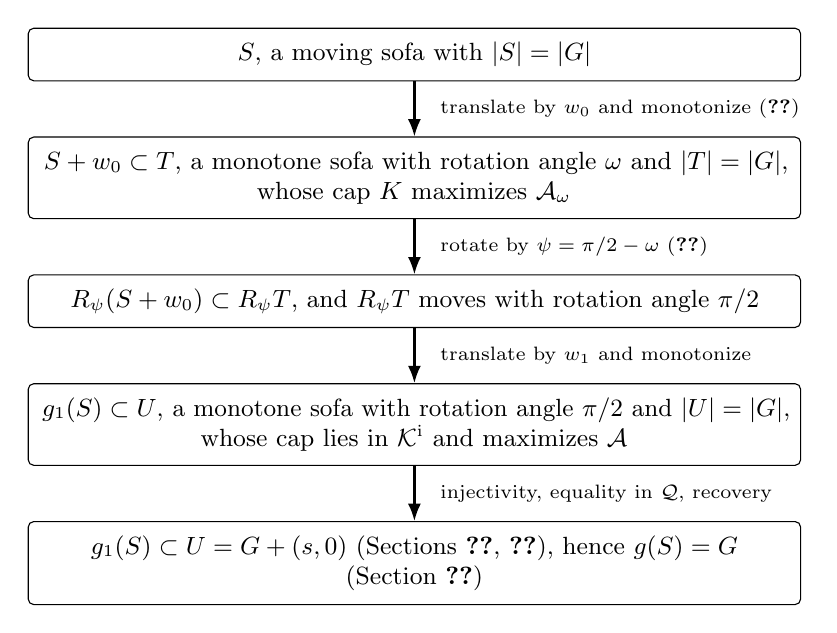
\begin{tikzpicture}[
  node distance=7mm and 0mm,
  box/.style={draw,rounded corners=2pt,inner sep=5pt,align=flush center,text width=0.78\linewidth,font=\small},
  arr/.style={-{Latex[length=2.2mm]},thick},
  lab/.style={font=\scriptsize,anchor=west,align=left}]
  \node[box] (S) {$S$, a moving sofa with $\abs S=\abs\Gs$};
  \node[box,below=of S] (T) {$S+w_0\subset T$, a monotone sofa with rotation angle $\omega$ and $\abs T=\abs\Gs$, whose cap $K$ maximizes $\cA_\omega$};
  \node[box,below=of T] (R) {$R_\psi(S+w_0)\subset R_\psi T$, and $R_\psi T$ moves with rotation angle $\pi/2$};
  \node[box,below=of R] (U) {$g_1(S)\subset U$, a monotone sofa with rotation angle $\pi/2$ and $\abs U=\abs\Gs$, whose cap lies in $\Ki$ and maximizes $\cA$};
  \node[box,below=of U] (G) {$g_1(S)\subset U=\Gs+(s,0)$ (Sections~\ref{sec:injectivity}, \ref{sec:equality}), hence $g(S)=\Gs$ (Section~\ref{sec:recovery})};
  \draw[arr] (S) -- node[lab,xshift=2mm]{translate by $w_0$ and monotonize (\cref{prop:reduction})} (T);
  \draw[arr] (T) -- node[lab,xshift=2mm]{rotate by $\psi=\pi/2-\omega$ (\cref{sec:right-angle})} (R);
  \draw[arr] (R) -- node[lab,xshift=2mm]{translate by $w_1$ and monotonize} (U);
  \draw[arr] (U) -- node[lab,xshift=2mm]{injectivity, equality in $\cQ$, recovery} (G);
\end{tikzpicture}
\caption{The containment chain of the proof. Every set contains the image of $S$
under the maps so far, and all the sets have area $\abs\Gs$; the first three
arrows are a translation followed by a monotonization, a rotation, and a
translation followed by a monotonization. Here $g_1(p)=R_\psi(p+w_0)+w_1$ and
$g(p)=g_1(p)-(s,0)$.}
\label{fig:chain}
\end{figure}

\section{Approximating a maximizing cap by polygon caps}\label{sec:selection}

In this section and in \cref{sec:variations} we fix $\omega\in(0,\pi/2]$ and a maximizing cap
$K_*\in\Kc_\omega$ with $\cA_\omega(K_*)>0$, and write $h_*=h_{K_*}$. \Cref{sec:right-angle} uses them for the cap of \cref{prop:reduction},
which qualifies since $\abs\Gs>11/5$. \Cref{sec:injectivity} uses them again, with $\omega=\pi/2$, for the cap of the monotone sofa $U$ of \cref{prop:U}, which
qualifies since its sofa area is $\abs\Gs>0$.

Baek approximates a cap by maximum polygon caps and proves that these are balanced; he then takes the
limit of a particular sequence of maximum polygon caps. This procedure need not reach a given maximizing
cap: if $F_n\downarrow F$ uniformly on $[0,1]$, a maximizer of $F$ need not be a limit of
maximizers of the $F_n$ (take $F_n(x)=x/n$ and $F=0$, whose maximizers are all of $[0,1]$ while those of
$F_n$ are $\{1\}$). We therefore subtract a penalty that vanishes at the chosen maximizer, as in the
example $F_n(x)-(x-x_*)^2$, whose maximizers converge to $x_*$. The penalty is a weighted sum of squared
differences of support values at dyadic normals. \cref{sec:variations} bounds the resulting departure from balance.

\subsection{Dyadic angles and the penalty}

For $k\ge0$ let $\Theta_k=\{i\omega/2^{k+1}:0<i<2^{k+1}\}$, an angle set with $2^{k+1}$ intervals and
$\abs{\Theta_k}=2^{k+1}-1$. Then $\Theta_k\subset\Theta_{k+1}$, $\omega/2\in\Theta_k$, and $\bigcup_k\Theta_k$
is dense in $[0,\omega]$. Write $\Kc_k=\Kc_{\Theta_k}$ for the polygon caps with angle set $\Theta_k$ and
$\Theta_k^\diamond$ for the defining normals.

For $m\ge0$ let $\nu_m=2^{-m-1}/\bigl(2(2^{m+1}-1)\bigr)$. For a convex body $K$ and $k\ge0$ let
\[
  \Pi_k(K)=\sum_{m=0}^k\nu_m\sum_{t\in\Theta_m}\Bigl[\bigl(h_K(t)-h_*(t)\bigr)^2+\bigl(h_K(t+\tfrac\pi2)-h_*(t+\tfrac\pi2)\bigr)^2\Bigr].
\]
The terms are the \emph{samples}; an angle of level $m$ also lies in every later level, so it carries one
sample from each level between its first and $k$. For $s\in\R$ let $\nu_k(s)\ge0$ be the total weight of the
samples taken at the normal $s$, so that $\nu_k(s)=0$ unless $s\in\Theta_k\cup(\Theta_k+\pi/2)$. The samples of
level $m$ have total weight $2\abs{\Theta_m}\nu_m=2^{-m-1}$, hence
\begin{equation}\label{eq:weights}
  \sum_s\nu_k(s)=\sum_{m=0}^k2^{-m-1}=1-2^{-k-1}<1 .
\end{equation}
Two elementary facts about $\Pi_k$ will be used. First, \emph{persistence}: if $m\le k$ and $t\in\Theta_m$, then
\begin{equation}\label{eq:persistence}
  \nu_m\bigl(h_K(s)-h_*(s)\bigr)^2\le\Pi_k(K)\qquad(s=t\text{ and }s=t+\pi/2),
\end{equation}
because every term of $\Pi_k$ is nonnegative. Second, if $\abs{h_K(s)-h_*(s)}\le\eta$ at every sample,
and $K'$ is a convex body, then
\begin{equation}\label{eq:penalty-change}
  \bigl\lvert\Pi_k(K')-\Pi_k(K)\bigr\rvert\le\sum_s\nu_k(s)\,\bigl(2\eta r_s+r_s^2\bigr),\qquad r_s=\abs{h_{K'}(s)-h_K(s)},
\end{equation}
where the sum is over the sampled normals $s$; this is the identity
$(b-c)^2-(a-c)^2=2(a-c)(b-a)+(b-a)^2$ applied to each term. In particular, if $K'$ has the same
support values as $K$ at every sampled normal other than one normal $s_0$, where they differ by at most $r$, then
$\abs{\Pi_k(K')-\Pi_k(K)}\le\nu_k(s_0)(2\eta r+r^2)$.

\begin{definition}[penalized maximizer]\label{def:penmax}
A polygon cap $K\in\Kc_k$ is a \emph{penalized maximizer at stage $k$} if
$\cA_{\Theta_k}(C)-\Pi_k(C)\le\cA_{\Theta_k}(K)-\Pi_k(K)$ for every $C\in\Kc_k$.
\end{definition}

\begin{lemma}[recovery polygon]\label{lem:recovery}
$K^{\mathrm r}_k=\cC_{\Theta_k}(K_*)\in\Kc_k$ has $\Pi_k(K^{\mathrm r}_k)=0$ and $\cA_{\Theta_k}(K^{\mathrm r}_k)\ge\cA_\omega(K_*)$.
\end{lemma}

\begin{proof}
By \cref{fact:polygon}, $K^{\mathrm r}_k$ is a polygon cap with the support values of $K_*$ on $\Theta_k^\diamond$, which
contain all the sampled normals; so $\Pi_k(K^{\mathrm r}_k)=0$. Also
$\cA_{\Theta_k}(K^{\mathrm r}_k)=\cA_{\Theta_k}(K_*)\ge\cA_\omega(K_*)$.
\end{proof}

\begin{lemma}[two samples bound a cap]\label{lem:box}
Let $K\in\Kc_k$, $t\in\Theta_k$, and suppose that $q\,(h_K(s)-h_*(s))^2\le c$ for $s=t$ and $s=t+\pi/2$,
with $q>0$, $c\ge0$. Then $K\subset[-R,R]\times[0,1]$ with
$R=H/\sin t+H/\cos t$, $H=\abs{h_*(t)}+\abs{h_*(t+\pi/2)}+c/q+1$.
\end{lemma}

\begin{proof}
From $x^2\le c/q$ follows $\abs x\le c/q+1$, so $h_K(t)\le H$ and $h_K(t+\pi/2)\le H$. A point $(x,y)\in K$ has
$0\le y\le1$, since $K\subset P_\omega$. As $t\in(0,\pi/2)$, $x\cos t+y\sin t\le H$ gives $x\le H/\cos t$,
and $-x\sin t+y\cos t\le H$ gives $-x\le H/\sin t$.
\end{proof}

\begin{lemma}[the niche lies in a box]\label{lem:nichebox}
If $K\in\Kc_\omega$ and $K\subset[-R,R]\times[0,1]$, then $\cN(K)\subset[-R,R]\times[0,R]$; the same holds
for $\cN_\Theta(K)\subset\cN(K)$.
\end{lemma}

\begin{proof}
Let $p\in\cN(K)$, so $p_y\ge0$ and $p\in Q^-_K(t)$ for some $t\in(0,\omega)$. As $K\subset[-R,R]\times[0,1]$,
$h_K(t)\le R\cos t+\sin t\le R\cos t+1$ and $h_K(t+\pi/2)\le R\sin t+\cos t\le R\sin t+1$. So
$\ip p{u_t}<R\cos t$ and $\ip p{v_t}<R\sin t$. Since $p_y\ge0$ and $\ip p{u_t}=p_x\cos t+p_y\sin t$, we get
$p_x<R$; likewise $\ip p{v_t}=-p_x\sin t+p_y\cos t$ gives $p_x>-R$. Finally
$p_y=\sin t\ip p{u_t}+\cos t\ip p{v_t}<2R\sin t\cos t\le R$.
\end{proof}

The proof of the next proposition uses the bounded width of polygon caps of positive area
(\cref{fact:width}), whose proof needs the fan in the definition of $\cN_\Theta$ (E6).

\begin{proposition}[penalized maximizers exist]\label{prop:penmax}
For every $k\ge0$ there is a penalized maximizer $K^{(k)}$ at stage $k$, and
\[
  \cA_{\Theta_k}(K^{(k)})-\Pi_k(K^{(k)})\ge\cA_\omega(K_*).
\]
There is $R_0<\infty$ such that $K^{(k)}\subset[-R_0,R_0]\times[0,1]$ for every $k$.
\end{proposition}

\begin{proof}
Let $\Psi_k=\cA_{\Theta_k}-\Pi_k$ on $\Kc_k$, and $\bar t=\omega/2\in\Theta_k$; the constant $c=c_{\omega,\bar t}$ of \cref{fact:width} does not
depend on $k$. Let $C\in\Kc_k$ with $\Psi_k(C)>0$. Then $\cA_{\Theta_k}(C)>0$, so $C$ has width at most $c$ and, as it
lies in a strip of height one, $\abs C\le c$; hence
$\Pi_k(C)<\cA_{\Theta_k}(C)\le\abs C\le c$ and $\Psi_k(C)\le c$. The samples of level $0$ lie at $\bar t$ and $\bar t+\pi/2$ and have
weight $\nu_0=1/4$ at every stage, so by \eqref{eq:persistence}
$\nu_0(h_C(s)-h_*(s))^2\le\Pi_k(C)\le c$ for $s=\bar t,\bar t+\pi/2$, and \cref{lem:box} puts $C$ in
$[-R_0,R_0]\times[0,1]$ with $R_0$ independent of $k$ and $C$.

By \cref{lem:recovery}, $M_k=\sup\Psi_k\ge\Psi_k(K^{\mathrm r}_k)\ge\cA_\omega(K_*)>0$, and $M_k\le c$. Take $C_j\in\Kc_k$ with
$\Psi_k(C_j)>0$ and $\Psi_k(C_j)\to M_k$. They lie in the box, so by Blaschke's theorem a subsequence converges
in $\dH$ to a convex body $K_\infty$. We show that $K_\infty$ is a penalized maximizer. First, $K_\infty$ is a polygon cap
with angle set $\Theta_k$. Its support values at $\omega,\pi/2,\omega+\pi,3\pi/2$ are $1,1,0,0$ as those of
the $C_j$, and $\abs{K_\infty}=\lim\abs{C_j}\ge\lim\Psi_k(C_j)=M_k>0$ since $\abs{C_j}\ge\cA_{\Theta_k}(C_j)\ge\Psi_k(C_j)$, so $K_\infty$ has an
interior point $q$. Let $p$ lie in $K'_\infty=\bigcap_sH_{K_\infty}(s)$, the intersection over
$s\in\Theta_k^\diamond\cup\{\omega+\pi,3\pi/2\}$. For $0\le\lambda<1$ the point $q+\lambda(p-q)$ satisfies
$\ip{\cdot}{u_s}<h_{K_\infty}(s)$ for all these $s$, hence $\ip\cdot{u_s}\le h_{C_j}(s)$ for large $j$, so it lies in
$C_j$ (a polygon cap is the intersection of its supporting half-planes at these normals), hence in $K_\infty$. As
$K_\infty$ is closed, $p\in K_\infty$; so $K_\infty=K'_\infty$ is a polygon cap. Second, $\Psi_k(K_\infty)\ge\limsup\Psi_k(C_j)$. The
penalty is continuous in the support values. The area is continuous. Each point of $\cN_{\Theta_k}(K_\infty)$
lies in $\cN_{\Theta_k}(C_j)$ for all large $j$: the two strict inequalities defining $Q^-_{K_\infty}(t)$ hold at the point,
and persist when the support values converge. These niches lie in $[-R_0,R_0]\times[0,R_0]$ by \cref{lem:nichebox} (so their areas are finite), and Fatou's lemma gives
$\abs{\cN_{\Theta_k}(K_\infty)}\le\liminf\abs{\cN_{\Theta_k}(C_j)}$. Hence $\cA_{\Theta_k}(K_\infty)\ge\limsup\cA_{\Theta_k}(C_j)$ and
$\Psi_k(K_\infty)\ge M_k$. Put $K^{(k)}=K_\infty$.
\end{proof}

\subsection{Convergence to the given cap}

\begin{lemma}[limits of polygon caps with nested angle sets]\label{lem:limsup}
Let $k_1<k_2<\cdots$ and let $C_j\in\Kc_{k_j}$ lie in a common box $[-R,R]\times[0,1]$ and converge in $\dH$ to $K_\infty\in\Kc_\omega$.
Then $\limsup_j\cA_{\Theta_{k_j}}(C_j)\le\cA_\omega(K_\infty)$.
\end{lemma}

\begin{proof}
By continuity of the area, $\abs{C_j}\to\abs{K_\infty}$. Let $p\in\cN(K_\infty)$: $p\in F_\omega\cap Q_{K_\infty}^-(t)$ for some $t\in(0,\omega)$. The two
strict inequalities that define $Q^-_{K_\infty}(t)$ hold at $p$ with a margin $\delta>0$ at some dyadic angle $t'$ near $t$,
since $h_{K_\infty}$ is continuous. For large $j$, $t'\in\Theta_{k_j}$ and $\sup\abs{h_{C_j}-h_{K_\infty}}<\delta/2$, so
$p\in F_\omega\cap Q^-_{C_j}(t')\subset\cN_{\Theta_{k_j}}(C_j)$. The sets $\cN_{\Theta_{k_j}}(C_j)$ lie in $[-R,R]\times[0,R]$ by \cref{lem:nichebox} (so their areas are finite), and Fatou's lemma gives
$\abs{\cN(K_\infty)}\le\liminf\abs{\cN_{\Theta_{k_j}}(C_j)}$. Subtract.
\end{proof}

\begin{lemma}[dyadic supports determine a cap]\label{lem:dyadic}
If $K,K'\in\Kc_\omega$ and $h_K(s)=h_{K'}(s)$ for all $s\in\bigcup_m\bigl(\Theta_m\cup(\Theta_m+\pi/2)\bigr)$, then $K=K'$.
\end{lemma}

\begin{proof}
By continuity and density, $h_K=h_{K'}$ on $J_\omega$, and $h_K=h_{K'}=0$ at $\omega+\pi$ and $3\pi/2$. A cap is the
intersection of its supporting half-planes at the normals of $J_\omega\cup\{\omega+\pi,3\pi/2\}$.
\end{proof}

\begin{proposition}[selection]\label{prop:selection}
There are $k_1<k_2<\cdots$ and penalized maximizers $K_j$ at stage $k_j$, all in $[-R_0,R_0]\times[0,1]$, such that
$K_j\to K_*$ in $\dH$.
\end{proposition}

\begin{proof}
Take the penalized maximizers $K^{(k)}$ of \cref{prop:penmax}. By Blaschke's theorem there are $k_1<k_2<\cdots$
with $K_j=K^{(k_j)}\to K_\infty$ for a convex body $K_\infty$.

\emph{$K_\infty$ is a cap with rotation angle $\omega$.} The support values at $\omega,\pi/2,\omega+\pi,3\pi/2$ pass to
the limit. Let $(a,b)$ be a gap of $J_\omega\cup\{\omega+\pi,3\pi/2\}$ in the circle; it has length at most
$\pi/2$. A polygon cap $K_j$ has no normal angle strictly between $a$ and $b$, so the supporting lines
$l_{K_j}(a)$ and $l_{K_j}(b)$ meet at a vertex $q$ of $K_j$ and $h_{K_j}(r)=\ip q{u_r}$ for $a\le r\le b$; with
$\sin(b-a)u_r=\sin(b-r)u_a+\sin(r-a)u_b$ this gives
$\sin(b-a)h_{K_j}(r)=\sin(b-r)h_{K_j}(a)+\sin(r-a)h_{K_j}(b)$. The identity passes to $h_{K_\infty}$, and its
coefficients are nonnegative, so $H_{K_\infty}(a)\cap H_{K_\infty}(b)\subset H_{K_\infty}(r)$. Hence $K_\infty=\bigcap_rH_{K_\infty}(r)$ is the
intersection of the $H_{K_\infty}(r)$ with $r\in J_\omega\cup\{\omega+\pi,3\pi/2\}$.

\emph{The penalties tend to $0$.} By \cref{prop:penmax}, $0\le\Pi_{k_j}(K_j)\le\cA_{\Theta_{k_j}}(K_j)-\cA_\omega(K_*)$. By
\cref{lem:limsup} and the maximality of $K_*$, $\limsup_j\cA_{\Theta_{k_j}}(K_j)\le\cA_\omega(K_\infty)\le\cA_\omega(K_*)$.
So $\Pi_{k_j}(K_j)\to0$.

\emph{$K_\infty=K_*$.} Let $t\in\Theta_m$. For $k_j\ge m$, \eqref{eq:persistence} gives
$\nu_m(h_{K_j}(s)-h_*(s))^2\le\Pi_{k_j}(K_j)\to0$ for $s=t,t+\pi/2$, while $h_{K_j}(s)\to h_{K_\infty}(s)$. So
$h_{K_\infty}=h_*$ at all dyadic normals, and $K_\infty=K_*$ by \cref{lem:dyadic}. The box is \cref{prop:penmax}.
\end{proof}

Put $\eta_j=\dH(K_j,K_*)\to0$. At every sampled normal, $\abs{h_{K_j}(s)-h_*(s)}\le\eta_j$.

\section{Penalized maximizers are almost balanced}\label{sec:variations}

A maximum polygon cap is balanced \baek{Thm.~3.4.9}: $\sigma_K(t)=\tau_K(t)$ for
every $t\in\Theta^\diamond$, since otherwise pushing one side would increase
$\cA_\Theta$. A penalized maximizer need not be balanced, but pushing a side
changes the penalty by a controlled amount, and the argument gives a one-sided
bound on the \emph{defect}
\[
  \zeta_K(t)=\sigma_K(t)-\tau_K(t).
\]
In this section we fix $k\ge0$, $\Theta=\Theta_k$, a penalized maximizer
$K\in\Kc_k$ at stage $k$, and $\eta\ge0$ with $\abs{h_K(s)-h_*(s)}\le\eta$ at
every sampled normal $s$. Let
\[
  \bar\nu=\sum_s\nu_k(s)
\]
be the total weight; $\bar\nu\le1$ by \eqref{eq:weights}.

\begin{figure}[ht]
\centering
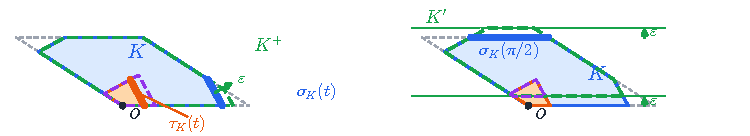
\includegraphics[width=\linewidth]{figures/fig-moves}
\caption{Pushing one side of a polygon cap $K$ with angle set $\{\omega/2\}$,
$\omega=1$; the grey dashed parallelogram is $P_\omega$, and the niche of $K$ is
orange. Left: raising the height at the floating normal $t=\omega/2$ by $\eps$
gives the cap $K^+$ (green, dashed) and its niche (purple, dashed); the cap
gains a strip of area $\sigma_K(t)\eps+O(\eps^2)$ along its edge with normal
$t$, and the niche a strip of area $\tau_K(t)\eps+O(\eps^2)$ along the side on
the inner wall $b_K(t)$. Right: raising the pinned height at $\pi/2$ by $\eps$
moves both lines of the horizontal strip up by $\eps$ (green, dotted) and gives
$K'$ (green, dashed), with its niche (purple, dashed); the cap gains a strip
along its top edge, of length $\sigma_K(\pi/2)$, and loses one along its bottom
edge, and $K'$ is a translate of a polygon cap.}
\label{fig:moves}
\end{figure}

\subsection{Floating normals}

\begin{lemma}[raising a floating height]\label{lem:floating}
Let $K\in\Kc_\Theta$, $t\in\Theta^\diamond\setminus\{\omega,\pi/2\}$,
$\eps\ge0$, and $K^+=\cC_\Theta(h_K^{t,\eps})$. Then $K^+\in\Kc_\Theta$,
$K\subset K^+$, and
\[
  h_{K^+}(s)=h_K(s)\quad\text{for }s\in\Theta^\diamond\setminus\{t\},\qquad
  h_K(t)\le h_{K^+}(t)\le h_K(t)+\eps.
\]
\end{lemma}

\begin{proof}
Since $h_K(\omega)=h_K(\pi/2)=1$, $P_{h^{t,\eps}_K}=P_\omega$, so
\[
  K^+=P_\omega\cap\bigcap_sH_-\bigl(s,h^{t,\eps}_K(s)\bigr),
\]
the intersection over the floating normals $s$. As $h_K\le h^{t,\eps}_K$,
\[
  K=\cC_\Theta(h_K)\subset K^+\subset P_\omega.
\]
So $K^+$ is a convex body (it is bounded, since the half-planes with normals
$t'$ and $t'+\pi/2$, $t'\in\Theta$, bound it also when $\omega=\pi/2$), it has
the support values $1,1,0,0$ of $P_\omega$ at $\omega,\pi/2,\omega+\pi,3\pi/2$,
and it is an intersection of half-planes with the normal angles of a polygon
cap. So $K^+\in\Kc_\Theta$. Next, $h_{K^+}\ge h_K$ since $K\subset K^+$, and
$h_{K^+}(s)\le h_K^{t,\eps}(s)$ since $K^+\subset H_-(s,h^{t,\eps}_K(s))$.
\end{proof}

\begin{proposition}[floating defects]\label{prop:floating}
For every floating normal $t\in\Theta^\diamond\setminus\{\omega,\pi/2\}$,
\[
  \sigma_K(t)-\tau_K(t)\le2\eta\,\nu_k(t).
\]
\end{proposition}

\begin{proof}
Let $K^+_\eps=\cC_\Theta(h^{t,\eps}_K)$. By \cref{lem:floating}, $K^+_\eps$ is a
polygon cap that has the support values of $K$ on
$\Theta^\diamond\setminus\{t\}$, and differs from $K$ at $t$ by at most $\eps$;
so by \eqref{eq:penalty-change-one},
\[
  \Pi_k(K^+_\eps)-\Pi_k(K)\le\nu_k(t)(2\eta\eps+\eps^2).
\]
Penalized maximality gives
$\cA_\Theta(K^+_\eps)-\cA_\Theta(K)\le\Pi_k(K^+_\eps)-\Pi_k(K)$. By
\cref{fact:push}\ref{fact:push:area} (with $C=K^+_\eps$, $v=0$) and
\ref{fact:push:derivative}, for small $\eps$
\[
  \cA_\Theta(K^+_\eps)\ge\cA_\Theta(h_K^{t,\eps})\ge\cA_\Theta(K)+(\sigma_K(t)
    -\tau_K(t))\eps-M\eps^2 .
\]
Hence
\[
  (\sigma_K(t)-\tau_K(t))\eps-M\eps^2\le\nu_k(t)(2\eta\eps+\eps^2).
\]
Divide by $\eps$ and let $\eps\to0$.
\end{proof}

\subsection{Pinned normals}

In this subsection $\omega<\pi/2$, so that the two pinned normals $\omega$ and
$\pi/2$ are distinct and every cap contains $O$ and $o_\omega$
(\cref{lem:contains}); in particular $h_K\ge0$. Moving a pinned normal moves
both lines of a strip, and the result is in general only a translate of a
polygon cap.

\begin{lemma}[the pinned sandwich]\label{lem:sandwich}
Let $K\in\Kc_\Theta$, $t\in\{\omega,\pi/2\}$, $\eps\in[0,1]$, and
$K'=\cC_\Theta(h_K^{t,\eps})$. Then
\[
  (1-\eps)K+\eps\,o_\omega\subset K'\subset(1+\eps)K .
\]
If $R\ge0$ and $\abs{h_K(s)}\le R$ for all $s$, then
\[
  \abs{h_{K'}(s)-h_K(s)}\le2R\eps\quad\text{for every }s.
\]
\end{lemma}

\begin{proof}
Let $t'$ be the other pinned normal. Then
\begin{multline*}
  K'=\{p:\ \eps\le\ip p{u_t}\le1+\eps,\ 0\le\ip p{u_{t'}}\le1,\\
    \ip p{u_s}\le h_K(s)\text{ for floating }s\}.
\end{multline*}
Let $p\in K$ and $q=(1-\eps)p+\eps o_\omega\in K$. Then $q$ satisfies every
inequality of $K'$ except possibly the one for $t$, and
\[
  \ip q{u_t}=(1-\eps)\ip p{u_t}+\eps\in[\eps,1],
\]
because $\ip{o_\omega}{u_t}=1$ and $0\le\ip p{u_t}\le1$. So $q\in K'$.
Conversely, let $p\in K'$. For floating $s$,
\[
  \ip{p/(1+\eps)}{u_s}\le h_K(s)/(1+\eps)\le h_K(s),
\]
as $h_K(s)\ge0$; $\ip p{u_t}/(1+\eps)\in[0,1]$ and $\ip
p{u_{t'}}/(1+\eps)\in[0,1]$. So ${p/(1+\eps)\in K}$. Taking support functions,
\[
  (1-\eps)h_K(s)+\eps\ip{o_\omega}{u_s}\le h_{K'}(s)\le(1+\eps)h_K(s).
\]
As $o_\omega\in K$, $-\ip{o_\omega}{u_s}=\ip{o_\omega}{u_{s+\pi}}\le
h_K(s+\pi)\le R$; with $\abs{h_K(s)}\le R$ this gives $-2R\eps\le
h_{K'}(s)-h_K(s)\le R\eps$.
\end{proof}

\begin{lemma}[moving back to standard position]\label{lem:back}
Let $K\in\Kc_\Theta$, $t\in\{\omega,\pi/2\}$, $\eps\ge0$, and suppose that
$K'=\cC_\Theta(h_K^{t,\eps})$ is a translate $C+v$ of a polygon cap
$C\in\Kc_\Theta$, $v\in\R^2$. Then
\[
  \abs{\ip v{u_s}}\le(2/\cos\omega+1)\eps\quad\text{for all }s.
\]
If moreover $\eps\le1$, $R\ge0$ and $\abs{h_K(s)}\le R$ for all $s$, then
\[
  \abs{h_C(s)-h_K(s)}\le \gamma(R)\,\eps\quad\text{for every }s,\qquad \gamma(R)
    =2R+\frac2{\cos\omega}+1 .
\]
\end{lemma}

\begin{proof}
Let $t'$ be the other pinned normal. For $s\in\{\omega,\pi/2\}$, $K'$ lies in
the strip $a_s\le\ip p{u_s}\le a_s+1$, where $a_t=\eps$ and $a_{t'}=0$. As $C$
is a cap, it has width exactly $1$ in the direction $u_s$ (its support values at
$s$ and $s+\pi$ are $1$ and $0$), and so has $C+v$; hence $\ip v{u_s}=a_s$. With
$s=\pi/2$ and $s=\omega$ this gives
\[
  v_y\in[0,\eps],\qquad v_x\cos\omega+v_y\sin\omega\in[0,\eps],
\]
so $\abs{v_x}\le2\eps/\cos\omega$ and
\[
  \abs{\ip v{u_s}}\le\abs{v_x}+\abs{v_y}\le(2/\cos\omega+1)\eps.
\]
Finally $h_C(s)=h_{K'}(s)-\ip v{u_s}$, and \cref{lem:sandwich} gives
$\abs{h_{K'}(s)-h_K(s)}\le2R\eps$; so
\[
  \abs{h_C(s)-h_K(s)}\le2R\eps+(2/\cos\omega+1)\eps=\gamma(R)\eps.\qedhere
\]
\end{proof}

\begin{proposition}[pinned defects]\label{prop:pinned}
Let $\omega<\pi/2$, $R\ge0$ with $\abs{h_K(s)}\le R$ for all $s$, and
$t\in\{\omega,\pi/2\}$. Then
\[
  \sigma_K(t)-\tau_K(t)\le2\bar\nu\eta\,\gamma(R),\qquad \gamma(R)=2R
    +\frac2{\cos\omega}+1 .
\]
\end{proposition}

\begin{proof}
If $\sigma_K(t)=0$, the left side is $-\tau_K(t)\le0$. Let $\sigma_K(t)>0$. By
\cref{fact:push}\ref{fact:push:translate}, for small $\eps\in(0,1]$ the set
$\cC_\Theta(h_K^{t,\eps})$ is a translate $C_\eps+v_\eps$ of a polygon cap
$C_\eps$. By \cref{lem:back}, $\abs{h_{C_\eps}(s)-h_K(s)}\le \gamma(R)\eps$ at
every $s$, so \eqref{eq:penalty-change} gives
\[
  \Pi_k(C_\eps)-\Pi_k(K)\le\bar\nu(2\eta\gamma(R)\eps+\gamma(R)^2\eps^2).
\]
Penalized maximality compares $K$ with $C_\eps$, and
\cref{fact:push}\ref{fact:push:area}, \ref{fact:push:derivative} give
\[
  \cA_\Theta(C_\eps)\ge\cA_\Theta(h_K^{t,\eps})\ge\cA_\Theta(K)+(\sigma_K(t)
    -\tau_K(t))\eps-M\eps^2 .
\]
So
\[
  (\sigma_K(t)-\tau_K(t))\eps-M\eps^2\le\bar\nu(2\eta\gamma(R)\eps
    +\gamma(R)^2\eps^2);
\]
divide by $\eps$ and let $\eps\to0$.
\end{proof}

\subsection{A two-sided bound}

\begin{corollary}[two-sided defect bound]\label{cor:twosided}
Let $\omega<\pi/2$, and $R\ge0$ with $\abs{h_K(s)}\le R$ for all $s$. For every
$t\in\Theta^\diamond$,
\[
  \abs{\sigma_K(t)-\tau_K(t)}
    \le\frac{2\bar\nu\eta+4\bar\nu\eta\gamma(R)}{\sin t},\qquad \gamma(R)=2R
    +\frac2{\cos\omega}+1 .
\]
\end{corollary}

\begin{proof}
Put $\zeta(s)=\sigma_K(s)-\tau_K(s)$, and
\[
  e(s)=2\eta\nu_k(s)\quad\text{for floating }s,\qquad
  e(s)=2\bar\nu\eta\gamma(R)\quad\text{for the two pinned }s.
\]
By \cref{prop:floating,prop:pinned}, $\zeta\le e$ on $\Theta^\diamond$, and
$e\ge0$ with
\[
  \sum_se(s)\le2\bar\nu\eta+4\bar\nu\eta\gamma(R)=:E.
\]
By \cref{fact:sides}\ref{fact:sides:identity}, the sums
$\sum_s\sigma_K(s)\sin s$ and $\sum_s\tau_K(s)\sin s$ both equal
$A_K^-(0)_x-C_K^+(\omega)_x$, so $\sum_s\sin s\,\zeta(s)=0$; and $0<\sin s\le1$
on $\Theta^\diamond\subset(0,\pi)$. So
\begin{align*}
  \sin t\,\zeta(t)&=-\sum_{s\ne t}\sin s\,\zeta(s)\ge-\sum_{s\ne t}\sin s\,e(s)
    \ge-E,\\
  \sin t\,\zeta(t)&\le\sin t\,e(t)\le E .\qedhere
\end{align*}
\end{proof}

\section{The pinned bounds and the right angle}\label{sec:right-angle}

Baek shows that a balanced maximum sofa $S_\omega$ with $\abs{S_\omega}\ge11/5$ and rotation angle $\omega\in[\omega_0,\pi/2)$
has a rotated copy that turns through the full right angle \baek{Thm.~1.5.2}. The proof uses the balance only
through two inequalities, $w^\circ_K\le\sigma_K(\pi/2)$ and $z^\circ_K\le\sigma_K(\omega)$, which bound the wedge gaps on the two floors $y=0$ and $l(\omega,0)$ by the lengths of the sides of the
cap on the opposite walls $y=1$ and $l(\omega,1)$ \baek{Thm.~4.1.4}. We
prove these inequalities for $K_*$ from the defect bounds of \cref{sec:variations}, and then follow
Baek's proof with them as hypotheses. In \cref{sec:pinned-bounds,sec:triangle} we have $\omega<\pi/2$, and $K_*$ is as in \cref{sec:selection};
\cref{prop:U} also covers $\omega=\pi/2$.

\subsection{The pinned bounds}\label{sec:pinned-bounds}

For a cap $K\in\Kc_\omega$ and $t\in(0,\omega)$ let
\[
  w_K(t)=h_K(0)-\frac{h_K(t)-1}{\cos t},\qquad
  z_K(t)=h_K(\omega+\tfrac\pi2)-\frac{h_K(t+\pi/2)-1}{\cos(\omega-t)},
\]
the \emph{wedge gaps}: with $A=(h_K(0),0)=A_K^-(0)$ and $C=h_K(\omega+\pi/2)v_\omega=C_K^+(\omega)$ the ends of the
upper boundary of $K$ (see \eqref{eq:ends}), $w_K(t)$ is the distance from $A$ to the point
$W_K(t)=((h_K(t)-1)/\cos t,0)$ where the inner wall $b_K(t)$ meets the $x$-axis, and $z_K(t)$ is the
distance from $C$ to the point where $d_K(t)$ meets $l(\omega,0)$ \baek{Def.~2.5.5}. Let
$w^\circ_K=\inf_{t\in(0,\omega)}w_K(t)$ and $z^\circ_K=\inf_{t\in(0,\omega)}z_K(t)$ \baek{Def.~4.1.1}.
As $t\to\omega$, $w_K(t)\to h_K(0)$, so $w^\circ_K\le h_K(0)$; as $t\to0$, $z_K(t)\to h_K(\omega+\pi/2)$, so $z^\circ_K\le h_K(\omega+\pi/2)$.

\begin{lemma}[wedge gaps and the polyline]\label{lem:wedge}
Every polygon cap $K\in\Kc_\Theta$ satisfies $w^\circ_K\le\tau_K(\pi/2)$ and $z^\circ_K\le\tau_K(\omega)$.
\end{lemma}

This is the first half of the proof of \baek{Thm.~4.1.2}.

\begin{proof}
The bottom edge $e_K(3\pi/2)=K\cap\{y=0\}$ is the segment from $O$ to $A=(h_K(0),0)$, so
$\sigma_K(3\pi/2)=h_K(0)$. A point $(x,0)$ of $\cN_\Theta(K)$ lies in $F_\omega$, so $x\ge0$, and in some
$Q^-_K(t)$, $t\in\Theta$, so $x\cos t<h_K(t)-1$, that is $x<h_K(0)-w_K(t)\le h_K(0)-w_K^\circ$. Hence
$\cN_\Theta(K)\cap\{y=0\}\subset[0,h_K(0)-w^\circ_K)\times\{0\}$, and by \cref{fact:sides}\ref{fact:sides:floor}
\begin{align*}
  h_K(0)-\tau_K(\pi/2)&=\sigma_K(3\pi/2)-\tau_K(\pi/2)\\
  &=\Hone\bigl(\cN_\Theta(K)\cap l(\pi/2,0)\bigr)\le h_K(0)-w^\circ_K,
\end{align*}
where we used $w^\circ_K\le h_K(0)$. The second inequality is the same argument on the line $l(\omega,0)$, with
the bottom edge $e_K(\omega+\pi)=[O,C]$ of length $\sigma_K(\omega+\pi)=h_K(\omega+\pi/2)$, the points
$\lambda v_\omega$ of $Q^-_K(t)$, which have $\lambda<h_K(\omega+\pi/2)-z_K(t)$, and
\cref{fact:sides}\ref{fact:sides:floor} with $t=\omega$.
\end{proof}

\begin{lemma}[continuity]\label{lem:cont}
For caps $K,K'\in\Kc_\omega$ with $\dH(K,K')=\eps$, $\abs{w^\circ_K-w^\circ_{K'}}\le(1+\sec\omega)\eps$ and
$\abs{z^\circ_K-z^\circ_{K'}}\le(1+\sec\omega)\eps$.
\end{lemma}

\begin{proof}
For $t\in(0,\omega)$, $\abs{w_K(t)-w_{K'}(t)}\le\eps+\eps\sec t\le(1+\sec\omega)\eps$; similarly for $z$, since
$\cos(\omega-t)\ge\cos\omega$. The infima differ by at most as much. \baek{Lemma~4.1.1}
\end{proof}

Baek obtains \baek{Thm.~4.1.4} from the weak convergence of surface area measures \baek{Thm.~4.1.3} and the Portmanteau theorem. The following elementary
lemma, which uses only support functions, replaces that step.

\begin{lemma}[upper semicontinuity of edge lengths]\label{lem:usc}
If convex bodies $K_j\to K$ in $\dH$, then $\limsup_j\sigma_{K_j}(t)\le\sigma_K(t)$ for every $t$.
\end{lemma}

\begin{proof}
For $0<\delta<\pi$,
\begin{align*}
  h_K(t+\delta)&\ge\ip{v_K^+(t)}{u_{t+\delta}}=h_K(t)\cos\delta+\ip{v_K^+(t)}{v_t}\sin\delta,\\
  h_K(t-\delta)&\ge\ip{v_K^-(t)}{u_{t-\delta}}=h_K(t)\cos\delta-\ip{v_K^-(t)}{v_t}\sin\delta.
\end{align*}
Adding, and using $\sigma_K(t)=\ip{v_K^+(t)-v_K^-(t)}{v_t}$,
\[
  \sigma_K(t)\le\Delta_K(\delta)=\frac{h_K(t+\delta)+h_K(t-\delta)-2h_K(t)\cos\delta}{\sin\delta}.
\]
$\Delta_K(\delta)$ depends continuously on the values of $h_K$, so $\Delta_{K_j}(\delta)\to\Delta_K(\delta)$ and
$\limsup_j\sigma_{K_j}(t)\le\Delta_K(\delta)$ for every $\delta$. By \cref{fact:convex}\ref{fact:convex:vertices},
$\Delta_K(\delta)\to\ip{v_K^+(t)-v_K^-(t)}{v_t}=\sigma_K(t)$ as $\delta\downarrow0$.
\end{proof}

\begin{proposition}[pinned bounds]\label{prop:pinned-bounds}
$w^\circ_{K_*}\le\sigma_{K_*}(\pi/2)$ and $z^\circ_{K_*}\le\sigma_{K_*}(\omega)$.
\end{proposition}

\begin{proof}
Take the selection $K_j\to K_*$ of \cref{prop:selection} in $[-R_0,R_0]\times[0,1]\subset\{\norm p\le R\}$,
$R=R_0+1$, and $\eta_j=\dH(K_j,K_*)\to0$; at every sampled normal $\abs{h_{K_j}-h_*}\le\eta_j$, and the total
weight is $\bar\nu<1$. By \cref{cor:twosided} at $t=\pi/2$, with $e_j=(2+4\gamma_\omega)\eta_j$,
$\abs{\sigma_{K_j}(\pi/2)-\tau_{K_j}(\pi/2)}\le e_j$; so by \cref{lem:wedge}
\[
  w^\circ_{K_j}-e_j\le\tau_{K_j}(\pi/2)-e_j\le\sigma_{K_j}(\pi/2).
\]
By \cref{lem:cont}, $w^\circ_{K_j}\to w^\circ_{K_*}$, and by \cref{lem:usc},
$\limsup_j\sigma_{K_j}(\pi/2)\le\sigma_{K_*}(\pi/2)$. This gives the first inequality. For the second use
$t=\omega$, where \cref{cor:twosided} divides by $\sin\omega>0$.
\end{proof}

\subsection{The triangle in the niche}\label{sec:triangle}

Let $\omega\in[\omega_0,\pi/2)$, so that $\omega>\pi/4$. Put $c=c_\omega=\sec\omega-\tan\omega$, so that
$o_\omega-v_0=c\,u_0$ and $o_\omega-u_\omega=c\,v_\omega$ \baek{Prop.~4.2.1}, and let $\Delta_\omega$ be the
triangle with vertices $O$, $cu_0$, $cv_\omega$, which cuts off the corner $O$ of $P_\omega$. Let
$d_{\min}=5/4$ if $\omega<\tan^{-1}(11/5)$ and $d_{\min}=11/10$ otherwise, and for $d\in[0,\tan\omega]$ let
$R_{\omega,d}=P_\omega\cap H_-(0,d+c)\cap H_-(\omega+\pi/2,d+c)$ be $P_\omega$ without its two acute corners.

\begin{fact}[numerical inequalities at the corner]\label{fact:corner}
Let $\omega\in[\omega_0,\pi/2)$.
\begin{enumerate}[label=(\alph*)]
\item $\abs{R_{\omega,d_{\min}}}<11/5$. \baek{Lemma~4.2.2}
\item If $d\in[d_{\min},\tan\omega]$, $r_y=1-d\cot\omega\ge0$ and $g=\sqrt{1-r_y^2}$, then $d\sin\omega>1$ and $g>2\cos\omega$.
\baek{Lemma~4.2.4, in the range $[\sec^{-1}(2.2),\pi/2)$ of its proof and of its use (E9)}
\end{enumerate}
\end{fact}

\begin{lemma}[the triangle lies in the niche]\label{lem:triangle}
Let $\omega\in[\omega_0,\pi/2)$ and $K\in\Kc_\omega$ with $\cA_\omega(K)\ge11/5$, $w^\circ_K\le\sigma_K(\pi/2)$ and
$z^\circ_K\le\sigma_K(\omega)$. Then for some $t_\sharp\in(0,\omega)$ the three vertices $O$, $cu_0$, $cv_\omega$ of
$\Delta_\omega$ lie in $Q^-_K(t_\sharp)$.
\end{lemma}

This is \baek{Thm.~4.2.5} for a cap that satisfies the pinned bounds, in place of a balanced maximum cap; the
proof there uses balance only through them.

\begin{proof}
\emph{Step 1: a long cap.} Since $\abs K\ge\cA_\omega(K)\ge11/5>\abs{R_{\omega,d_{\min}}}$ and $K\subset P_\omega$,
$K$ is not contained in $R_{\omega,d_{\min}}$, so $h_K(0)\ge d_{\min}+c$ or $h_K(\omega+\pi/2)\ge d_{\min}+c$.
We may assume the first. Otherwise replace $K$ by its mirror image $K^{\mir}$: it is a cap with the same sofa
area, and $h_{K^{\mir}}(0)=h_K(\omega+\pi/2)$, $w^\circ_{K^{\mir}}=z^\circ_K$, $\sigma_{K^{\mir}}(\pi/2)=\sigma_K(\omega)$,
so it satisfies the hypotheses; and since $M_\omega$ fixes $O$, exchanges $cu_0$ and $cv_\omega$ and maps
$Q^-_{K^{\mir}}(t)$ to $Q^-_K(\omega-t)$ \baek{Prop.~2.5.4}, the conclusion for $K^{\mir}$ at $t_\sharp$ is the conclusion
for $K$ at $\omega-t_\sharp$. Put $d=h_K(0)-c\ge d_{\min}$ and $q_0=(h_K(0),0)=A^-_K(0)\in K$. Since $K\subset P_\omega$,
$h_K(0)\le\sec\omega$, so $d\le\tan\omega$, and $q_0=(o_\omega-v_0)+d\,u_0$.

\emph{Step 2: the bottom side.} The lines $l_K(0)$ and $l_K(\omega)=l(\omega,1)$ meet at $r=(h_K(0),r_y)$ with
$r_y=1-d\cot\omega\ge0$ (as $q_0\in P_\omega$). Let $g=\sqrt{1-r_y^2}$ and $s=q_0-g\,u_0$: the triangle
$s,q_0,r$ has a right angle at $q_0$, and $\norm{r-s}=1$. For $t\in(0,\omega)$, $u_t$ is a nonnegative
combination of $u_0$ and $u_\omega$, and $K\subset H_K(0)\cap H_K(\omega)$, so $h_K(t)\le\ip r{u_t}$, and
\[
  h_K(t)-1\le\ip r{u_t}-\ip{r-s}{u_t}=\ip s{u_t}.
\]
So $s$ lies on or to the right of $W_K(t)$, that is $w_K(t)\ge g$. Hence $g\le w^\circ_K$.

\emph{Step 3: the top side.} By hypothesis, $g\le w^\circ_K\le\sigma_K(\pi/2)$. The point $o_\omega$ lies in $K$,
and it is the right end of the top edge $e_K(\pi/2)=K\cap\{y=1\}$, because $K\subset P_\omega$. So
$q_1=o_\omega-g\,u_0$ lies on $e_K(\pi/2)$, and $q_1\in K$.

\emph{Step 4: the hallway of angle $t_\sharp=\pi/2-\omega$.} Note $t_\sharp\in(0,\pi/4)\subset(0,\omega)$. Let $X=\{q_0,q_1\}\subset K$;
then $h_X\le h_K$, so $Q^-_X(t_\sharp)\subset Q^-_K(t_\sharp)$. We have $q_1-q_0=v_0-(d+g)u_0=-\alpha u_{t_\sharp}+\beta v_{t_\sharp}$ with
$\alpha=(d+g)\cos t_\sharp-\sin t_\sharp\ge0$ and $\beta=\cos t_\sharp+(d+g)\sin t_\sharp\ge0$, since $d+g\ge1>\tan t_\sharp$. So
$q_0$ maximizes $\ip\cdot{u_{t_\sharp}}$ and $q_1$ maximizes $\ip\cdot{v_{t_\sharp}}$ on $X$, and
\begin{align*}
  Q^-_X(t_\sharp)&=\{p:\ \ip p{u_{t_\sharp}}<m_1,\ \ip p{v_{t_\sharp}}<m_2\},\\
  m_1&=\ip{q_0}{u_{t_\sharp}}-1,\quad m_2=\ip{q_1}{v_{t_\sharp}}-1 .
\end{align*}

\emph{Step 5: the vertices.} By \cref{fact:corner}(b), $d\sin\omega>1$ and $g>2\cos\omega$. Now
$\ip{q_0-cu_0}{u_{t_\sharp}}=d\sin\omega>1$, so $m_1>c\cos t_\sharp>0$; and
$\ip{q_1-cv_\omega}{v_{t_\sharp}}=\ip{u_\omega-gu_0}{v_{t_\sharp}}=-\cos2\omega+g\cos\omega>1$ (this is
$g>2\cos\omega$, as $1+\cos2\omega=2\cos^2\omega$), so $m_2>c\cos(\omega-t_\sharp)>0$. Then $O$ satisfies both
inequalities. For $cu_0$: $\ip{cu_0}{u_{t_\sharp}}=c\cos t_\sharp<m_1$ and $\ip{cu_0}{v_{t_\sharp}}=-c\sin t_\sharp<0<m_2$. For $cv_\omega$:
$\ip{cv_\omega}{u_{t_\sharp}}=-c\sin(\omega-t_\sharp)<0<m_1$ and $\ip{cv_\omega}{v_{t_\sharp}}=c\cos(\omega-t_\sharp)<m_2$. So the
three points lie in $Q^-_X(t_\sharp)\subset Q^-_K(t_\sharp)$.
\end{proof}

\subsection{A rotated copy turns through the right angle}

\begin{lemma}[the width of the sofa]\label{lem:width}
Let $\omega\in(0,\pi/2)$ and $K\in\Kc_\omega$, and suppose that $O,cu_0,cv_\omega\in Q^-_K(t_\sharp)$ for some
$t_\sharp\in(0,\omega)$. Then
\begin{enumerate}[label=(\alph*)]
\item every point $\lambda u_0+\mu v_\omega$ with $\lambda,\mu\ge0$ and $\lambda+\mu<c$ lies in $\cN(K)$;
\item $\ip{p-q}{u_t}\le1$ for all $p\in K$, $q\in K\setminus\cN(K)$ and $t\in[\omega,\pi/2]$.
\end{enumerate}
\end{lemma}

\begin{proof}
(a) Such a point is a convex combination of $O$, $cu_0$ and $cv_\omega$ with the weights $1-(\lambda+\mu)/c>0$, $\lambda/c$, $\mu/c$.
The open convex set $Q^-_K(t_\sharp)$ contains all three vertices, hence the point, and the point lies in $F_\omega$
since $\ip{u_0}{u_\omega},\ip{v_\omega}{u_\omega},\ip{u_0}{u_{\pi/2}},\ip{v_\omega}{u_{\pi/2}}\ge0$.

(b) Write $q=\lambda u_0+\mu v_\omega$. As $q\in P_\omega$, $\lambda=\ip q{u_\omega}/\cos\omega\ge0$ and $\mu=q_y/\cos\omega\ge0$, and
$\lambda+\mu\ge c$ by (a). For $t\in[\omega,\pi/2]$ both $\cos t$ and $\sin(t-\omega)$ are nonnegative, so
$\ip q{u_t}=\lambda\cos t+\mu\sin(t-\omega)\ge c\min(\cos t,\sin(t-\omega))$, while $\ip p{u_t}\le\ip{o_\omega}{u_t}=c\cos t+\sin t$
as $o_\omega$ is the vertex of $P_\omega$ farthest in these directions. If $\cos t\le\sin(t-\omega)$, then
$\ip{p-q}{u_t}\le\sin t\le1$. Otherwise, using $c(1+\sin\omega)=\cos\omega$ and $c\cos\omega=1-\sin\omega$,
\[
  \ip{p-q}{u_t}\le c\cos t+\sin t-c\sin(t-\omega)=\cos(t-\omega)\le1 .\qedhere
\]
\end{proof}

\begin{lemma}[turning inside the horizontal side]\label{lem:turn}
Let $S$ be a moving sofa with rotation angle $\omega\in(0,\pi/2)$ such that $\ip{p-q}{u_t}\le1$ for all $p,q\in S$ and
$t\in[\omega,\pi/2]$. Then $R_\psi S$, $\psi=\pi/2-\omega$, is a moving sofa with rotation angle $\pi/2$.
\end{lemma}

\begin{proof}
Let $(\theta,\mathbf c)$ be a movement of $S$ with rotation angle $\omega$. For $\rho\in[0,\psi]$ the height of $R_\rho S$,
that is its width in the direction $u_{\pi/2}$, is the width of $S$ in the direction $u_{\pi/2-\rho}$ with
$\pi/2-\rho\in[\omega,\pi/2]$, so it is at most $1$. Hence the translations
$b(\rho)=(1-\max_{p\in S}(R_\rho p)_x,\ -\min_{p\in S}(R_\rho p)_y)$, which depend continuously
on $\rho$, put $R_\rho S+b(\rho)$ in $H_L$. The movement of $R_\psi S$ has three phases: turn clockwise by $\psi$
through the positions $R_\rho S+b(\rho)$, $\rho$ from $\psi$ down to $0$; translate along a segment in
$H_L$, which is convex, from $S+b(0)$ to the starting position $S+\mathbf c(0)$ of the movement of $S$; and follow
that movement. The total rotation is $\psi+\omega=\pi/2$, and $R_\psi S$ is closed and connected.
\end{proof}

\begin{figure}[ht]
\centering
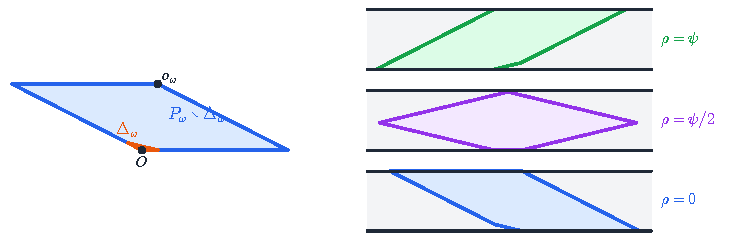
\includegraphics[width=\linewidth]{figures/fig-rotate}
\caption{\cref{lem:width,lem:turn}, for $\omega=1.1$. Left: the parallelogram $P_\omega$ (dashed), its corner triangle $\Delta_\omega$
(orange) and the pentagon $P_\omega\setminus\Delta_\omega$ (blue); the sofa $K\setminus\cN(K)$ lies in the pentagon, up to the far side of $\Delta_\omega$.
Right: the pentagon turned by $\rho=\psi$, $\psi/2$ and $0$, $\psi=\pi/2-\omega$, in a horizontal strip of width one: it fits for
every $\rho\in[0,\psi]$, since its width in the direction $u_t$ is at most $1$ for $t\in[\omega,\pi/2]$.}
\label{fig:rotate}
\end{figure}

\begin{proposition}[a right-angle monotone sofa]\label{prop:U}
Let $\omega\in[\omega_0,\pi/2]$ and let $T$ be a monotone sofa with rotation angle $\omega$, $\abs T=\abs\Gs$, and
cap $K=\cC(T)$, as in \cref{prop:reduction}. Then $R_\psi T$, $\psi=\pi/2-\omega$, is a moving sofa with rotation angle
$\pi/2$. Consequently there are $w_1\in\R^2$ and a monotone sofa $U$ with rotation angle $\pi/2$ such that
\[
  R_\psi T+w_1\subset U,\qquad\abs U=\abs\Gs,
\]
and the cap $\cC(U)\in\Kc_{\pi/2}$ is maximizing, with $\cA(\cC(U))=\abs\Gs$.
\end{proposition}

\begin{proof}
If $\omega=\pi/2$, $\psi=0$ and $T$ is a moving sofa with rotation angle $\pi/2$. Let $\omega<\pi/2$. The cap $K$ is
maximizing with $\cA_\omega(K)=\abs\Gs\ge11/5$, so \cref{prop:pinned-bounds} applies to $K_*=K$ and gives the pinned
bounds, \cref{lem:triangle} puts the vertices of $\Delta_\omega$ in some $Q^-_K(t_\sharp)$, and \cref{lem:width}(b) gives
$\ip{p-q}{u_t}\le1$ for $p,q\in T=K\setminus\cN(K)$ and $t\in[\omega,\pi/2]$. By \cref{lem:turn}, $R_\psi T$ is a moving
sofa with rotation angle $\pi/2$, and $\abs{R_\psi T}=\abs\Gs$. The second part is \cref{prop:reduction} for the
moving sofa $S'=R_\psi T$.
\end{proof}

By \cref{prop:reduction,prop:U}, there are $w_0,w_1\in\R^2$ such that, with $g_1(p)=R_\psi(p+w_0)+w_1$,
\begin{equation}\label{eq:contained}
  g_1(S)\subset U,\qquad \abs U=\abs\Gs,
\end{equation}
where $U$ is a monotone sofa with rotation angle $\pi/2$ whose cap is maximizing.

\section{Curvature bounds and the injectivity condition}\label{sec:injectivity}

Baek proves the injectivity condition for a balanced maximum cap $K$ with rotation angle $\pi/2$ from the
inequality $\sigma_K\le k_0(g_K^+(t))\dd t$ on $[0,\pi/2)$ \baek{Thm.~6.4.3}, which is the limit of
$\sigma_{K_n}(t)\le k_0(g_{K_n}^+(t))\delta+O(\delta^2)$ for maximum polygon caps $K_n$ with step size
$\delta$ \baek{Thm.~6.3.3}; the proof of the latter uses the balance $\sigma=\tau$. For the polygon caps of
\cref{sec:selection} the defect bound of \cref{prop:floating} replaces the balance, and its errors add up to at most $2\eta$
by \eqref{eq:weights}. In this section we use \cref{sec:selection,sec:variations} with $\omega=\pi/2$ and $\cA=\cA_{\pi/2}$: $K_*\in\Kc_{\pi/2}$ is a maximizing cap with
$\cA(K_*)>0$, $\Theta_k=\{j\delta:0<j<n\}$ with $n=2^{k+1}$ and step size $\delta=\delta_k=\pi/(2n)\le\pi/4$. All the normals of $\Theta_k$ are floating.
A polygon cap $K\in\Kc_k$ has no edge with normal angle $0$ or $\pi$ and none with normal in $(-\pi/2,0)$; its
edge normals are among $\delta,2\delta,\dots,(2n-1)\delta$ and $3\pi/2$. For an angle $u$ let
$H^{\mathrm b}_K(u)$ and $H^{\mathrm d}_K(u)$ be as in \cref{sec:Q}, so that $Q^-_K(u)$ is the complement of
$H^{\mathrm b}_K(u)\cup H^{\mathrm d}_K(u)$.

\subsection{One normal of a polygon cap}

\begin{lemma}[the inner wall near the corner]\label{lem:wall}
Let $K\in\Kc_k$, $t\in\Theta_k$, $q=\tan(\delta/2)$, and $\xx=\xx_K(t)$. Let $\vec b=\vec b_K(t)=\{\xx-sv_t:s\ge0\}$.
Then the set of $s\ge0$ with $\xx-sv_t\in H^{\mathrm d}_K(t-\delta)$ is $[0,\alpha_-]$ and the set of $s\ge0$ with
$\xx-sv_t\in H^{\mathrm d}_K(t+\delta)$ is $[0,\alpha_+]$, where
\[
  \alpha_-=\tan\delta\,\bigl(g_K^-(t)-1+q\bigr),\qquad\alpha_+=\tan\delta\,\bigl(1-g_K^+(t)+q\bigr)
\]
(an interval is empty if its right end is negative); and the set of $s\in\R$ with
$\xx-sv_t\in H^{\mathrm b}_K(t-\delta)\cap H^{\mathrm b}_K(t+\delta)$ is an interval, empty or of length $2q-\sigma_K(t)$.
\end{lemma}

This is \baek{Lemma~6.3.2}, together with the length $2\tan(\delta/2)-\sigma_K(t)$ that Baek asserts in the proof of \baek{Thm.~6.3.3}. They are stated there for maximum polygon
caps, but the proofs use only that no normal angle of $K$ lies in $(t-\delta,t)\cup(t,t+\delta)\cup(t+\frac\pi2-\delta,t+\frac\pi2)\cup(t+\frac\pi2,t+\frac\pi2+\delta)$, which holds for
every $K\in\Kc_k$.

\begin{proof}
Since no normal angle of $K$ lies between $t+\pi/2$ and $t+\delta+\pi/2$, the supporting lines $l_K(t+\pi/2)$ and
$l_K(t+\delta+\pi/2)$ meet at a vertex $r$ of $K$, namely $r=C_K^+(t)=\yy_K(t)-g_K^+(t)u_t$, and
$h_K(t+\delta+\pi/2)=\ip r{v_{t+\delta}}$. As $\xx-r=(g_K^+(t)-1)u_t-v_t$,
\begin{align*}
  \ip{\xx}{v_{t+\delta}}-h_K(t+\delta+\tfrac\pi2)+1&=\ip{\xx-r}{v_{t+\delta}}+1\\
  &=-(g_K^+(t)-1)\sin\delta-\cos\delta+1 .
\end{align*}
Now $\ip{\xx-sv_t}{v_{t+\delta}}=\ip{\xx}{v_{t+\delta}}-s\cos\delta$, so $\xx-sv_t\in H^{\mathrm d}_K(t+\delta)$ iff
$s\le\alpha_+=\bigl[(1-g_K^+(t))\sin\delta+1-\cos\delta\bigr]/\cos\delta$, and $(1-\cos\delta)/\cos\delta=\tan\delta\tan(\delta/2)$. For $t-\delta$
use $r'=C_K^-(t)=\yy_K(t)-g_K^-(t)u_t$ in the same way. Next, $\ip{\xx-sv_t}{u_{t\mp\delta}}=\ip\xx{u_{t\mp\delta}}\pm s\sin\delta$, so the
conditions $\ip p{u_{t-\delta}}\ge h_K(t-\delta)-1$ and $\ip p{u_{t+\delta}}\ge h_K(t+\delta)-1$ on
$p=\xx-sv_t$ read $s\ge s_-$ and $s\le s_+$ with
\begin{align*}
  s_+-s_-&=\frac{2\cos\delta\,(h_K(t)-1)-h_K(t+\delta)-h_K(t-\delta)+2}{\sin\delta}\\
  &=\frac{2(1-\cos\delta)-\sigma_K(t)\sin\delta}{\sin\delta}=2q-\sigma_K(t),
\end{align*}
where we used $u_{t+\delta}+u_{t-\delta}=2\cos\delta\,u_t$, $\ip\xx{u_t}=h_K(t)-1$ and, since no normal angle of $K$ lies in $(t-\delta,t)\cup(t,t+\delta)$,
$h_K(t+\delta)+h_K(t-\delta)-2\cos\delta\,h_K(t)=\sigma_K(t)\sin\delta$ (equality in the
inequality in the proof of \cref{lem:usc}).
\end{proof}

\begin{lemma}[the polygon bound at one normal]\label{lem:tau}
For $K\in\Kc_k$ and $t\in\Theta_k$,
\begin{multline*}
  \tau_K(t)\le\max\Bigl(\tan\delta\,(g_K^-(t)-1+q),\ \tan\delta\,(1-g_K^+(t)+q),\ 0\Bigr)\\
  +\max\bigl(2q-\sigma_K(t),0\bigr),\qquad q=\tan\tfrac\delta2 .
\end{multline*}
\end{lemma}

\begin{proof}
Let $X=\partial\cN_{\Theta_k}(K)\cap\vec b_K(t)$; by \cref{fact:sides}\ref{fact:sides:wall}, $\tau_K(t)=\Hone(X)$. As
$X\subset\clos\cN_{\Theta_k}(K)\subset\{y\ge0\}$ and the
line $b_K(t)$ is not horizontal, at most one point of $X$ lies on the $x$-axis. Let $p\in X$ with
$p_y>0$. The set $\cN_{\Theta_k}(K)$ is open in $\{y\ge0\}$, being a union of open quarter-planes
intersected with that half-plane; so the boundary point $p$ is not in it, and $p\notin Q^-_K(u)$ for
every $u\in\Theta_k$. Also $Q^-_K(0)$ and $Q^-_K(\pi/2)$ lie in $\{y<0\}$ (the inner corners $\xx_K(0)$ and
$\xx_K(\pi/2)$ are on the $x$-axis). As $t-\delta,t,t+\delta\in\Theta_k\cup\{0,\pi/2\}$, $p\notin Q^-_K(u)$ for
$u\in I=\{t-\delta,t,t+\delta\}$; so either $p\in H^{\mathrm d}_K(u)$ for some $u\in I$, or $p\in H^{\mathrm b}_K(u)$ for all $u\in I$.
On $\vec b_K(t)$, $H^{\mathrm d}_K(t)$ contains only the corner $\xx$, and $H^{\mathrm b}_K(t)$ everything. By
\cref{lem:wall}, the points of the first kind form a set of length at most
$\max(0,\alpha_-,\alpha_+)$, those of the second kind a set of length at most $\max(0,2q-\sigma_K(t))$.
\end{proof}

\begin{figure}[ht]
\centering
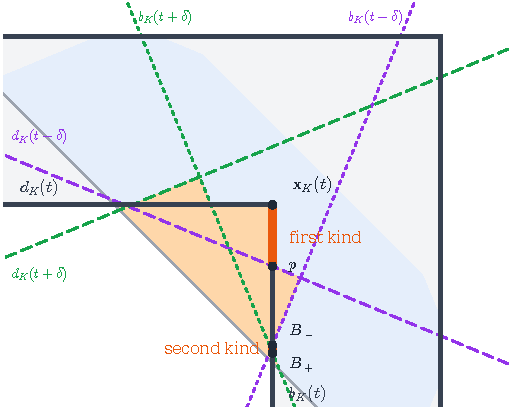
\includegraphics[width=0.8\linewidth]{figures/fig-wall}
\caption{\cref{lem:wall,lem:tau}, for the polygon cap with the angle set $\Theta_1$ ($n=4$, $\delta=\pi/8$) and the support values of Gerver's cap, at $t=\pi/4$, drawn in the frame of the supporting hallway $L_K(t)$ (the polygon niche is shaded). The part of $\vec b_K(t)$ above the dashed line $d_K(t-\delta)$ is the segment $[p,\xx_K(t)]$ (points of the first kind); further down $\vec b_K(t)$ runs between the dotted lines $b_K(t-\delta)$ and $b_K(t+\delta)$, from $B_-$ to $B_+$ (points of the second kind). The side of the niche on $\vec b_K(t)$ lies in the union of the two segments.}
\label{fig:wall}
\end{figure}

\begin{lemma}[with a defect]\label{lem:curv-defect}
Let $K\in\Kc_k$, $t\in\Theta_k$, $e\ge0$, $D\ge0$ with $g_K^+(t)\le D$ and $\sigma_K(t)\le\tau_K(t)+e$. Then
\[
  \sigma_K(t)\le k_0\bigl(g_K^+(t)\bigr)\,\delta+(D+4)\delta^2+e .
\]
\end{lemma}

\begin{proof}
Let $M=\abs{g_K^+(t)-1}\le D+1$. As $0\le g_K^-\le g_K^+$, each of $g_K^--1+q$ and $1-g_K^++q$ is at most $M+q$, so the first maximum
in \cref{lem:tau} is at most $\tan\delta\,(M+q)\le\delta M+(D+3)\delta^2$, using $\tan\delta\le\delta+\delta^2$, $q\le\delta$ and
$\delta\le1$. If $\sigma_K(t)\ge2q$, the second maximum is $0$ and
$\sigma_K(t)\le\tau_K(t)+e\le\delta M+(D+3)\delta^2+e$. If $\sigma_K(t)<2q$, then
$\sigma_K(t)\le\delta M+(D+3)\delta^2+(2q-\sigma_K(t))+e$ and $2q\le\delta+\delta^2$, so
$\sigma_K(t)\le\frac{M+1}2\delta+\frac{D+4}2\delta^2+\frac e2$. Both $M$ and $(M+1)/2$ are at most $k_0(g_K^+(t))$.
\end{proof}

\subsection{From normals to intervals}

\begin{lemma}[arms between two steps]\label{lem:cell}
Let $K\in\Kc_k$ have diameter at most $D$, and let $t\in\{0\}\cup\Theta_k$. Then $g_K^+$ is nonincreasing on
$[t,t+\delta)$, and $g_K^+(t)-g_K^+(u)\le D\delta$ for $u\in(t,t+\delta)$.
\end{lemma}

This is \baek{Lemma~6.4.1}, with $D$ in place of the bound $5$ for maximum polygon caps. The half-open interval is needed: $g_K^+$ jumps up at $t+\delta$, by $\sigma_K(t+\delta+\pi/2)$, and Baek's statement compares $g_K^+(t)$ with $g_K^-(t+\delta)$.

\begin{proof}
Since there is no normal angle of $K$ strictly between $t$ and $t+\delta$, nor between $t+\pi/2$ and
$t+\delta+\pi/2$, there are vertices $A$ and $C$ of $K$ with $A_K^\pm(s)=A$ and $C_K^\pm(s)=C$ for
$s\in(t,t+\delta)$, and also $A_K^+(t)=A$, $C_K^+(t)=C$. As $\yy_K(s)$ lies on $l_K(s)\ni A$, we get
$g_K^+(s)=\ip{A-C}{u_s}$ on $[t,t+\delta)$. Its derivative is $\ip{A-C}{v_s}$. It is at most $0$,
because $\ip A{v_s}\le h_K(s+\pi/2)=\ip C{v_s}$, and at least $-\norm{A-C}\ge-D$.
\end{proof}

\begin{lemma}[summing the steps]\label{lem:sum}
Let $K\in\Kc_k$ have diameter at most $D$ with $k_0(g_K^+)\le B$ on $[0,\pi/2]$, and suppose that for some $C\ge0$ and every
$t\in\{0\}\cup\Theta_k$
\[
  \sigma_K(t)\le k_0(g_K^+(t))\,\delta+C\delta^2+e(t),\qquad e(t)\ge0 .
\]
Then for $-\pi/2\le a<b\le\pi/2$ with $a'=\max(a,0)\le b$,
\[
  \sigma_K\bigl((a,b)\bigr)\le\int_{a'}^bk_0\bigl(g_K^+(u)\bigr)\dd u+\Bigl(B+\frac\pi2(C+D)\Bigr)\delta+\sum_{j=0}^{n-1}e(j\delta).
\]
\end{lemma}

\begin{proof}
On $(-\pi/2,\pi/2)$, $\sigma_K$ is carried by the points $j\delta$, $1\le j\le n-1$. For $t=j\delta$,
$0\le j\le n-1$, \cref{lem:cell}, together with $k_0$ being $1$-Lipschitz, gives
$k_0(g_K^+(t))\delta\le\int_t^{t+\delta}k_0(g_K^+)+D\delta^2$, so
$\sigma_K(t)\le\int_t^{t+\delta}k_0(g_K^+)+(C+D)\delta^2+e(t)$. Sum over the grid points $t\in[a',b)$; they
are at most $n$ in number, their cells $[t,t+\delta)$ lie in $[a',b+\delta)$ and the part beyond $b$ is shorter than $\delta$,
where $k_0(g_K^+)\le B$. Also $n(C+D)\delta^2=\frac\pi2(C+D)\delta$.
\end{proof}

The next two lemmas are the passage to the limit in the proof of \baek{Thm.~6.4.3}. Baek gets the lower semicontinuity of the mass of an open interval from the weak convergence of
$\sigma_{K_n}$ and the Portmanteau theorem; Lemma~\ref{lem:lsc} replaces this by a direct argument with support functions.

\begin{lemma}[lower semicontinuity of the mass of an open interval]\label{lem:lsc}
If convex bodies $K_j\to K$ in $\dH$ and $a<b$, then $\sigma_K((a,b))\le\liminf_j\sigma_{K_j}((a,b))$.
\end{lemma}

\begin{proof}
For $0<\eps<\pi$ let $\Phi_K(\eps)=\ip{v_K(b-\eps,b)}{v_b}-\ip{v_K(a,a+\eps)}{v_a}+\int_a^bh_K$. A point
$p=h_K(b)u_b+mv_b$ of $e_K(b)$ lies in $H_K(b-\eps)$, i.e. $h_K(b)\cos\eps-m\sin\eps\le h_K(b-\eps)$, so
$\ip{v_K^-(b)}{v_b}\ge\ip{v_K(b-\eps,b)}{v_b}$; likewise $\ip{v_K^+(a)}{v_a}\le\ip{v_K(a,a+\eps)}{v_a}$. By
\eqref{eq:sigma-open}, $\Phi_K(\eps)\le\sigma_K((a,b))$, and $\Phi_K(\eps)\to\sigma_K((a,b))$ as $\eps\downarrow0$ by
\cref{fact:convex}\ref{fact:convex:vertices}. For fixed $\eps$, $\Phi_{K_j}(\eps)\to\Phi_K(\eps)$, as $\Phi$ is an explicit
continuous function of the support function. Hence
$\sigma_K((a,b))=\lim_\eps\lim_j\Phi_{K_j}(\eps)\le\liminf_j\sigma_{K_j}((a,b))$.
\end{proof}

\begin{lemma}[passing to the limit]\label{lem:limit}
Let $K_j$ be polygon caps with rotation angle $\pi/2$ that converge in $\dH$ to $K\in\Kc_{\pi/2}$, and let $\eps_j\to0$
be such that, for all $-\pi/2\le a<b\le\pi/2$ with $a'=\max(a,0)\le b$,
\[
  \sigma_{K_j}\bigl((a,b)\bigr)\le\int_{a'}^bk_0\bigl(g_{K_j}^+\bigr)+\eps_j .
\]
Then $\sigma_K(E)\le\int_Ek_0(g_K^+(t))\dd t$ for every Borel set $E\subset[0,\pi/2)$.
\end{lemma}

\begin{proof}
By \cref{fact:iteration}\ref{fact:iteration:arms} and since $k_0$ is $1$-Lipschitz,
$\int_{a'}^bk_0(g_{K_j}^+)\to\int_{a'}^bk_0(g_K^+)$. With \cref{lem:lsc},
$\sigma_K((a,b))\le\int_{a'}^bk_0(g_K^+)$ for all such $a<b$. A nonempty relatively open interval of $[0,\pi/2)$ is $(a,b)$ with $a\ge0$, or $[0,b)\subset(a,b)$ for every
$a\in[-\pi/2,0)$, so the inequality $\sigma_K(E)\le\int_Ek_0(g_K^+)$ holds for every such interval $E$, hence for every relatively open set, and by outer regularity of
the finite measure $k_0(g_K^+)\dd t$ for every Borel set.
\end{proof}

\subsection{The curvature bounds}

\begin{definition}[curvature bounds]\label{def:curvature}
A cap $K\in\Kc_{\pi/2}$ satisfies the \emph{curvature bounds} if, as measures,
\[
  \sigma_K\le k_0\bigl(g_K^+(t)\bigr)\dd t\ \text{ on }[0,\pi/2),\qquad
  \sigma_K\le k_0\bigl(f_K^-(t-\pi/2)\bigr)\dd t\ \text{ on }(\pi/2,\pi].
\]
\end{definition}

\begin{proposition}[maximizing caps satisfy the curvature bounds]\label{prop:curvature}
Every maximizing cap $K_*\in\Kc_{\pi/2}$ with $\cA(K_*)>0$ satisfies the curvature bounds.
\end{proposition}

\begin{proof}
Take the selection $K_j\to K_*$ of \cref{prop:selection}, with stages $k_j$, step sizes $\delta_j\to0$, in
$[-R_0,R_0]\times[0,1]$, and $\eta_j=\dH(K_j,K_*)\to0$. The diameter of $K_j$ is at most $D=2R_0+1$; so
$g_{K_j}^+\le D$ and $k_0(g_{K_j}^+)\le B=D+1$. For $t\in\Theta_{k_j}$, \cref{prop:floating} gives
$\sigma_{K_j}(t)\le\tau_{K_j}(t)+e_j(t)$ with $e_j(t)=2\eta_j\nu_{k_j}(t)\ge0$, so by \cref{lem:curv-defect}
\[
  \sigma_{K_j}(t)\le k_0(g_{K_j}^+(t))\delta_j+(D+4)\delta_j^2+e_j(t).
\]
At $t=0$ this holds trivially, since $\sigma_{K_j}(0)=0$ (put $e_j(0)=0$). By \cref{lem:sum} with $C=D+4$,
for $-\pi/2\le a<b\le\pi/2$ with $a'\le b$,
\[
  \sigma_{K_j}((a,b))\le\int_{a'}^bk_0(g_{K_j}^+)+\bigl(B+\pi(D+2)\bigr)\delta_j+2\eta_j,
\]
since the weights at distinct normals add up to less than $1$, \eqref{eq:weights}, so $\sum_te_j(t)\le2\eta_j$.
By \cref{lem:limit}, $K_*$ satisfies the first curvature bound. The reflection $K_*^{\mir}$ is a cap with the same sofa area
(\cref{fact:monotone}\ref{fact:monotone:mirror}), hence maximizing with positive sofa area; by
\cref{fact:arms}\ref{fact:arms:mirror} and $\sigma_{K^{\mir}}(E)=\sigma_K(\pi-E)$, its first bound is the second bound
for $K_*$.
\end{proof}

\begin{figure}[ht]
\centering
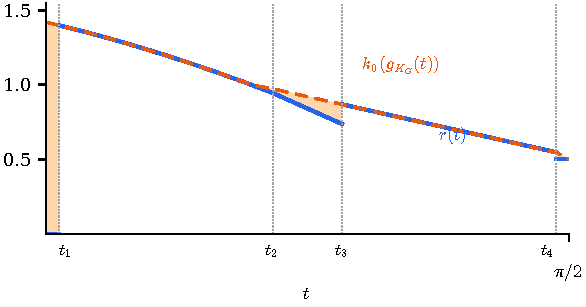
\includegraphics[width=0.78\linewidth]{figures/fig-curvature}
\caption{The first curvature bound for Gerver's cap, which maximizes $\cA$ (\cref{fact:optimal}): the density $r(t)$ of $\sigma_{\KG}$ on $[0,\pi/2)$ (blue) lies
below $k_0(g_{\KG}(t))$ (orange, dashed), computed from Romik's rotation path. They agree on $[t_1,t_*]$, where $g_{\KG}(t_*)=2$ ($t_*=0.616\ldots$), and on $[t_3,t_4]$; the gap is shaded.}
\label{fig:curvature}
\end{figure}

\subsection{The injectivity condition}

\begin{lemma}[integral inequalities]\label{lem:integral}
Let $K\in\Kc_{\pi/2}$ satisfy the curvature bounds. Then $K$ satisfies condition (1) of \cref{def:inj}, and
\begin{gather*}
  f_K(t)-1\ge\int_0^tm_0\bigl(g_K(u)\bigr)\dd u\quad(0\le t<\tfrac\pi2),\\
  g_K(t)-1\ge\int_t^{\pi/2}m_0\bigl(f_K(u)\bigr)\dd u\quad(0<t\le\tfrac\pi2).
\end{gather*}
\end{lemma}

\begin{proof}
Each restriction of $\sigma_K$ is dominated by a finite measure with a density, so it has a density
(Radon--Nikodym) and condition (1) holds. By \cref{fact:arms}\ref{fact:arms:regular}, $f_K,g_K$ are defined and continuous, $f_K(0)=1$, and
by \cref{fact:arms}\ref{fact:arms:integral}, for $t<\pi/2$,
$f_K(t)-1=\int_0^tg_K-\sigma_K((0,t])\ge\int_0^t(g_K-k_0(g_K))=\int_0^tm_0(g_K)$. For the second inequality apply the first to the
reflection $K^{\mir}$, which satisfies the curvature bounds with their roles exchanged, and use
\cref{fact:arms}\ref{fact:arms:mirror}: $f_{K^{\mir}}(s)=g_K(\pi/2-s)$ and $g_{K^{\mir}}(s)=f_K(\pi/2-s)$, with $t=\pi/2-s$.
\end{proof}

\begin{lemma}[the lower sequence]\label{lem:lower}
Let $f,g:[0,\pi/2]\to[0,\infty)$ be continuous with $f(t)-1\ge\int_0^tm_0(g)$ for $t\in[0,\pi/2)$ and
$g(t)-1\ge\int_t^{\pi/2}m_0(f)$ for $t\in(0,\pi/2]$. Then for every $j\ge0$, $f_j(t)\le f(t)$ on $[0,\pi/2)$ and
$f_j(\pi/2-t)\le g(t)$ on $(0,\pi/2]$.
\end{lemma}

\begin{proof}
Induction on $j$, the case $j=0$ being $f_0=0\le f,g$. If it holds for $j$, then for $t\in[0,\pi/2)$, since $m_0$ is
nondecreasing and $f_j(\pi/2-u)\le g(u)$ for $u\in(0,t]$,
$\mathcal Ff_j(t)=1+\int_0^tm_0(f_j(\pi/2-u))\dd u\le1+\int_0^tm_0(g)\le f(t)$, and with $f_j\le f$ we get
$f_{j+1}=\max(f_j,\mathcal Ff_j)\le f$ on $[0,\pi/2)$. For $t\in(0,\pi/2]$,
$\mathcal Ff_j(\pi/2-t)=1+\int_t^{\pi/2}m_0(f_j(s))\dd s\le1+\int_t^{\pi/2}m_0(f)\le g(t)$, and with
$f_j(\pi/2-t)\le g(t)$ this gives $f_{j+1}(\pi/2-t)\le g(t)$.
\end{proof}

\begin{proposition}[injectivity]\label{prop:inj}
Every $K\in\Kc_{\pi/2}$ that satisfies the curvature bounds satisfies the injectivity condition, and
$f_K,g_K>1$ on $(0,\pi/2)$.
\end{proposition}

\begin{proof}
By \cref{lem:integral}, $K$ satisfies (1) and the integral inequalities, and $f_K,g_K$ are continuous and nonnegative.
By \cref{lem:lower} and \cref{fact:iteration}\ref{fact:iteration:eleven}, for $t\in(0,\pi/2)$,
$1<f_{11}(t)\le f_K(t)$ and $1<f_{11}(\pi/2-t)\le g_K(t)$. By \cref{fact:arms}\ref{fact:arms:regular}, $\xx_K$ is continuously differentiable with
$\xx_K'=-(f_K-1)u_t+(g_K-1)v_t$, which gives (2) and (3).
\end{proof}

\begin{corollary}[maximizing right-angle caps are in $\Ki$]\label{cor:Ki}
Every $K\in\Kc_{\pi/2}$ with $\cA(K)=\abs\Gs$ lies in $\Ki$.
\end{corollary}

\begin{proof}
$K$ is maximizing (\cref{fact:optimal}) and $\cA(K)=\abs\Gs>0$, so it satisfies the curvature bounds
(\cref{prop:curvature}) and the injectivity condition (\cref{prop:inj}); and $\abs K\ge\cA(K)=\abs\Gs\ge11/5$.
\end{proof}

\section{Equality in Baek's upper bound}\label{sec:equality}

Let $K\in\Kc_{\pi/2}$ with $\cA(K)=\abs\Gs$. By \cref{cor:Ki}, $K\in\Ki$. Write $K_0=\KG$ for Gerver's cap, $K_1=K$,
$h_i=h_{K_i}$ and $\Delta=h_1-h_0$; since both are caps with rotation angle $\pi/2$, $\Delta(\pi/2)=0$. Let
$\xi_0=\xi_G$ and $\xi_1=\xi_K$ be the canonical triples (\cref{sec:Q}), and $K_{1/2}$, $B_{1/2}$, $D_{1/2}$ the components of
$\xi_{1/2}=\tfrac12\xi_0+\tfrac12\xi_1$.

\subsection{Equality in the concavity of \texorpdfstring{$\cQ$}{Q}}

\begin{lemma}[equality in \texorpdfstring{$\cS$}{S}]\label{lem:equality}
For each of the four terms $\cM_K(a,b;\mathbf z_K)$ of $\cS_K$,
\[
  \cM_{K_{1/2}}\bigl(a,b;\mathbf z_{K_{1/2}}\bigr)=\tfrac12\cM_{K_0}\bigl(a,b;\mathbf z_{K_0}\bigr)+\tfrac12\cM_{K_1}\bigl(a,b;\mathbf z_{K_1}\bigr).
\]
\end{lemma}

\begin{proof}
By \cref{fact:Q}\ref{fact:Q:triple}, \ref{fact:Q:max}, $\abs\Gs=\cA(K)\le\cQ(\xi_1)\le\abs\Gs$, and
$\cQ(\xi_0)=\abs\Gs$, so $\cQ(\xi_0)=\cQ(\xi_1)=\abs\Gs$. The set $\cT$ is closed under Minkowski combinations, so $\xi_{1/2}\in\cT$.
By \cref{fact:Q}\ref{fact:Q:decomp},
$\cQ=\Lambda-\cS-\cR-\cL$ with $\Lambda$ convex-linear and the three terms convex, so $\cQ(\xi_{1/2})\ge\frac12\cQ(\xi_0)+\frac12\cQ(\xi_1)=\abs\Gs$, while
$\cQ(\xi_{1/2})\le\abs\Gs$ by \cref{fact:Q}\ref{fact:Q:max}. So equality holds, and since $\Lambda$ is convex-linear this says
\[
  \bigl[\cS_{K_{1/2}}-\tfrac12\cS_{K_0}-\tfrac12\cS_{K_1}\bigr]+\bigl[\cR_{B_{1/2}}-\tfrac12\cR_{B_0}-\tfrac12\cR_{B_1}\bigr]
  +\bigl[\cL_{D_{1/2}}-\tfrac12\cL_{D_0}-\tfrac12\cL_{D_1}\bigr]=0 .
\]
Each bracket is $\le0$ by convexity, so each is $0$. The first is the sum of the corresponding brackets of
the four terms of $\cS$, which are all $\le0$; so each of them is $0$.
\end{proof}

\subsection{Equal tangent displacements}

By \cref{fact:Q}\ref{fact:Q:decomp}, for each term the displacement $\varrho_{K,\mathbf z_K}(t)$ is convex-linear in $K$. Write
$\varrho_i=\varrho_{K_i,\mathbf z_{K_i}}$, so that $\varrho_{1/2}=\frac12(\varrho_0+\varrho_1)$ and
\[
  \tfrac12\varrho_0^2+\tfrac12\varrho_1^2-\varrho_{1/2}^2=\tfrac14(\varrho_0-\varrho_1)^2 .
\]
So the equality of \cref{lem:equality} reads
\begin{equation}\label{eq:gap}
  \tfrac18\int_a^b\bigl(\varrho_0(t)-\varrho_1(t)\bigr)^2\dd t=0 ,
\end{equation}
and $\varrho_0=\varrho_1$ almost everywhere on $[a,b]$. The four intervals are $(0,\varphi)$, $(\varphi,\pi/2-\varphi)$,
$(\pi/2-\varphi,\pi/2)$ and $(\pi/2,\pi)$; none contains $\pi/2$. On each of them both $K_i$ satisfy
condition~(1) of the injectivity condition, so by \cref{fact:arms}\ref{fact:arms:regular} the vertices $v^+_{K_i}$ and $v^-_{K_i}$
agree there, and by \cref{fact:convex}\ref{fact:convex:vertices} (one-sided continuity) they are continuous there; so $h_i$ is differentiable with the continuous derivative $h_i'(t)=\ip{v^+_{K_i}(t)}{v_t}$,
and $\varrho_0,\varrho_1$ are continuous. Hence $\varrho_0=\varrho_1$ \emph{everywhere} on $(a,b)$. We read this off for the two kinds of curves.

\begin{lemma}[the tangent equations]\label{lem:tangent}
Let $(a,b)$ be one of the four intervals.
\begin{enumerate}[label=(\alph*)]
\item\label{lem:tangent:l} Suppose that $\mathbf z_K=\mathbf l_K^T$ with $b\le T<a+\pi$. Then there are $p,q\in\R$ with
$\Delta(t)=p\cos t+q\sin t$ for $t\in[a,b]$, and $\Delta(T)=p\cos T+q\sin T$.
\item\label{lem:tangent:y} Suppose that $\mathbf z_K=\yy_K$ (the second term, $(a,b)=(\varphi,\pi/2-\varphi)$). Then
$\Delta(t)=\Delta(b)-\int_t^b\Delta(u+\pi/2)\dd u$ for $t\in[a,b]$.
\end{enumerate}
\end{lemma}

\begin{proof}
\ref{lem:tangent:l} For $t\in(a,b)$ we have $0<T-t<\pi$, and $\ip{\mathbf l_K^T(t)}{v_t}=(h_K(T)-h_K(t)\cos(T-t))/\sin(T-t)$, so
$\varrho_i(t)=\dfrac{h_i(T)-h_i(t)\cos(T-t)}{\sin(T-t)}-h_i'(t)$. The equality $\varrho_0=\varrho_1$ is
\[
  \sin(T-t)\Delta'(t)+\cos(T-t)\Delta(t)=\Delta(T).
\]
Then $\chi(t)=\bigl(\Delta(t)-\Delta(T)\cos(T-t)\bigr)/\sin(T-t)$ has $\chi'=\bigl[\Delta'\sin(T-t)+\Delta\cos(T-t)-\Delta(T)\bigr]/\sin^2(T-t)=0$ on $(a,b)$, so
$\chi\equiv\kappa$ and $\Delta(t)=\Delta(T)\cos(T-t)+\kappa\sin(T-t)=p\cos t+q\sin t$, with $p=\Delta(T)\cos T+\kappa\sin T$ and
$q=\Delta(T)\sin T-\kappa\cos T$; then $p\cos T+q\sin T=\Delta(T)$. By continuity this holds on $[a,b]$.

\ref{lem:tangent:y} Here $\ip{\yy_K(t)-v^+_K(t)}{v_t}=h_K(t+\pi/2)-h_K'(t)$, so $\varrho_0=\varrho_1$ says $\Delta'(t)=\Delta(t+\pi/2)$ on $(a,b)$. Integrate; $\Delta$ is continuous.
\end{proof}

\subsection{The cap is a horizontal translate}

\begin{proposition}[the difference of support functions]\label{prop:kernel}
$\Delta(t)=s\cos t$ for $t\in[0,\pi]$, where $s=-\Delta(\pi)$.
\end{proposition}

\begin{proof}
We solve the four equations in reverse order, using $\Delta(\pi/2)=0$.

On $[\pi/2,\pi]$ (target $T=\pi$): $\Delta=p\cos t+q\sin t$ and $\Delta(\pi/2)=q=0$, so $\Delta(t)=p\cos t$ and $\Delta(\pi)=-p$; thus
$\Delta(t)=s\cos t$ on $[\pi/2,\pi]$ with $s=-\Delta(\pi)$.

On $[\pi/2-\varphi,\pi/2]$ (target $T=\pi-\varphi$): $\Delta=p'\cos t+q'\sin t$, $\Delta(\pi/2)=q'=0$, and $\Delta(\pi-\varphi)=p'\cos(\pi-\varphi)$.
By the previous step $\Delta(\pi-\varphi)=s\cos(\pi-\varphi)$, and $\cos(\pi-\varphi)\ne0$, so $p'=s$.

On $[\varphi,\pi/2-\varphi]$: with $b=\pi/2-\varphi$, $\Delta(u+\pi/2)=s\cos(u+\pi/2)=-s\sin u$ for $u\in[\varphi,b]$ by the first
step, and $\Delta(b)=s\cos b$ by the second, so
$\Delta(t)=s\cos b+s\int_t^b\sin u\dd u=s\cos t$.

On $[0,\varphi]$ (target $T=\pi/2$): $\Delta=p''\cos t+q''\sin t$, $\Delta(\pi/2)=q''=0$, and $\Delta(\varphi)=s\cos\varphi=p''\cos\varphi$ gives $p''=s$.
\end{proof}

\begin{figure}[ht]
\centering
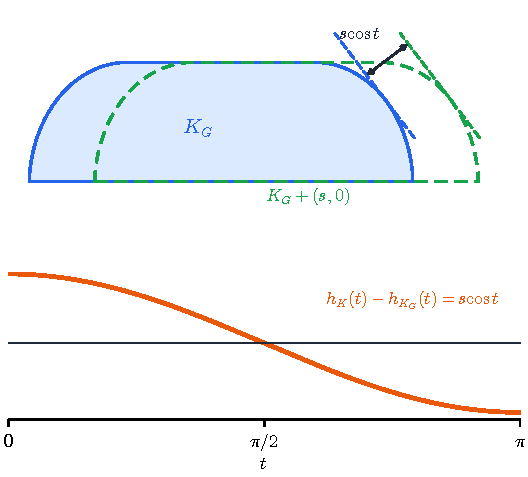
\includegraphics[width=0.74\linewidth]{figures/fig-translate}
\caption{\cref{prop:kernel,lem:translate}. Top: Gerver's cap $K_G$ and its horizontal translate by $(s,0)$; their supporting lines at the normal $t$
lie $s\cos t$ apart. Bottom: the difference $h_K-h_{K_G}=s\cos t$ of the support functions on $[0,\pi]$.}
\label{fig:translate}
\end{figure}

\begin{lemma}[caps with translated supports]\label{lem:translate}
If $K,C\in\Kc_{\pi/2}$ and $h_K(t)-h_C(t)=s\cos t$ for $t\in[0,\pi]$, then $K=C+(s,0)$ and
$K\setminus\cN(K)=(C\setminus\cN(C))+(s,0)$.
\end{lemma}

\begin{proof}
By \eqref{eq:cap-fan} with $\omega=\pi/2$, $K=\{p:\,p_y\ge0,\ \ip p{u_t}\le h_K(t)\text{ for }t\in[0,\pi]\}$, and likewise for $C$.
Since $h_{C+(s,0)}(t)=h_C(t)+s\cos t$ and $(s,0)$ is parallel to the floor, $C+(s,0)$ is the same set as $K$.
Finally $Q^-_{C+w}(t)=Q^-_C(t)+w$ and $F_{\pi/2}+(s,0)=F_{\pi/2}$.
\end{proof}

\begin{theorem}[maximizing right-angle caps]\label{thm:caps}
A cap $K\in\Kc_{\pi/2}$ has $\cA(K)=\abs\Gs$ if and only if $K=\KG+(s,0)$ for some $s\in\R$. In this case
$K\setminus\cN(K)=\Gs+(s,0)$. Consequently the maximizers of $\cA$ on $\Kc_{\pi/2}$ are the horizontal translates of Gerver's cap, and
every monotone sofa $U$ with rotation angle $\pi/2$ and $\abs U=\abs\Gs$ is a horizontal translate of $\Gs$.
\end{theorem}

\begin{proof}
If $\cA(K)=\abs\Gs$, then $K\in\Ki$ by \cref{cor:Ki}; \cref{prop:kernel} and \cref{lem:translate} (with $C=\KG$)
give $K=\KG+(s,0)$ and $K\setminus\cN(K)=(\KG\setminus\cN(\KG))+(s,0)=\Gs+(s,0)$ by \cref{fact:gerver}\ref{fact:gerver:cap}.
Conversely $\cA(\KG)=\abs\Gs$ by \cref{fact:monotone}\ref{fact:monotone:area}, and $\cA(C+(s,0))=\cA(C)$ for every cap $C$, since
$\cN(C+(s,0))=\cN(C)+(s,0)$. The maximum of $\cA$ is $\abs\Gs$ by \cref{fact:optimal}. If $U$ is a monotone
sofa with rotation angle $\pi/2$ and $\abs U=\abs\Gs$, its cap $K=\cC(U)$ has $\cA(K)=\abs U=\abs\Gs$
(\cref{fact:monotone}\ref{fact:monotone:area}), and $U=K\setminus\cN(K)$.
\end{proof}

\section{Recovering the sofa; proof of Theorem~\ref{thm:main}}\label{sec:recovery}

By \eqref{eq:contained} and \cref{thm:caps}, a rigid image of $S$ lies in a horizontal translate of $\Gs$ and has
the same area. A closed subset of a set of finite area, with the same area, is the whole set if that set
is the closure of its interior (\cref{lem:recover}), but not in general (\cref{fig:recovery}, Remark~\ref{rem:needed}). So it remains to show that $\Gs$ is.

\begin{lemma}[recovering a set from its area]\label{lem:recover}
Let $X\subset Y\subset\R^2$ with $X$ closed, $Y=\clos(\inter Y)$, $\abs Y<\infty$ and $\abs X=\abs Y$. Then $X=Y$.
\end{lemma}

\begin{proof}
$\abs{Y\setminus X}=0$. The set $\inter Y\setminus X$ is open, and it has measure $0$, so it is empty. Hence
$\inter Y\subset X$, and since $X$ is closed, $Y=\clos(\inter Y)\subset X$.
\end{proof}

\begin{remark}\label{rem:needed}
Both hypotheses on $Y$ are needed. The closed connected set $Y=[0,1]^2\cup([1,2]\times\{0\})$ and its closed
subset $X=[0,1]^2$ have the same finite area, and $Y$ is not the closure of its interior. For $Y=\R^2$ and $X=\R^2$ minus the open unit disc, $Y=\clos(\inter Y)$ and
$\abs X=\abs Y=\infty$. For $Y=\Gs$, a closed subset that misses an interior point of $\Gs$ misses a disc about it, and so loses area.
\end{remark}

\begin{lemma}[removing the region under an envelope]\label{lem:envelope}
Let $K\subset\R^2$ be closed with $K=\clos(\inter K)$ and $[a,b]\times[0,1]\subset K$. Let $\Gamma$ be a compact set of points with
abscissa in $[a,b]$ and height in $[0,1)$, and let $\Gamma_<$ be the set of points $q$ with $q_y\ge0$ that lie strictly
below a point $\gamma$ of $\Gamma$ with $\gamma_x=q_x$. If $X=K\setminus\Gamma_<$ is closed, then $X=\clos(\inter X)$.
\end{lemma}

\begin{proof}
Let $\bar\Gamma$ be the set of points $q$ with $q_y\ge0$ that lie on or below a point of $\Gamma$ with the same abscissa; it
is the image of the compact set $\Gamma\times[0,1]$ under $(\gamma,\lambda)\mapsto(\gamma_x,\lambda\gamma_y)$, hence compact, and
$\Gamma_<\subset\bar\Gamma$. Let $p\in X$.

If $p\notin\bar\Gamma$, then $p$ has a neighborhood outside $\bar\Gamma$, and since $K=\clos(\inter K)$ it is a limit of interior
points of $K$ outside $\bar\Gamma$; these are interior points of $X=K\setminus\Gamma_<$. So $p\in\clos(\inter X)$.

If $p\in\bar\Gamma$, then $p\notin\Gamma_<$ means that $p$ is the highest point of $\Gamma$ on its vertical line: $p_x\in[a,b]$ and
$p_y<1$. The points $(p_x,p_y+s)$, $0<s\le1-p_y$, lie in the rectangle $[a,b]\times[0,1]\subset K$ and outside $\bar\Gamma$, so by the
first case they lie in $\clos(\inter X)$, and so does their limit $p$.

So $X\subset\clos(\inter X)$, and $\clos(\inter X)\subset X$ since $X$ is closed.
\end{proof}

\begin{proposition}[Gerver's sofa is regular closed]\label{prop:regular}
$\Gs=\clos(\inter\Gs)$.
\end{proposition}

\begin{proof}
Let $\Gamma=\bD([t_0,t_2])\cup\xx([t_1,t_4])\cup\bB([t_3,t_5])$, $a=\bD(0)_x$ and $b=\bB(\pi/2)_x$. By
\cref{fact:gerver}\ref{fact:gerver:cap} and~\ref{fact:gerver:niche}, $\Gs=\KG\setminus\cN(\KG)=\KG\setminus\Gamma_<$, which is closed, being a moving sofa.
The set $\Gamma$ is compact. The abscissa increases along $\bD$ and $\bB$ and, as $t$ grows, decreases along $\xx$, and the
endpoints are joined, so
\[
  a=\bD(0)_x<\bD(t_2)_x=\xx(t_4)_x<\xx(t_1)_x=\bB(t_3)_x<\bB(t_5)_x=b ,
\]
and the abscissa of every point of $\Gamma$ lies in $[a,b]$. The ordinate of $\bD$ is nondecreasing, since
$\bD'$ is a positive multiple of $u_t$ and $\sin t\ge0$; it starts at $0$ and ends at $\xx(t_4)_y<1$. The ordinate of $\bB$ is
nonincreasing, since $\bB'$ is a negative multiple of $v_t$; it ends at $0$ and starts at $\xx(t_1)_y<1$. The ordinate of $\xx$ on
$[t_1,t_4]$ lies in $(0,1)$ by \cref{fact:height}. So the heights of $\Gamma$ lie in $[0,1)$.

The points $(a,1)=\bD(0)+v_0=\bC(0)$ and $(b,1)=\bB(\pi/2)+u_{\pi/2}=\bA(\pi/2)$ are vertices of the cap $\KG$ (\cref{fact:gerver}\ref{fact:gerver:cap}), so they lie in $\KG$.
A cap with rotation angle $\pi/2$ is closed downward above the floor: for $p\in K$ and $0\le\lambda\le p_y$ we have $p-(0,\lambda)\in K$,
because $\ip{(0,-\lambda)}{u_s}\le0$ for $s\in[0,\pi]$. Hence $\KG\supset[a,b]\times[0,1]$, so $\KG$ is a closed convex set with nonempty interior, and
$\KG=\clos(\inter\KG)$. \cref{lem:envelope} applies with $K=\KG$.
\end{proof}

\begin{figure}[ht]
\centering
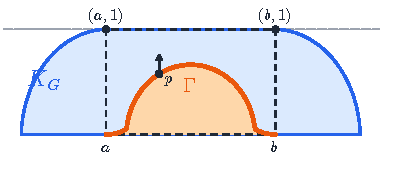
\includegraphics[width=0.92\linewidth]{figures/fig-recovery}
\caption{\cref{prop:regular}. Left: Gerver's cap $\KG$ with its niche (orange) below the curve $\Gamma$ formed by $\bD$, $\xx$ and $\bB$; the dashed rectangle
$[a,b]\times[0,1]$ lies in $\KG$, and the greatest height of $\Gamma$ is $0.664\ldots$. Every point $p$ of $\Gamma$ is a limit of points of
$\Gs$ above it. Right: why $\clos(\inter Y)=Y$ is needed in \cref{lem:recover}: a closed subset of $Y$ with the same area misses
no interior point.}
\label{fig:recovery}
\end{figure}

\begin{proof}[Proof of \cref{thm:main}]
Let $S$ be a moving sofa with $\abs S=\abs\Gs$. By \cref{prop:reduction}, \cref{prop:U} and \cref{thm:caps}, there are $\omega\in[\omega_0,\pi/2]$,
$\psi=\pi/2-\omega$, $w_0,w_1\in\R^2$ and $s\in\R$ such that
\[
  g_1(S)\subset U=\Gs+(s,0),\qquad g_1(p)=R_\psi(p+w_0)+w_1 .
\]
Let $g(p)=g_1(p)-(s,0)=R_\psi p+v$ with $v=R_\psi w_0+w_1-(s,0)$. Then $g(S)\subset\Gs$. The set $g(S)$ is closed, since $S$ is closed and $g$ is a
homeomorphism, and $\abs{g(S)}=\abs S=\abs\Gs<\infty$ since $g$ preserves area. By \cref{prop:regular}, $\Gs=\clos(\inter\Gs)$, so
$g(S)=\Gs$ by \cref{lem:recover}, that is, $R_\psi S+v=\Gs$. This is the assertion with $\theta=\psi$.
\end{proof}

The proof also gives the following description of all maximal sofas.

\begin{corollary}[the maximal sofas]\label{cor:all}
A set $S$ is a moving sofa of maximal area if and only if it is a moving sofa and $R_\theta S+v=\Gs$ for some $\theta$ and $v$.
\end{corollary}

\begin{proof}
One direction is \cref{thm:main} together with $\abs S=\abs\Gs$ being the maximum (\cref{fact:optimal}). Conversely a rigid image of $\Gs$ has the area of $\Gs$.
\end{proof}

\begin{remark}[no rotation is needed]\label{rem:translate}
In \cref{thm:main} one can take $\theta=0$: every moving sofa $S$ with $\abs S=\abs\Gs$ is a translate of $\Gs$, and so has the rotation angle $\pi/2$. This refinement is
not part of the formal statement. Indeed, a moving sofa lies after a translation in the strip $\R\times[0,1]$, so
$\abs{\ip{p-q}{u_{\pi/2}}}\le1$ for $p,q\in S$. In the proof above $\theta=\psi\in[0,\pi/2-\omega_0]$ and $S=R_{-\psi}(\Gs-v)$, so the width of $\Gs$ in the direction $u_{\pi/2+\psi}$ is at most one.
But the width of $\Gs$ in the direction $u_r$ exceeds one for every $r\in[0,\pi]\setminus\{\pi/2\}$, and $\pi/2+\psi\in[\pi/2,\pi)$; so $\psi=0$.

To see the claim about the width, let $a<b$ be as in \cref{prop:regular}, and let $x_-=\bC(\pi/2)_x$. The points $(a,1)=\bC(0)$ and $(b,1)=\bA(\pi/2)$ (the ends of the top edge of $\KG$), $(1,0)=\bA(0)$ (Appendix~\ref{app:gerver}, condition~(2))
and $(x_-,0)=\bC(\pi/2)$ (the ends of the floor, by \eqref{eq:ends}, \cref{fact:arms}\ref{fact:arms:regular} and \cref{fact:gerver}\ref{fact:gerver:cap}) lie in $\KG$, and not in $\cN(\KG)$: the points of $\cN(\KG)$ have height less than $1$ and abscissa in $(a,b)$ (the
only points of $\Gamma$ with abscissa $a$ or $b$ are $\bD(t_0)$ and $\bB(t_5)$, of height $0$), while $x_-=-h_{\KG}(\pi)\le a<b\le h_{\KG}(0)=1$. So they lie in $\Gs$.
For $r\in[0,\pi/2)$ the width of $\Gs$ in the direction $u_r$ is at least $\ip{(b,1)-(x_-,0)}{u_r}=(b-x_-)\cos r+\sin r>\cos r+\sin r\ge1$, because $b-x_->1$: indeed $x_-=\bC(\pi/2)_x=\xx(\pi/2)_x-1$, and
$b=\bB(t_5)_x>\bB(t_3)_x=\xx(t_1)_x>\xx(t_4)_x\ge\xx(\pi/2)_x$ by \cref{fact:gerver}\ref{fact:gerver:niche}.
For $r\in(\pi/2,\pi]$ it is at least $\ip{(a,1)-(1,0)}{u_r}=(1-a)\abs{\cos r}+\sin r>\abs{\cos r}+\sin r\ge1$, because $a<0$:
$a=\bD(t_0)_x<\bD(t_2)_x=\xx(t_4)_x<\xx(t_1)_x\le\xx(0)_x=0$ by \cref{fact:gerver}\ref{fact:gerver:niche} and Appendix~\ref{app:gerver}, condition~(2).
(Numerically, $a=-1.4206\ldots$, $b=0.1931\ldots$ and $x_-=-2.2275\ldots$.)
\end{remark}

\section{Quantitative stability}\label{sec:quant-stability-overview}

Write $M=\abs\Gs$ and $\eps(S)=M-\abs S$. Throughout this section distance
means Euclidean Hausdorff distance between the actual compact sets, not between
their convex hulls. For a nonempty compact set $S$, put
\[
 m(S)=\frac{h_S(0)-h_S(\pi)}2,
 \qquad
 S_c=S+\bigl(m(\Gs)-m(S),\,1-h_S(\pi/2)\bigr).
\]
This translation aligns the midpoints of the horizontal projections and the
upper supports. It differs from the left-support normalization $S^\natural$
used in the simpler stability proof in \cref{sec:stability}.

\begin{theorem}[explicit local stability; quantitative draft]
\label{thm:quant-explicit-stability}
There is $\eps_0>0$ such that every moving sofa $S$ with
$0\le\eps=\eps(S)<\eps_0$ satisfies
\[
 d_H(S_c,\Gs)\le\frac{23}{10}\sqrt\eps,
 \qquad
 \abs{S_c\triangle\Gs}\le50\sqrt\eps.
\]
Moreover, every admissible reduced motion of $S$ with total rotation
$\omega\in[\arccos(5/11),\pi/2]$ satisfies
\[
 0\le\frac\pi2-\omega\le\frac{31}{10}\eps.
\]
No smoothness, injectivity, or monotonicity of the input sofa is assumed.
\end{theorem}
\quantstatus{The exact statement is
\quantcode{MovingSofaQuantitative.Targets.ExplicitLocalStability}, with an
uncompiled theorem body in \quantcode{MovingSofaQuantitative.explicit_local_stability}.
The numerical sector, normal, terminal, and direct-area assemblies are present
in the quantitative library. None of these new modules has been compiled or
kernel checked; the integrated existential-coefficient theorem remains the
verified baseline \cref{thm:stability,thm:stability-angle}.}

The coefficient $23/10$ is an upper bound, not an optimal constant. The
threshold is initially left existential: this isolates the geometric content
of the square-root estimate from the effectivity calculations. The final
proposition of \cref{sec:quant-refinements} records the explicit common cutoff
$10^{-600}$; its uncompiled proof source is kept separate from this local proof.

\subsection{Why the square root occurs}

The starting point is Baek's upper-bound functional on the enlarged domain of
triples. For $\xi=(K,B,D)$, its deficit has an exact decomposition
\[
 M-\cQ(\xi)=L(\xi)+E_{\mathrm{cap}}(\xi)+E_B(\xi)+E_D(\xi),
 \qquad L,E_{\mathrm{cap}},E_B,E_D\ge0.
\]
Each energy is half an integral of a squared residual. Integrating the four
residual equations reconstructs the upper support of the cap, modulo a
horizontal translation. Cauchy--Schwarz therefore converts the energy into a
square-root support error. The simpler, left-pinned form is
\[
 d_H\bigl(K,\KG+(s_{\mathrm{left}},0)\bigr)
 \le 2\sec\varphi\sqrt{M-\cQ(\xi)}.
\]
This is \cref{thm:stability-cap}; its detailed proof is retained in
\cref{sec:stab-certificate,sec:stab-cap}. Centering the horizontal projection
instead of pinning one endpoint halves the coefficient to $\sec\varphi$;
\cref{thm:quant-centered-energy,thm:quant-centered-cap} give the refinement.

\subsection{From the cap back to the sofa}

Here is the proof architecture of \cref{thm:quant-explicit-stability}; the
technical estimates and numerical reductions are deferred to the appendices.
First, compactness and the uniqueness theorem place every sufficiently
near-optimal normalized sofa in a fixed neighborhood of Gerver's. The local
canonical construction then assigns a right-angle cap $K$ and its full-angle
envelope $U=K\setminus N(K)$. The construction gives
\[
 \cA(K)=\abs U\le\cQ(\xi_K)\le M.
\]
Set $e=M-\abs U$. An incomplete turn may leave points of $S$ outside $U$;
one must not assume $S\subseteq U$. The refined terminal comparison gives
\[
 0\le e\le\eps,
 \qquad
 \abs{U\setminus S}\le\frac{10031}{10000}(\eps-e),
 \qquad
 \frac\pi2-\omega\le\frac{31}{10}(\eps-e).
\]
The complementary budgets $e$ and $\eps-e$ are important: the cap deformation
and the missing set do not each spend the entire deficit independently.

The centered cap estimate bounds the support error by
$\delta\le(1001/1000)\sqrt e$. For the direction from $S$ to $\Gs$, a nearby
point outside Gerver's sofa has a strict hallway violation. Choosing the
witness angle to balance the two violations controls Euclidean normal distance,
without paying for the slope of the roof in fixed coordinates. For the reverse
direction, every reference point admits a small interior sector of aperture
$153/100$. After erosion by $\sqrt2\,\delta$, the entire surviving sector
lies in $U$. If the reference point were too far from $S$, this whole region
would be missing from $S$, contradicting the complementary area budget.

Optimizing the exact sector area over $e/\eps$ gives the coefficient $23/10$.
A separate comparison by a cap boundary layer and a niche band gives the
symmetric-difference coefficient $50$; it does not multiply the Hausdorff
coefficient by another rough perimeter estimate. These are the only places
where the displayed numerical coefficients enter. The simpler estimates in
\cref{sec:stability} prove the rates without these optimizations.

\subsection{The exponent cannot improve}

The sharpness argument is short enough to retain here. Choose a fixed interior
point $p$ of $\Gs$ and remove an open disk of sufficiently small radius $r$:
\[
 \Gs_r=\Gs\setminus\mathbb B^\circ(p,r).
\]
The circle is retained. Removing the disk preserves connectedness, and the
same hallway motion moves this closed connected subset. Its deficit is
$\pi r^2$, while its distance to the rigid orbit of $\Gs$ is exactly $r$;
these facts are established together in \cref{thm:stability-exponent:family}.

The minimization over rigid motions is essential. Sufficiently close rigid
copies of one fixed compact set retain a prescribed interior point. Hence
an alignment at distance less than $r$ would still contain $p$ and would need
a point of $\Gs_r$ within distance less than $r$ of $p$, which is impossible.
Identity alignment attains $r$. Thus, for every $a>1/2$,
\[
 \frac{d_{\mathrm{rig}}(\Gs_r,\Gs)}{\eps(\Gs_r)^a}
 =\pi^{-a}r^{1-2a}\longrightarrow\infty.
\]
This proves the optimality of the exponent, not of the upper coefficient
$23/10$. It also forces every universal square-root Hausdorff coefficient,
even with freely optimized rigid alignment, to be at least $1/\sqrt\pi$;
see \cref{cor:quant-sofa-lower}.

\section{One certificate, three consequences}\label{sec:quant-certificate-overview}

The preceding arguments have a common quantitative input. On the enlarged
triple domain, \cref{thm:certificate} gives both the sign of Baek's functional
deficit and control of the cap:
\[
 \Delta(\xi):=M-\cQ(\xi)\ge0,
 \qquad
 d_H\bigl(K,\KG+(s_{\mathrm{left}},0)\bigr)
 \le2\sec\varphi\sqrt{\Delta(\xi)}.
\]
The stronger midpoint and full-deficit coefficients in
\cref{sec:quant-refinements} refine this certificate; they are not needed to
explain the three consequences below. In particular, the integrated proof
of the certificate does not depend on the new numerical appendices.

\subsection{Sign: optimality}

Choose a maximizing right-angle cap $K$. Gerver's cap is an admissible
competitor, so $M\le\cA(K)$. The maximality-derived geometric conditions
place $K$ in the class where its canonical triple is available and
$\cA(K)\le\cQ(\xi_K)$. Therefore
\[
 M\le\cA(K)\le\cQ(\xi_K)\le M.
\]
This determines the value of the maximizing cap without assuming the final
optimality theorem. Fixed-angle maximizer existence and the remaining-angle
motion reduction transfer the bound to every original moving sofa. The full
argument is \cref{thm:unified-optimality}.

\subsection{Zero: uniqueness}

The same chain makes $\Delta(\xi_K)=0$. The quantitative cap bound therefore
gives distance zero, hence equality of the cap with a horizontal translate
of Gerver's cap. The niche translates with the cap, giving the corresponding
identity for the nonconvex cap-minus-niche sets. The envelope and
regular-closed recovery steps then identify every optimal original sofa
with a rigid copy of Gerver's sofa.

This is an alternative equality argument: it uses the zero case of a
quantitative estimate, rather than the original midpoint-equality and
\emph{CapKernel} classification. The older equality proof and the faithful
formalization of Baek's original optimality proof are retained. Sharing
pre-final geometric and functional lemmas does not mean that either route
uses the other's final theorem.

\subsection{Small: stability}

When the original sofa has positive small area deficit, local geometry and
terminal comparison transfer that deficit to a nearby canonical triple.
The certificate controls its cap by a square root. Recovery of the actual
set is a further geometric step, not a consequence of support-function
closeness alone: holes are invisible to convex hulls. The local-to-global
argument in \cref{sec:quant-stability-overview} performs that step.

The logical ordering is consequently
\[
 \text{pre-final certificate and maximality geometry}
 \ \Longrightarrow\ \text{optimality and uniqueness}
 \ \Longrightarrow\ \text{qualitative entry and global stability}.
\]
There is no invocation of global stability to prove the uniqueness theorem
used in its own compactness argument. The original detailed deductions and
source-dependency audit are retained in \cref{sec:unified}, now in the
technical appendix of this working copy.

The semantic bridge to the formal-conjectures statements is unchanged.
Changing the internal proof route does not change the hallway, motion,
Gerver, area, or congruence definitions at that interface.

\section{Further questions}\label{sec:quant-questions}

The square-root exponent for unrestricted Hausdorff stability is sharp, but
this does not determine its best coefficient. The puncture family gives a
necessary lower coefficient $1/\sqrt\pi$, whereas the quantitative draft in
\cref{thm:quant-explicit-stability} supplies the upper coefficient $23/10$.
The main unresolved geometric question is which near-optimal deformation
controls the intrinsic coefficient when the rigid alignment is optimized.
An interior puncture need not be the worst deformation: boundary truncations
and coupled cap/niche perturbations must also be considered.

At the cap level, three questions must be distinguished. The left-pinned
residual estimate has coefficient $2\sec\varphi$; midpoint alignment reduces
it to $\sec\varphi$. Limiting sharpness among actual caps is a question about
the cap residual energy. The full deficit also contains two auxiliary
energies and the first-variation slack, so it can have a smaller coefficient.
The proposed interval
\[
 \frac{461}{500}<C_{\cQ}^{*}\le\frac{93}{100}
\]
in \cref{cor:quant-intrinsic-interval} leaves the exact value and the
extremizing critical mode undetermined. A numerical optimizer of a relaxed
function space does not by itself answer the feasibility question.

The last proposition of the quantitative appendix makes the local threshold
numerical, but its value is deliberately conservative. Improving the threshold
at a useful scale would require sharper global entry estimates, not merely
rounding one of the local coefficients more carefully. The proposed
$\eps^{1/12}$ entry modulus is only a tool for reaching the square-root regime;
it is not an alternative sharp stability exponent.

These questions are independent of retaining Baek's original proof. The
faithful optimality track, the direct uniqueness track, and the coercive
track provide different information about the same external moving-sofa
statement. Their formal dependency boundaries should remain visible as the
quantitative refinements are developed.

\quantstatus{Uncompiled proof source is present for all quantitative bounds
discussed here. They are not claims of successful Lean elaboration or kernel
verification. The default manuscript's existing open-questions section has
not been overwritten.}


\appendix
\section{Pictures of Baek's argument}\label{app:baek}

The figures of this appendix illustrate the notions and the steps of Baek's
proof described in \cref{sec:baek}.

\begin{figure}[htbp]
  \centering
  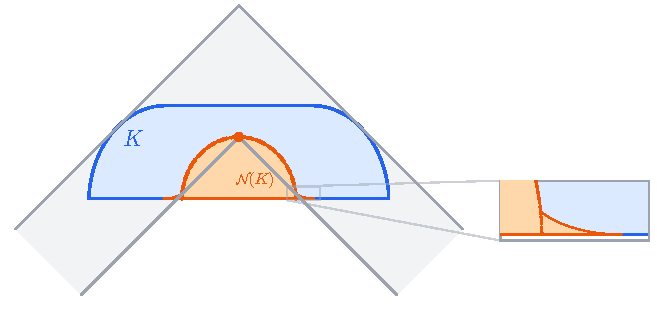
\includegraphics[width=\linewidth]{figures/fig-capniche}
  \caption{Gerver's cap $K$, the union of the blue and the orange regions, and
  its niche $\cN(K)$ (orange); the sofa $\Gs=K\setminus\cN(K)$ is the blue
  region. Grey: the copy of the hallway at the angle $t=\pi/4$. Its outer walls
  touch $K$, and its inner corner (orange dot) lies on the dashed curve, the
  path of the inner corner of the copies as $t$ runs from $0$ to $\pi/2$. Near
  its two ends the niche extends beyond this path, down to the floor, where the
  inner walls, not the corner, touch the sofa; the inset magnifies the right
  end, and the left end is its mirror image.}
  \label{fig:capniche}
\end{figure}

\begin{figure}[htbp]
  \centering
  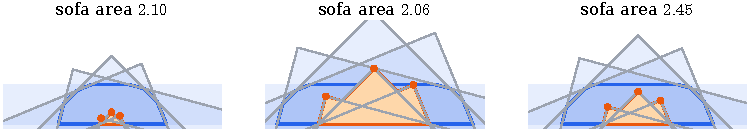
\includegraphics[width=\linewidth]{figures/fig-placements}
  \caption{Three placements of copies of the hallway at the same three angles
  $t=\pi/8,\pi/4,5\pi/12$ (orange dots: their inner corners). Each copy shades
  in light blue the region inside its two outer walls, and so do the start and
  end positions, which keep the sofa in the strip $0\le y\le1$; the polygonal
  cap, outlined in blue, is the darkest region, where all of them overlap, and
  the polygonal niche (orange) is the part of the cap beyond both inner walls of
  at least one copy. Left: copies close in give a small cap. Middle: copies far
  out give a large cap, but also a large niche. Right: a maximum polygon cap for
  these angles.}
  \label{fig:placements}
\end{figure}

\begin{figure}[htbp]
  \centering
  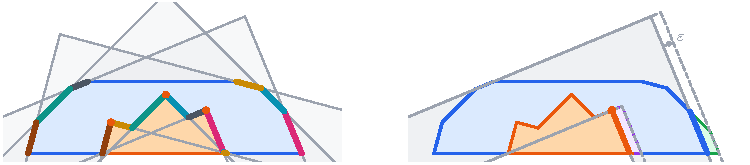
\includegraphics[width=\linewidth]{figures/fig-balance}
  \caption{Balance of the maximum polygon cap of \cref{fig:placements}. Left:
  the three copies of the hallway (light grey; orange dots: their inner
  corners); each slanted side of the cap lies on an outer wall of one of the
  copies, and is drawn thick in the same colour as the side of the niche on the
  inner wall of the same copy parallel to it; the two have the same length. A
  side of the niche may consist of several pieces, as for the amber pair. Right:
  Gerver's balancing argument. The copy at the angle $\pi/8$ (light grey) is
  moved outward by $\eps$ (dashed), which moves one of its outer walls and the
  inner wall parallel to it and leaves the other two walls in place. This adds
  to the cap a strip along its side on that wall (green), and to the niche a
  strip along its side on the inner wall (purple); the two sides are drawn
  thick. The sofa area changes by about $\eps$ times the difference of their
  lengths, so if they differed, moving the walls outward or inward would
  increase it; here the two sides have the same length, $0.63$, as they do at
  each of the six slanted sides of this cap.}
  \label{fig:balance}
\end{figure}

\begin{figure}[htbp]
  \centering
  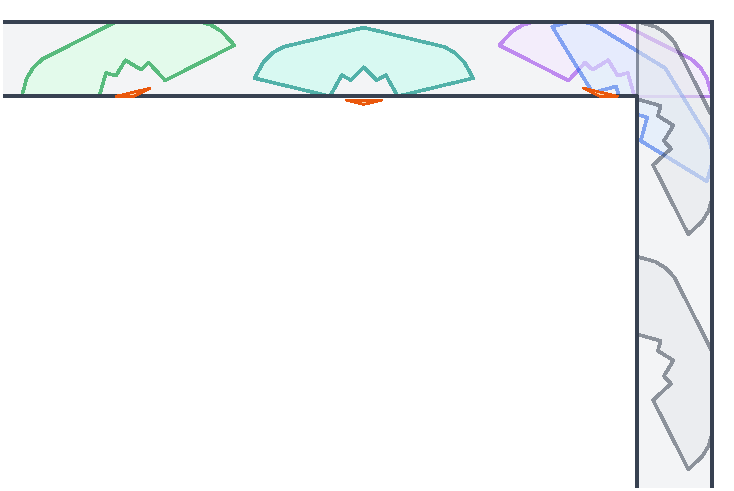
\includegraphics[width=\linewidth]{figures/fig-turn}
  \caption{Step (3a) for an actual sofa: a polygonal cap with rotation angle
  $\omega=1.1$ (about $63^\circ$) minus its niche. A copy of the sofa turned by
  $\pi/2-\omega$ (green) first turns back inside the horizontal side, before the
  corner, through the position halfway (teal), to the sofa's own starting
  position (purple). This is possible because the small triangle at the inner
  corner (orange) lies in the hollow of the sofa, which keeps its height at most
  $1$ throughout this turn. The copy then follows the sofa's own movement and
  turns by $\omega$ around the corner (blue halfway, grey at the end, and again
  slid down the vertical side). In total, it turns by the full right angle.}
  \label{fig:turn}
\end{figure}

\begin{figure}[htbp]
  \centering
  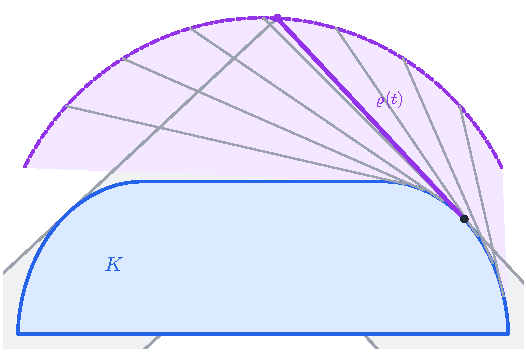
\includegraphics[width=0.75\linewidth]{figures/fig-mamikon}
  \caption{One of the terms of $\cQ$ in step (4), for Gerver's cap $K$. For an
  angle $t$, the segment of length $\varrho(t)$ runs along an outer wall of the
  copy of the hallway at the angle $t$, from the point where $K$ touches that
  wall (black dot) to the outer corner of the copy (purple dot); the copy at the
  angle $t$ is drawn in light grey, with its two outer walls touching $K$. The
  thin grey segments are the same segment for other angles. As $t$ runs from
  $\varphi$ to $\pi/2-\varphi$, where $\varphi=0.039\ldots$ is Gerver's angle
  (Appendix~\ref{app:gerver}) and this is the range of angles in which the inner
  corner of the hallway touches Gerver's sofa, the segment sweeps the shaded
  region, whose area is $\frac12\int\varrho(t)^2\dd t$ by Mamikon's theorem; the
  dashed curve is the path of the outer corner.}
  \label{fig:mamikon}
\end{figure}

\section{Gerver's sofa}\label{app:gerver}

We recall Romik's description of Gerver's sofa~\cite[Section~4]{Romik18}, in the form used by~\cite{Baek} and by the formalization. Let
$t_0=0<t_1=\varphi<t_2=\theta<t_3=\pi/2-\theta<t_4=\pi/2-\varphi<t_5=\pi/2$. A \emph{parameter tuple} consists of the angles $\varphi,\theta$,
numbers $a_1,a_2,b_1,b_2,c_1,c_2,d_1,d_2,e_1,e_2$ and points $\kappa_1,\dots,\kappa_5\in\R^2$ (22 real parameters). The \emph{rotation path} $\xx:[0,\pi/2]\to\R^2$
is $\xx=\xx_i$ on the $i$th phase, where the phases are $[0,t_1)$, $[t_1,t_2)$, $[t_2,t_3]$, $(t_3,t_4]$ and $(t_4,t_5]$, and
\begin{align*}
  \xx_1(t)&=R_t\bigl(a_1\cos t+a_2\sin t-1,\ -a_2\cos t+a_1\sin t-\tfrac12\bigr)+\kappa_1,\\
  \xx_2(t)&=R_t\bigl(-\tfrac{t^2}4+b_1t+b_2,\ \tfrac t2-b_1-1\bigr)+\kappa_2,\\
  \xx_3(t)&=R_t\bigl(c_1-t,\ c_2+t\bigr)+\kappa_3,\\
  \xx_4(t)&=R_t\bigl(-\tfrac t2+d_1-1,\ -\tfrac{t^2}4+d_1t+d_2\bigr)+\kappa_4,\\
  \xx_5(t)&=R_t\bigl(e_1\cos t+e_2\sin t-\tfrac12,\ -e_2\cos t+e_1\sin t-1\bigr)+\kappa_5 .
\end{align*}
The pieces of a solution agree at the ends of the phases, by condition~(3) below, so the conventions at the ends matter only for other tuples.
For a differentiable curve $\xx$ let $\alpha=\ip{\xx'}{u_t}$, $\beta=\ip{\xx'}{v_t}$, and let $\bA,\bB,\bC,\bD$ be as in \cref{sec:gerver}. The tuple \emph{solves Romik's
equations} if $0<\varphi<\theta<\pi/4$ and:
\begin{enumerate}[label=(\arabic*)]
\item (left--right symmetry) $e_1=a_1$, $e_2=-a_2$, $d_1=\frac\pi4-b_1$, $d_2=b_2+\frac\pi4\bigl(2b_1-\frac\pi4\bigr)$, $c_2=c_1-\frac\pi2$;
\item (the start) $\kappa_1=(1-a_1,\frac14)$ and $a_2=-\frac14$, so that $\xx(0)=O$ and $\bA(0)=(1,0)$;
\item (continuous differentiability) $\xx_i(t_i)=\xx_{i+1}(t_i)$ and $\xx_i'(t_i)=\xx_{i+1}'(t_i)$ for $i=1,2,3,4$;
\item (the contact conditions) $\xx_1(t_1)=\bB_4(t_3)$ and $\xx_5(t_4)=\bD_2(t_2)$, where $\bB_4=\xx_4+\alpha_4v_t$ and $\bD_2=\xx_2-\beta_2u_t$ are the contact
curves of $\xx_4$ and $\xx_2$.
\end{enumerate}
These are Romik's equations (27)--(44). \emph{Gerver's sofa} is the shape of the rotation path of the solution with $\varphi\in[0.039,0.04]$ and $\theta\in[0.68,0.69]$, which is
unique in this box (\cref{fact:gerver}\ref{fact:gerver:def}). Its numerical values, to ten decimal places, are
\[
\begin{array}{ll}
  \varphi=0.0391773648, & \theta=0.6813015094,\\
  a_1=e_1=1.2103224221, & a_2=-e_2=-0.25,\\
  b_1=-0.5276245980, & b_2=0.9202583852,\\
  c_1=0.6260455228, & c_2=-0.9447508039,\\
  d_1=1.3130227614, & d_2=-0.5253826704,
\end{array}
\]
\[
\begin{array}{l}
  \kappa_1=(-0.2103224221,\ 0.25),\quad \kappa_5=(-1.0172040368,\ 0.25),\\
  \kappa_2=(-0.9191792928,\ 0.4724066198),\\
  \kappa_3=(-0.6137632294,\ 0.8896264790),\\
  \kappa_4=(-0.3083471661,\ 0.4724066198),
\end{array}
\]
and $\xx(\pi/2)=(-1.2275264589,0)$, $\max_t\xx(t)_y=\xx(\pi/4)_y=0.6642678135$, $\xx(t_1)_y=\xx(t_4)_y=0.0551867605$. The area is $\abs\Gs=2.21953166887\ldots$ (Gerver, Romik), and
$2.2192\le\abs\Gs\le2.2199$ is proved in~\cite{Companion}. In Gerver's own parametrization the constants $A=0.0944265608$ and $B=1.3992037273$ together with $\varphi$ and
$\theta$ solve a system of four equations~\cite{Gerver92}, from which the 22 parameters above are computed.

The contact curves $\bA,\bB,\bC,\bD$ are the points where the sides of the hallway touch the sofa. The sofa touches the walls $a(t)$ and $c(t)$ at $\bA(t)$ and $\bC(t)$
for all $t$; the wall $d(t)$ at $\bD(t)$ for $t\in[t_0,t_2]$; the wall $b(t)$ at $\bB(t)$ for $t\in[t_3,t_5]$; and the inner corner touches it at $\xx(t)$ for
$t\in[t_1,t_4]$. As in~\cite{Gerver92,Romik18}, the boundary of $\Gs$ consists of 18 pieces: $\bA$ on four phases, the top edge, $\bC$ on four phases, an edge on the $x$-axis, $\bD$ on two phases, $\xx$ on three phases,
$\bB$ on two phases, and a second edge on the $x$-axis.

\section{Corrections to the statements of \texorpdfstring{\cite{Baek}}{Baek's paper} that are used here}\label{app:corrections}

The audit that accompanies the formalization compared every result of~\cite{Baek} with its TeX source and with the formal statement~\cite{Companion}. Every result of the paper
holds with the intended statement. \cref{tab:corrections} lists the corrections that concern the results used in this paper, with the labels E$n$ of the audit. The complete list of the audit has
27 items, E22 only pointing to E21, and two missing hypotheses: \baek{Thm.~2.1.1} (Schneider's Theorem~4.2.3: $\sigma_K(X)$ is the length of $\bigcup_{t\in X}e_K(t)$) needs
$K$ to have interior points, and \baek{Thm.~3.1.2} needs a bounded Nef polygon; every use satisfies them (the text itself uses $\sigma_K$ only as defined in \cref{fact:convex}\ref{fact:convex:sigma}, which does not depend on Thm.~2.1.1). Twelve of the findings in the audit come from the notes of the formalization~\cite{Cureton}.

{\small
\begin{longtable}{@{}>{\raggedright\arraybackslash}p{0.065\linewidth}>{\raggedright\arraybackslash}p{0.19\linewidth}>{\raggedright\arraybackslash}p{0.37\linewidth}>{\raggedright\arraybackslash}p{0.22\linewidth}@{}}
\caption{Corrections to~\cite{Baek} that concern the results used here.}\label{tab:corrections}\\
\toprule
Item & Result of~\cite{Baek} & Correction & Where here\\
\midrule\endfirsthead
\toprule
Item & Result of~\cite{Baek} & Correction (continued) & Where here\\
\midrule\endhead
\bottomrule\endlastfoot
E1 & Def.~2.3.9 & the left and right side of a line are defined for lines not parallel to the $x$-axis (printed: $y$-axis) & \cref{fact:monotone}\ref{fact:monotone:envelope}\\
E2 & Thm.~2.4.1, 2.4.2 & the union over $t\in[0,\omega]$ and over $(0,\omega)$ agree, since $F_\omega\cap Q^-_K(0)=F_\omega\cap Q^-_K(\omega)=\emptyset$; $\cC(S)$ is bounded also for $\omega=\pi/2$ & \cref{fact:monotone}\ref{fact:monotone:cap}\\
E3 & Prop.~2.5.4 & the reflection exchanges the walls ($a\leftrightarrow c$, $b\leftrightarrow d$) and the ends $W\leftrightarrow Z$; $K$ and not $K^{\mir}$ stands on the right of the vertex identity & \cref{fact:monotone}\ref{fact:monotone:mirror}, \cref{lem:triangle}, \cref{prop:curvature}\\
E4 & Lemma~2.5.6, Thm.~2.5.8 (and Lemma~3.4.8, Remark~3.4.1) & used without proof, true for every cap: $A_K^-(0)=(h_K(0),0)$, $C_K^+(\omega)=h_K(\omega+\pi/2)v_\omega$, and $O\in K$ if $\omega<\pi/2$; the same holds for $o_\omega$, which Lemma~3.4.8 and Remark~3.4.1 use (not in the audit) & \cref{lem:ends}, \cref{lem:contains}, \cref{lem:wedge}, \cref{lem:sandwich}\\
E5 & Thm.~3.1.2, Lemma~3.4.7 & the Nef polygon must be bounded; the two applications of the theorem for a pinned normal change disjoint strips & \cref{fact:push}\\
E6 & Def.~3.2.5 & $\cN_\Theta(K)=F_\omega\cap\bigcup_{t\in\Theta}Q^-_K(t)$ (printed: $P_\omega$ in place of $F_\omega$); with $P_\omega$, Prop.~3.3.5 and Lemma~3.4.2 are false & \cref{sec:polygon}, \cref{fact:width}, \cref{prop:penmax}\\
E7 & Prop.~3.3.1\,(2) & normal angles in $\Theta^\diamond\cup\{\omega+\pi,3\pi/2\}$ (printed: $\Theta^\diamond$) & \cref{sec:polygon}\\
E8 & Thm.~3.4.3, 3.5.2, 3.5.4 & minor gaps: a Hausdorff limit of polygon caps is a polygon cap (resp.\ a cap), and the niche of the limit lies in the polygon niches eventually, point by point & \cref{prop:penmax}, \cref{prop:selection}, \cref{lem:limsup}\\
E9 & Lemma~4.2.4 & the range is $\omega\in[\sec^{-1}(2.2),\pi/2)$ (printed: $[\tan^{-1}(2.2),\pi/2)$) & \cref{fact:corner}\\
E10 & Thm.~4.2.5, 1.5.2 & the width bound for the pentagon $P_\omega\setminus\Delta_\omega$ is asserted without proof; the proof puts the vertices of $\Delta_\omega$ in the open quarter-plane & \cref{lem:triangle}, \cref{lem:width}\\
E12 & Thm.~6.1.2 & the proof (Gerver's Thm.~2 makes $\Gs$ a balanced maximum sofa) is invalid; the statement is true and follows from Romik's equations & \cref{fact:gerver}\ref{fact:gerver:cap}\\
E13 & Prop.~6.2.2 & $f^\pm_{K^{\mir}}(t)=g^\mp_K(\pi/2-t)$, and likewise for $g$ (printed: without the change of angle) & \cref{fact:arms}\ref{fact:arms:mirror}\\
E14 & Def.~6.2.2, Thm.~6.2.3 & $\partial^+$ is the right derivative (Def.~6.2.2 calls it the left one), and the second display of Thm.~6.2.3 is about $\partial^-\xx_K$ & \cref{fact:arms}\ref{fact:arms:deriv}\\
E15 & Lemma~6.3.1 & cites Thm.~3.5.4 (balanced maximum caps) for $\cN(K)\subset K$ of a maximum polygon cap; the applicable result is Thm.~3.4.10, which gives what the lemma needs, and the lemma holds & not used here (the box of \cref{prop:penmax} bounds the diameter)\\
E17 & Lemma~6.5.2--6.5.5, Thm.~6.5.6 & $f_K(0)=1$ is used without being stated; Lemma~6.5.5 is used on $(0,\pi/2]$ (printed: $(0,1]$) & \cref{fact:arms}\ref{fact:arms:regular}, \cref{fact:iteration}\ref{fact:iteration:eleven}\\
E20 & Lemma~8.3.5 & the arc $\mathbf u_K^{0,\pi}$ is outside the range $b<a+\pi$ of \baek{Thm.~7.3.2}; the area is split at the atom $\pi/2$ instead & \cref{fact:Q}\ref{fact:Q:decomp}\\
E21 & Lemma~8.1.7, Thm.~8.2.4 & $\cN(K)\subset K$ is used but not available on $\Ki$; both statements hold and have proofs that avoid it & \cref{fact:Q}\ref{fact:Q:triple}\\
E23 & Lemma~8.3.6\,(3) & the tangent line parametrization is evaluated at $\pi/2$ (printed: at $\varphi^{\mathrm L}$, where the statement is false) & \cref{fact:Q}\ref{fact:Q:decomp}\\
E24 & Thm.~8.4.1 & stated without proof; true, and proved from Romik's equations by interval arithmetic; part (4) holds with one-sided derivatives at the junctions and the ends of the phases. Not in the audit: part (2), read as a Jordan region, omits the open floor segment of $\cN(\KG)$, and the exact description is the identity in \cref{fact:gerver}\ref{fact:gerver:niche} & \cref{fact:gerver}\\
E25, E26 & Thm.~8.4.3\,(2), Prop.~8.4.4\,(4) & $\bB(t_3)$ (printed: $\bD(t_3)$); the measure $\breve\sigma_D$ lives on $(\pi/2+t_0,\pi/2+t_2]$ with a shifted density & \cref{fact:Q}\ref{fact:Q:max}\\
E27 & several & misprints: the second half-plane of $Q^-_S(t)$ lacks its ``$-1$'' (Prop.~2.2.2); the sign of the change of $\abs{\cN_\Theta}$ in the proof of Lemma~3.4.7; $\cR_B$ starts at $\pi+\varphi^{\mathrm R}$, not $\pi/2+\varphi^{\mathrm R}$ (Def.~8.3.3); the statement of Thm.~2.1.3 & \cref{sec:sofas}, \cref{fact:convex}, \cref{fact:push}, \cref{sec:Q}\\
\end{longtable}
}

\section{The Lean formalization: the statement and a dictionary}\label{app:lean}

\subsection{The statement of \texorpdfstring{\cref{thm:main}}{the main theorem}}

The statement of record is \path{Baek.gerver_sofa_unique} in \texttt{Challenge.lean}. It uses Mathlib's vocabulary and the definitions below, which \texttt{Challenge.lean}
copies verbatim from \texttt{ChallengeDefs.lean}; they are those of this paper. In Lean the plane is $\R\times\R$, the area of a set is its Lebesgue measure \path{volume}, and
\texttt{rot t} is the counterclockwise rotation by $t$.
\begin{itemize}
\item \path{horizSide} $=\{p:\ p_1\le1,\ 0\le p_2\le1\}=H_L$, \path{vertSide} $=\{p:\ 0\le p_1\le1,\ p_2\le1\}=V_L$, \path{hallway} $=H_L\cup V_L=L$.
\item \texttt{IsMovingSofa S} holds if $S$ is closed and connected (hence nonempty) and there are $\theta:\R\to\R$ and $c:\R\to\R^2$, continuous on $[0,1]$, with $\theta(0)=0$,
$\mathrm{rot}_{\theta(0)}p+c(0)\in H_L$ for $p\in S$, $\mathrm{rot}_{\theta(s)}p+c(s)\in L$ for $p\in S$ and $s\in[0,1]$, and $\mathrm{rot}_{\theta(1)}p+c(1)\in V_L$ for $p\in S$ (\cref{def:sofa}, the rotation
angle $-\theta(1)$ being left free).
\item \texttt{shapeOfPath x} $=H_L\cap\bigcap_{t\in[0,\pi/2]}\bigl(\xx(t)+R_tL\bigr)\cap\bigl(\xx(\pi/2)+R_{\pi/2}V_L\bigr)$, written in Lean with images of the hallway sets under $p\mapsto \xx(t)+\mathrm{rot}_t\,p$.
\item \path{GerverParams} holds the 22 parameters of Appendix~\ref{app:gerver}; \texttt{P.path} is the rotation path glued from the five curves of Appendix~\ref{app:gerver}; \texttt{P.IsSolution} is the conjunction of
$0<\varphi<\theta<\pi/4$ and the four groups (1)--(4) of Appendix~\ref{app:gerver} (Romik's equations (27)--(44)); \texttt{P.InBox} says $\varphi\in[0.039,0.04]$, $\theta\in[0.68,0.69]$; and \texttt{gerverSofa P} $=$ \texttt{shapeOfPath P.path}.
\end{itemize}
The theorem: for every \texttt{P : GerverParams} with \texttt{P.IsSolution} and \texttt{P.InBox}, and every set $S\subset\R\times\R$ with \texttt{IsMovingSofa S} and
\texttt{volume S = volume (gerverSofa P)}, there are $\theta\in\R$ and $v\in\R\times\R$ such that the image $\{\mathrm{rot}_\theta p+v:p\in S\}$ equals \texttt{gerverSofa P}. The theorems \path{Baek.gerver_params_exists}
and \path{Baek.gerver_params_unique} say that the box contains exactly one solution, so that \texttt{gerverSofa P} is Gerver's sofa $\Gs$, and \path{Baek.gerver_sofa_area} says that its area
lies between $2.2192$ and $2.2199$.

\subsection{Dictionary}

\cref{tab:dict} lists the declarations that prove the results of this paper. The modules are in the repository~\cite{Companion}: a name followed by a module in parentheses is in
\texttt{MovingSofaUniqueness/} (\texttt{Main}, \texttt{Selection}, \texttt{Variation}, \texttt{AngleExtension}, \texttt{Curvature}, \texttt{Rigidity}, \texttt{RegularClosed}, \texttt{Rigid}) or, with a directory, in
\texttt{MovingSofaOptimality/}. The results of~\cite{Baek} are in \texttt{MovingSofaOptimality/}, under the name \path{theorem}$n_1$\path{_}$n_2$\path{_}$n_3$ (also \path{lemma}, \path{proposition}, \path{corollary}) for the result number $n_1.n_2.n_3$ of~\cite{Baek}.
Some statements are slightly different in Lean: \cref{lem:nichebox} has the box $[-R,R]\times[0,2R]$, \cref{lem:sum} has $2B$ for $B$, \cref{lem:triangle} has the closed quarter-plane in \path{consumed_of_pinned} (the open one is in the
other declarations listed), \cref{lem:cell} is stated with $g_K^-(t+\delta)$, and \cref{fact:sides}\ref{fact:sides:identity} is formalized in its sine form (see \cref{sec:formalization} for the others). The converse part of \cref{thm:caps} (a translate of $\KG$ has sofa area $\abs\Gs$) and
\cref{rem:translate} are not stated in Lean, and \cref{cor:all} only in the vocabulary of formal-conjectures (\path{FormalConjectures.MovingSofa.volume_eq_sofaConstant_iff_congruent_gerversSofa}).

{\footnotesize
\begin{longtable}{@{}>{\raggedright\arraybackslash}p{0.21\linewidth}>{\raggedright\arraybackslash}p{0.70\linewidth}@{}}
\caption{The results of this paper and the Lean declarations that prove them.}\label{tab:dict}\\
\toprule Result & Lean declarations\\ \midrule\endfirsthead
\toprule Result & Lean declarations (continued)\\ \midrule\endhead
\bottomrule\endlastfoot
\cref{thm:main} & \path{Baek.gerver_sofa_unique} (\texttt{Challenge.lean}); \path{MovingSofaUniqueness.image_eq_gerver_of_volume_eq}, \path{maximizer_contained_in_gerver} (\texttt{Main})\\
\cref{prop:reduction} & \path{maximal_envelope}, \path{own_cap_isMax}, \path{isMaxCap_of_area_eq}, \path{cap_area_le_gerver} (\texttt{Main}); \cref{fact:optimal}: \path{theorem1_1_1}, \path{theorem3_5_5}, \path{theorem3_5_6}\\
\cref{lem:recovery}, \cref{lem:box}, \cref{lem:nichebox} & \path{SupportSamples.penalty_recovery_zero}, \path{dyadic_recovery_ge}, \path{polygon_subset_sampleBox}, \path{niche_subset_box}, \path{polyNiche_subset_box} (\texttt{Selection})\\
\cref{prop:penmax} & \path{exists_penalizedMax}, \path{exists_dyadic_penalizedMax}, \path{selected_objective_ge}, \path{selected_sequence_bounded} (\texttt{Selection})\\
\cref{lem:limsup}, \cref{lem:dyadic}, \cref{prop:selection} & \path{dyadic_objective_limsup}, \path{caps_eq_of_dyadic_supports}, \path{exists_selectedCapSequence}, \path{penalty_tendsto_zero_of_objective} (\texttt{Selection})\\
\cref{lem:floating}, \cref{prop:floating} & \path{floatingCap}, \path{floatingCap_polygon}, \path{subset_floatingCap}, \path{floatingCap_support_bounds}, \path{floatingCap_support_other}, \path{floating_penalty_growth}, \path{floating_defect_le} (\texttt{Variation})\\
\cref{lem:sandwich}, \cref{lem:back}, \cref{prop:pinned} & \path{pinned_contract_mem}, \path{pinned_div_mem}, \path{pinned_raw_support_bound}, \path{translated_strip_support}, \path{pinned_translation_bound}, \path{pinned_normalized_support_bound}, \path{pinned_defect_le} (\texttt{Variation})\\
\cref{cor:twosided} & \path{polygon_weighted_defect_zero}, \path{abs_selected_defect_le}, \path{selectorDefectBound} (\texttt{Variation})\\
\cref{lem:wedge}, \cref{lem:cont}, \cref{lem:usc}, \cref{prop:pinned-bounds} & \path{ang_wedgeGapWInf_le_tau}, \path{ang_wedgeGapZInf_le_tau}, \path{lemma4_1_1}, \path{ang_abs_wedgeGapZInf_sub_le}, \path{ang_le_sigmaAt_of_tendsto} (\texttt{Angle/HorizontalSide}); \path{pinned_bounds_of_maximal_positive} (\texttt{Variation})\\
\cref{lem:triangle}, \cref{fact:corner}, \cref{lem:width}, \cref{lem:turn}, \cref{prop:U} & \path{consumed_of_pinned}, \path{right_angle_motion_of_pinned_bounds} (\texttt{AngleExtension}); \path{lemma4_2_2}, \path{lemma4_2_4}, \path{theorem4_2_5}, \path{ang_three_points_mem}, \path{ang_consumed_of_supp_zero}, \path{ang_mirror_mem_qMinus}, \path{ang_mem_niche_of_small}, \path{ang_width_le_one}, \path{right_angle_motion_of_width} (\texttt{Angle/RightAngle}); \path{maximal_monotone_has_right_angle} (\texttt{Main})\\
\cref{lem:wall}, \cref{lem:tau}, \cref{lem:curv-defect} & \path{polygon_tau_le_geom}, \path{polygon_curvature_with_defect} (\texttt{Curvature}); \path{inj_param_minus}, \path{inj_param_plus}, \path{inj_polygon_sigmaAt_eq}, \path{inj_not_mem_qMinus} (\texttt{Injectivity/DiscreteIneq})\\
\cref{lem:cell}, \cref{lem:sum} & \path{polygon_arm_cell}, \path{polygon_step_with_error}, \path{polygon_Ico_with_errors}, \path{polygon_Ioo_with_errors} (\texttt{Curvature})\\
\cref{lem:lsc}, \cref{lem:limit} & \path{curvature_Ioo_limit}, \path{firstCurvature_of_Ioo}, \path{firstCurvature_of_polygon_errors} (\texttt{Curvature})\\
\cref{prop:curvature} & \path{sampled_grid_error_le}, \path{diameter_le_box}, \path{firstCurvature_of_maximal_positive}, \path{secondCurvature_of_mirror_first}, \path{curvature_of_maximal_positive} (\texttt{Curvature})\\
\cref{lem:integral}, \cref{lem:lower}, \cref{prop:inj}, \cref{cor:Ki} & \path{injCond1_of_curvature}, \path{first_arm_integral_lower}, \path{second_arm_integral_lower}, \path{lowerSeq_le_of_integral_bounds}, \path{arms_strict_of_curvature}, \path{injectivity_of_curvature} (\texttt{Curvature}); \path{isKi_of_maximal_area} (\texttt{Main})\\
\cref{lem:equality}, \cref{lem:tangent} & \path{ki_maximizer_equality_conditions}, \path{halfSquareIntegral_combo_gap}, \path{displacement_eqOn_of_mamikon_eq}, \path{tangentKernel_of_mamikon_eq}, \path{middleKernel_of_mamikon_eq} (\texttt{Rigidity})\\
\cref{prop:kernel}, \cref{lem:translate}, \cref{thm:caps} & \path{capKernel_of_mamikonS_eq}, \path{capKernel_of_triple_midpoint}, \path{CapKernel.eq_horizontal_translation}, \path{mem_cap_sub_horizontal_iff}, \path{sofa_eq_translate_of_upper_support} (\texttt{Rigidity}); \path{ki_sofa_eq_gerver_translate}, \path{right_angle_monotone_eq_gerver} (\texttt{Main})\\
\cref{lem:recover}, \cref{lem:envelope}, \cref{prop:regular} & \path{eq_of_subset_of_measure_eq}, \path{Rigid.recover}, \path{Rigid.volume_image}, \path{Rigid.isClosed_image} (\texttt{Rigid}); \path{regularClosed_cap_sdiff_envelope}, \path{isCompact_envUnder}, \path{envelope_bounds_of_path_height}, \path{envelope_endpoint_order}, \path{gerver_regularClosed} (\texttt{RegularClosed})\\
\cref{fact:height} & \path{GerverParams.path_snd_lt_one} (\texttt{RegularClosed}); \path{gb_x_pos} (\texttt{Gerver/NicheBounds})\\
\midrule
\cref{fact:convex} & \path{proposition2_1_2}, \path{theorem5_2_2}, \path{sigma_Ioc}, \path{sigma_periodic} (\texttt{Basic/SurfaceArea})\\
\cref{fact:angle}, \cref{fact:monotone}, \cref{lem:contains}, \cref{lem:ends} & \path{theorem1_5_1}; \path{proposition2_3_1_exists}, \path{proposition2_3_1_subset}, \path{theorem2_3_2}, \path{lemma2_3_5_supp}, \path{theorem2_4_1}, \path{theorem2_4_2}, \path{theorem2_4_3}, \path{theorem2_5_9}, \path{theorem2_5_10}, \path{proposition2_5_4_isCap}, \path{proposition2_5_4_supp}, \path{proposition2_5_4_hallway}, \path{proposition2_5_4_sets}, \path{proposition2_5_4_sigma}, \path{sofaArea_mirror} (\texttt{Curvature}); \path{IsCap.zero_mem}, \path{IsCap.oPt_mem} (for \cref{lem:contains}); \path{IsCap.cPlus_eq_corner}, \path{IsCap.aMinus_eq_corner} (for \cref{lem:ends})\\
\cref{fact:polygon}, \cref{fact:width}, \cref{fact:sides}, \cref{fact:push} & \path{proposition3_2_1}, \path{proposition3_2_2}, \path{theorem3_2_3}; \path{lemma3_4_2}; \path{lemma3_4_5_one}, \path{lemma3_4_5_two}, \path{mpc_walk_total}, \path{mpc_sum_sigma_sin}, \path{mpc_sum_tau_sin}; \path{lemma3_4_7}, \path{lemma3_4_8}, \path{proposition3_3_7}, \path{theorem3_3_6}, \path{theorem3_1_2}\\
\cref{fact:arms}, \cref{fact:iteration} & \path{theorem6_2_3_right}, \path{theorem6_2_3_left}, \path{theorem6_2_5}, \path{proposition6_2_2}, \path{proposition6_4_5}, \path{proposition6_4_6_deriv}, \path{proposition6_4_6_continuous}; \path{lemma6_4_2}, \path{lemma6_5_5}\\
\cref{fact:Q} & \path{theorem8_1_8}, \path{theorem8_2_4}, \path{lemma8_3_3}, \path{lemma8_3_4}, \path{lemma8_3_7}, \path{theorem8_3_1}, \path{theorem8_3_2}, \path{theorem8_3_8}, \path{corollary8_5_8}, \path{theorem8_4_6}, \path{theorem7_1_2_sigma}, \path{theorem7_1_2_supp}, \path{theorem7_1_2_vertices}, \path{theorem7_4_1}, \path{theorem7_4_2}\\
\cref{fact:gerver} & \path{definition8_1_2_exists}, \path{definition8_1_2_unique}, \path{Baek.gerver_sofa_area}, \path{gerverSofa_area_mem}, \path{theorem8_4_1_monotone}, \path{theorem8_4_1_walls}, \path{theorem8_4_1_tangents}, \path{theorem8_4_1_niche} (the boundary curves and the area), \path{gn_niche_eq}, \path{env_niche_eq} (the exact description of the niche), the strict monotonicity lemmas for the abscissa along $\bD$, $\xx$ and $\bB$ (\texttt{Gerver/Envelope}), \path{theorem6_1_2}
\end{longtable}
}

\section{The use of AI}\label{app:ai}

ChatGPT Pro~6 (OpenAI) wrote the first version of the proof of \cref{thm:main}
on 2 October 2026, at the author's request, together with drafts of its
formalization and of the connection with formal-conjectures; neither Lean draft
had ever been compiled. Claude Opus~5.5 (Anthropic), in Claude Code with
sub-agents, formalized~\cite{Baek} and completed the two drafts, following the
author's \texttt{formalize-math-paper} procedure, in rounds between 1 and 3
October 2026; 54 proofs of the first draft and 78 proofs of the second did not
compile and were replaced and proved again. Before any proof was written, a
separate run of Claude Opus~5.5 reviewed every Lean statement of a result
of~\cite{Baek} against its TeX source, and a later separate run compared the
Lean statements of uniqueness with the informal proof and found no weakening,
vacuous definition or hidden assumption. The repository~\cite{Companion} records
who did what, with times and sizes. Claude Sonnet~5.5 (Anthropic), in Claude
Code, wrote the first version of this manuscript on 4 October 2026 from the Lean
library, the illustrated text of the proofs in~\cite{Companion} and the text
of~\cite{Baek}. All figures but one were computed from the definitions by the
script \path{docs/paper/figures/make_figures.py} of the
repository~\cite{Companion}; the remaining one is drawn in TikZ. The author
asked for each of these steps and decided its scope. None of the three systems
is an author of this paper, since none of them can take responsibility for it.
The author has proofread and edited the abstract and \cref{sec:intro}, and has
not yet read the other sections; they have been checked only by the runs
described below.

The text of this paper is not machine-checked; the dictionary of
Appendix~\ref{app:lean} gives its correspondence with the Lean statements. On 4
October 2026, six runs of Claude Opus~5.5, each assigned some sections, compared
the statements and proofs of the first version of this paper with the Lean
statements and with the TeX source of~\cite{Baek}; a run of Claude Sonnet~5.5
checked the claims about the formalization, the dictionary and the references;
and a run of Claude Opus~5.5 read the whole paper without access to either. The
findings were corrected, and a further run of Claude Opus~5.5 checked the
passages rewritten in response. Two more runs of Claude Opus~5.5 checked a
rewrite of the prose for the patterns of machine-written text and for changes of
claim. The same day, the Lean library was extended with the results of this
paper that it did not yet prove, and Sections~2 and 4 to 9 were rewritten, by
sub-agents running Claude Opus~5.5, to state what the Lean states and to follow
its proofs. Five runs of Claude Opus~5.5, each assigned some sections and
appendices, then compared the result with the Lean, and a second round of the
same runs compared the corrected text again. The changes that followed the
second round were not checked again.

On 5 October 2026, ChatGPT Pro~6 wrote the second proof of optimality
(\cref{rem:second}) in Lean, with a plan for presenting it in this paper. The
Lean code had never been compiled. It came as a pull request to the repository,
which Claude Opus~5.5, in Claude Code, merged at the author's request. The code
compiled without change and passed the audit that came with it, and also an
extended audit, written by Claude Opus~5.5, that covers the results from which
Baek derives step~(3) of \cref{sec:baek}. From the Lean, Claude Opus~5.5 then
wrote a subsection on this proof, \cref{fact:exists} and the passages that refer
to them in Sections~\ref{sec:intro} to~\ref{sec:reduction}
and~\ref{sec:formalization} and Appendices~C and~D. Two more runs of Claude
Opus~5.5 checked these passages, one against the Lean and one for their prose,
and their findings were applied. At the author's request, Claude Opus~5.5 also
wrote the sentence of the abstract on the second proof. On 6 October, at the
author's request, the subsection was shortened to \cref{lem:right-motion}, at
the end of \cref{sec:right-angle}, and \cref{rem:second}, at the end of
\cref{sec:equality}; \cref{sec:unified} gives the proof in full, with the
certificate.

The same day, ChatGPT Pro~6 wrote the proofs of \cref{sec:stability} as notes
and as Lean code in 85 modules, which had never been compiled; they came as
another pull request. Claude Opus~5.5, in Claude Code with sixteen sub-agents,
made the code compile and merged it, at the author's request. Of its proofs, 123
did not compile and were proved again along the draft's arguments. Twenty lemmas
had lost hypotheses that the draft declared as section variables, since Lean
omits a section variable from a statement that does not mention it; these
hypotheses were added back. A separate run of Claude Opus~5.5 compared every
repaired proof with the draft's and found no change of argument. On 6 October
2026, Claude Opus~5.5 stated the three theorems of stability in
\texttt{Challenge.lean}, and a sub-agent running Claude Opus~5.5 wrote
\cref{sec:stability} and its rows of \cref{tab:dict} from the Lean. The same
session also wrote the sentence of the abstract and the passages of
Sections~\ref{sec:intro} and~\ref{sec:formalization} and
Appendix~\ref{app:lean} on stability, and corrected a sign in the description
of $\cM_K$ in \cref{sec:setting}. Three runs of Claude Opus~5.5 compared the
statements and proofs of \cref{sec:stability} with the Lean, part by part; a
further run compared the new text with the Lean and the repository, and another
read it for its prose. Their findings were applied.

On the evening of 5 October 2026, ChatGPT Pro~6 also wrote a third pull request,
without compiling or running any of it. It contained the library
\texttt{MovingSofaExtremal}, which derives optimality and uniqueness from the
estimates of \cref{sec:stab-certificate,sec:stab-cap}; the module
\texttt{MamikonFoundation} of the stability library, which proves again results
of the module \texttt{Rigidity} of the first proof on square integrals, Mamikon
displacements and the canonical triple; a second solution of twelve statements
of the Challenge
(\texttt{SolutionCoercive.lean}); and the audit
\path{scripts/AuditCoerciveRoute.lean}. It also switched the module
\texttt{MamikonEnergy} of the stability library from importing
\texttt{Rigidity} to importing \texttt{MamikonFoundation}. On 6 October, at the
author's request, Claude Opus~5.5, in Claude Code, merged the manuscript's
branch, which held the compiled stability library, into the pull request's and
compiled the result. One proof did not compile: a \texttt{change} step in the
module \texttt{HorizontalTranslation} whose two sides were not definitionally
equal, which was replaced by a rewrite; one linter warning was also cleared.
The same session then did what the pull request had left for later. It stated
the certificate as one theorem (\cref{thm:certificate}), added to
\texttt{MovingSofaExtremal} the theorem that no rotation is needed
(\cref{thm:unified-uniqueness}\ref{thm:unified-uniqueness:translate}), and
moved two lemmas of that proof, which \cref{cor:translate} shares, from the
module \texttt{Main} to the module \texttt{Rigid}. The stability library had
used the module \texttt{Main} at four places: Baek's theorem twice, for the sign
of the deficit and in the compactness step; the first proof of uniqueness once,
to identify the limit of the compactness step and the normalized sofa of zero
deficit; and the lemma that a moving sofa lies in a horizontal strip of height
one. The session switched these to \texttt{MovingSofaExtremal} and to the moved
lemmas, and made the local cap estimate of the stability library use the
certificate. It then stated \cref{thm:unified}, extended
\texttt{SolutionCoercive.lean} to the fifteen statements of the Challenge, and
rewrote and ran the audit. The pull request was merged the same day. A
sub-agent running Claude Opus~5.5 wrote \cref{sec:unified}, and the passages
that refer to it in the other sections and in Appendices~D and~E, from the
Lean; the session wrote the sentence of the abstract on the single estimate.
Three runs of Claude Opus~5.5, launched by the sub-agent, compared the new
text with the Lean and the repository, part by part, and a fourth checked the
passages rewritten after their reports. Two more runs of Claude Opus~5.5,
neither able to edit, then read the new text, one against the Lean and the
repository and one for its prose. The findings of all these runs were applied;
the edits that followed the last two runs were not checked again. No person has
read \cref{sec:unified}. At the time of writing, the argument of this paper has
not been refereed.


% Appendix F. Reuse the original proof text rather than duplicating or losing it.
% Its original labels remain unique; the main-text restatements use new labels.
\section{Stability}\label{sec:stability}

This section proves that a moving sofa whose area is close to $\abs\Gs$ is,
after a translation, close to $\Gs$, at the rate of the square root of the
missing area, and that this rate is optimal. As in \cref{sec:equality},
$\varphi$ is Gerver's angle, $\KG$ is Gerver's cap and $\cA=\cA_{\pi/2}$. The
\emph{deficit} of a set $S$ of finite area is $\eps(S)=\abs\Gs-\abs S$, which
is nonnegative for moving sofas (\cref{fact:optimal}). Two sets
$X,Y\subset\R^2$ are \emph{$r$-close} if every point of each lies within
Euclidean distance $r$ of a point of the other; for nonempty compact sets, this
means that their Hausdorff distance is at most $r$. For a nonempty compact set
$S$, let $h_S(t)=\max_{p\in S}\ip p{u_t}$. The \emph{normalized} translate
$S^\natural=S+(h_S(\pi)-h_\Gs(\pi),1-h_S(\pi/2))$ has
$h_{S^\natural}(\pi/2)=1$ and $h_{S^\natural}(\pi)=h_\Gs(\pi)$, and $S$ is
\emph{normalized} if $S^\natural=S$. Let $X\triangle Y=(X\setminus
Y)\cup(Y\setminus X)$ be the symmetric difference.

\begin{theorem}[stability of Gerver's sofa]\label{thm:stability}
There are $C,C',\eps_0>0$ such that for every moving sofa $S$ with
$\eps=\eps(S)<\eps_0$, the sets $S^\natural$ and $\Gs$ are
$C\sqrt\eps$-close, and $\abs{S^\natural\triangle\Gs}\le C'\sqrt\eps$.
\end{theorem}

\begin{theorem}[the rotation angle]\label{thm:stability-angle}
There are $C'',\eps_0>0$ such that every moving sofa $S$ with rotation angle
$\omega\in[\omega_0,\pi/2]$ and $\eps(S)<\eps_0$ satisfies
$0\le\pi/2-\omega\le C''\eps(S)$.
\end{theorem}

A \emph{rigid motion} is a map $g(p)=R_\vartheta p+v$. For nonempty compact
sets $X,Y$, $d_{\mathrm{rig}}(X,Y)$ is the infimum of the $d\ge0$ for which
$X$ and $g(Y)$ are $d$-close for some rigid motion $g$. Let $\mathbb B(p,r)$
and $\mathbb B^\circ(p,r)$ be the closed and the open disk of radius $r$ about
$p$.

\begin{theorem}[the exponent $1/2$ is optimal]\label{thm:stability-exponent}
\begin{enumerate}[label=(\alph*)]
\item\label{thm:stability-exponent:family} There are a point $p$ and $r_0>0$
such that for every $r\in(0,r_0)$ the set $\Gs_r=\Gs\setminus\mathbb
B^\circ(p,r)$ is a moving sofa with $\eps(\Gs_r)=\pi r^2$ and
$d_{\mathrm{rig}}(\Gs_r,\Gs)=r$. Moreover, $\Gs_r$ and $\Gs$ are $r$-close,
and $r\le d$ whenever $\Gs_r$ and $g(\Gs)$ are $d$-close for a rigid motion
$g$.
\item\label{thm:stability-exponent:no} Let $a>1/2$, $C\in\R$ and $\eps_0>0$.
There is a moving sofa $S$ with $0<\eps(S)<\eps_0$ such that $S$ and $g(\Gs)$
are $C\eps(S)^a$-close for no rigid motion $g$.
\item\label{thm:stability-exponent:rig} For the same $a$, $C$ and $\eps_0$,
there is a moving sofa $S'$ with $0<\eps(S')<\eps_0$ and
$C\eps(S')^a<d_{\mathrm{rig}}(S',\Gs)$.
\end{enumerate}
\end{theorem}

Baek's functional $\cQ$ is given by a formula \baek{Def.~8.2.2}: for convex
bodies $K$, $B$ and $D$,
\begin{multline}\label{eq:stab-Q}
  \cQ(K,B,D)=\abs K
  +\tfrac12\int_{(3\pi/2,\,3\pi/2+\varphi^{\mathrm L})}h_D\dd\sigma_D
  +\mathcal J\bigl([Y_D,\xx_K(\varphi^{\mathrm L})]\bigr)\\
  -\mathcal J\bigl(\xx_K|_{[\varphi^{\mathrm R},\varphi^{\mathrm L}]}\bigr)
  +\mathcal J\bigl([\xx_K(\varphi^{\mathrm R}),X_B]\bigr)
  +\tfrac12\int_{(\pi+\varphi^{\mathrm R},\,3\pi/2)}h_B\dd\sigma_B ,
\end{multline}
where $X_B=v_B^+(\pi+\varphi^{\mathrm R})$,
$Y_D=v_D^-(3\pi/2+\varphi^{\mathrm L})$ and $\mathcal J([p,q])=\frac12\,p\times
q$; the integrals are the curve areas of two arcs of the boundaries of $D$ and
$B$ \baek{Thm.~7.3.2}. Let $\bar\cT$ be defined as $\cT$ (\cref{sec:Q}), with
$K\in\Kc_{\pi/2}$ in place of $K\in\Ki$; by \cref{lem:stab-variation} below,
$\cQ\le\abs\Gs$ on $\bar\cT$. For $K\in\Kc_{\pi/2}$ let
$s_K=h_{\KG}(\pi)-h_K(\pi)$, so that $K$ and $\KG+(s_K,0)$ have the same
leftmost abscissa.

\begin{theorem}[the cap estimate]\label{thm:stability-cap}
\begin{enumerate}[label=(\alph*)]
\item\label{thm:stability-cap:wide} For every $\xi=(K,B,D)\in\bar\cT$, the
caps $K$ and $\KG+(s_K,0)$ are $2\sec\varphi\sqrt{\abs\Gs-\cQ(\xi)}$-close.
\item\label{thm:stability-cap:ki} For every $K\in\Ki$, the caps $K$ and
$\KG+(s_K,0)$ are $2\sec\varphi\sqrt{\abs\Gs-\cA(K)}$-close.
\item\label{thm:stability-cap:num} $2\sec\varphi\le2500/1249<1001/500$, so
\ref{thm:stability-cap:wide} and \ref{thm:stability-cap:ki} hold with
$1001/500$ in place of $2\sec\varphi$.
\end{enumerate}
\end{theorem}

\Cref{sec:stab-certificate,sec:stab-cap} bound, for every
$\xi=(K,B,D)\in\bar\cT$, the distance from $K$ to $\KG+(s_K,0)$ by a multiple
of $\sqrt{\abs\Gs-\cQ(\xi)}$: with the constant $80$ in
\cref{prop:stab-coercive}, which the proofs of
\cref{thm:stability,thm:stability-angle} use, and with $2\sec\varphi$ in
\cref{thm:stability-cap}. Near $\KG$, Baek's bound $\cA(K)\le\cQ(\xi_K)$ holds
without the injectivity condition (\cref{sec:stab-local}), and a rotation
angle $\omega<\pi/2$ costs area proportional to $\pi/2-\omega$
(\cref{sec:stab-angle}). \Cref{sec:stab-recovery} passes from the cap back to
the sofa, and a compactness argument brings the normalized translate of every
moving sofa of small deficit near $\Gs$ (\cref{sec:stab-entry}); this proves
\cref{thm:stability,thm:stability-angle}. \Cref{sec:stab-puncture} removes
small disks from $\Gs$ to prove \cref{thm:stability-exponent}.

\subsection{The deficit of \texorpdfstring{$\cQ$}{Q} on
\texorpdfstring{$\bar\cT$}{the enlarged domain}}\label{sec:stab-certificate}

Let $\mathcal D$ be a set closed under the Minkowski combinations $c_\lambda$
(\cref{sec:Q}). A functional $\Psi$ on $\mathcal D$ is \emph{quadratic} if
$\Psi(x)=\beta(x,x)$ with $\beta$ convex-linear in each argument; its
\emph{directional derivative} $D\Psi(x;y)$ is the right derivative of
$\lambda\mapsto\Psi(c_\lambda(x,y))$ at $0$ \baek{Def.~7.1.4, Def.~7.1.5}.
Baek shows that $D\Psi(x;y)=\beta(x,y)+\beta(y,x)-2\beta(x,x)$, and that a
quadratic concave $\Psi$ is largest at $x$ if and only if $D\Psi(x;y)\le0$ for
all $y$ \baek{Lemma~7.1.4, Thm.~7.1.5}. Let
$E_\Psi(x,y)=4\Psi(c_{1/2}(x,y))-2\Psi(x)-2\Psi(y)$. As $\beta$ is
convex-linear in each argument,
$E_\Psi(x,y)=\beta(x,y)+\beta(y,x)-\beta(x,x)-\beta(y,y)$, and Baek's formula
for $D\Psi$ gives
\begin{equation}\label{eq:stab-segment}
  \Psi(x)-\Psi(y)=-D\Psi(x;y)+E_\Psi(x,y).
\end{equation}
For a convex body $K$ and a curve $\mathbf z$ as in \cref{sec:Q}, we call
$\varrho_{K,\mathbf z}$ the \emph{displacement} of $\mathbf z$. For convex
bodies $K_0,K_1$, the \emph{energy} $E_\cS(K_0,K_1)$ is the sum, over the four
terms $\cM_K(a,b;\mathbf z_K)$ of $\cS_K$, of
$\frac12\int_a^b(\varrho_{K_0,\mathbf z_{K_0}}-\varrho_{K_1,\mathbf
z_{K_1}})^2\dd t$, and the energies $E_\cR(B_0,B_1)$ and $E_\cL(D_0,D_1)$ are
defined likewise. As the curves of these terms are convex-linear in the body
(\cref{fact:Q}\ref{fact:Q:decomp}), \eqref{eq:gap} gives, for all convex bodies
and $\lambda\in[0,1]$,
\begin{equation}\label{eq:stab-gap}
  (1-\lambda)\cS_{K_0}+\lambda\cS_{K_1}-\cS_{(1-\lambda)K_0+\lambda K_1}
    =\lambda(1-\lambda)E_\cS(K_0,K_1),
\end{equation}
and likewise for $\cR$ and $\cL$, which are therefore convex. Let
$I=[\varphi,\pi/2-\varphi]$.

\begin{lemma}[$\cQ$ on $\bar\cT$]\label{lem:stab-wide}
$\bar\cT$ is closed under Minkowski combinations. On $\bar\cT$,
$\cQ(K,B,D)=\Lambda(K)-\cS_K-\cR_B-\cL_D$, where $\Lambda$, Baek's
$\cP_K+\cS_K$ (\cref{fact:Q}\ref{fact:Q:decomp}), is convex-linear on
$\Kc_{\pi/2}$, and $\cQ$ is quadratic and concave.
\end{lemma}

\begin{proof}
Support functions of Minkowski combinations are the same combinations of the
support functions, so $\bar\cT$ is closed under them. Baek's proof of the
decomposition in \cref{fact:Q}\ref{fact:Q:decomp} \baek{Lemma~8.3.4} uses only
the equalities at the ends of the intervals, so it holds on $\bar\cT$. On
$\Kc_{\pi/2}$, $\abs K$ is the sum of the curve areas of the four arcs of
$\cS_K$ and of the areas $\frac12\sigma_K(t)h_K(t)$ of the triangles spanned by
$O$ and the edges $e_K(t)$, $t=0,\varphi,\pi/2-\varphi,\pi/2,\pi$. Each edge
lies on the supporting line that carries the adjacent end segments
$[v_K^+(a),\mathbf z(a)]$ and $[\mathbf z(b),v_K^-(b)]$ of the Mamikon terms.
In $\cS_K+\cP_K$ \baek{Def.~8.3.4}, the curve areas of the arcs cancel against
$\abs K$, and what remains are $\mathcal J(\yy_K|_I)$, $-\mathcal J(\xx_K|_I)$,
the triangles of the edges and curve areas of segments on the five lines
$l_K(t)$, $t=0,\varphi,\pi/2-\varphi,\pi/2,\pi$. Joining the collinear pieces
on each of these lines gives, with $W_K$ and $Z_K$ as in
\cref{sec:pinned-bounds},
\begin{multline*}
  \Lambda(K)=h_K(0)+h_K(\pi)
  +\frac{2\sin\varphi-h_K(\varphi)-h_K(\pi-\varphi)}{2\cos\varphi}\\
  +\mathcal J(\yy_K|_I)-\mathcal J(\xx_K|_I)+\varsigma_K ,
\end{multline*}
where
\begin{multline*}
  \varsigma_K=\mathcal J([\mathbf l^{\pi/2}_K(\varphi),\yy_K(\varphi)])
    -\mathcal J([W_K(\varphi),\xx_K(\varphi)])\\
  -\mathcal J([\mathbf l^{\pi-\varphi}_K(\pi/2),\yy_K(\pi/2-\varphi)])
    +\mathcal J([Z_K(\pi/2-\varphi),\xx_K(\pi/2-\varphi)]).
\end{multline*}
The differences $\yy_K-\xx_K=u_t+v_t$,
$\mathbf l^{\pi/2}_K(\varphi)-W_K(\varphi)=((1-\sin\varphi)/\cos\varphi,1)$
and
$\mathbf l^{\pi-\varphi}_K(\pi/2)-Z_K(\pi/2-\varphi)
=(-(1-\sin\varphi)/\cos\varphi,1)$ do not depend on $K$, so $\Lambda$ is
convex-linear \baek{Lemma~7.1.6}. The terms of \eqref{eq:stab-Q} are quadratic
\baek{Thm.~7.1.3, Thm.~7.3.2, Thm.~7.1.2, Prop.~7.2.2}, so $\cQ$ is quadratic;
as $\Lambda$ is convex-linear and $\cS,\cR,\cL$ are convex by
\eqref{eq:stab-gap}, $\cQ=\Lambda-\cS-\cR-\cL$ is concave.
\end{proof}

\begin{lemma}[the directional derivative at Gerver's
triple]\label{lem:stab-variation}
For every $\xi\in\bar\cT$, $D\cQ(\xi_G;\xi)\le0$. Hence
$\cQ\le\cQ(\xi_G)=\abs\Gs$ on $\bar\cT$.
\end{lemma}

\begin{proof}
Let $\xi_G=(K_0,B_0,D_0)$ and $\xi=(K,B,D)$, let $\breve\sigma_X$ be the image
of $\sigma_X$ under $t\mapsto t-\pi$, and let $\Delta=h_K-h_{K_0}$,
$\Delta_B(t)=h_B(t+\pi)-h_{B_0}(t+\pi)$ and
$\Delta_D(t)=h_D(t+\pi)-h_{D_0}(t+\pi)$. Baek computes $D\cQ(\xi_G;\xi)$ for
$\xi\in\cT$ \baek{Thm.~8.5.6, Thm.~8.5.7}, using $X_{B_0}=\xx_{K_0}(\varphi)$
and $Y_{D_0}=\xx_{K_0}(\varphi^{\mathrm L})$ \baek{Thm.~8.4.3}. The computation
differentiates only the curves of $\xi_G$, so it holds on $\bar\cT$, and it
gives
\begin{multline*}
  D\cQ(\xi_G;\xi)=\int_{[0,\pi]}\Delta\dd\sigma_{K_0}
  -\int_{I\cup(I+\pi/2)}\Delta\,i_{K_0}\dd t\\
  +\int_{(\varphi,\pi/2)}\Delta_B\dd\breve\sigma_{B_0}
  +\int_{(\pi/2,\pi-\varphi)}\Delta_D\dd\breve\sigma_{D_0}.
\end{multline*}
The four terms are the directional derivatives of $\abs K$, of $-\mathcal
J(\xx_K|_I)$, which is an integral of $\Delta$ against a density $i_{K_0}$, of
the terms of \eqref{eq:stab-Q} that involve $B$ and of those that involve $D$
\baek{Thm.~8.5.2, Thm.~8.5.3}. The first holds for all caps, as $\Delta$
vanishes at $3\pi/2$, the only angle in $(\pi,2\pi)$ that carries
$\sigma_{K_0}$.

Baek shows that, on $[0,\pi]$, $\sigma_{K_0}$ is the sum of the measure with
density $i_{K_0}$ on $I\cup(I+\pi/2)$, of $\breve\sigma_{B_0}$ on
$[\pi/2-\theta,\pi/2)$, of $\breve\sigma_{D_0}$ on $(\pi/2,\pi/2+\theta]$ and of
the atom at $\pi/2$ \baek{Thm.~8.4.5}, where $\theta$ is Gerver's second angle
(\cref{sec:gerver}). Moreover, $\breve\sigma_{B_0}$ and $\breve\sigma_{D_0}$
vanish on $(\varphi,\pi/2-\theta)$ and $(\pi/2+\theta,\pi-\varphi)$, and
$h_{K_0}(t)+h_{B_0}(t+\pi)=1$ on $[\pi/2-\theta,\pi/2]$ and
$h_{K_0}(t)+h_{D_0}(t+\pi)=1$ on $[\pi/2,\pi/2+\theta]$ \baek{Thm.~8.4.3}. So
the part of the first term against the density $i_{K_0}$ cancels the second
term, the atom contributes $\Delta(\pi/2)\sigma_{K_0}(\{\pi/2\})=0$ as
$h_K(\pi/2)=h_{K_0}(\pi/2)$, and the rest of the first term combines with the
last two terms into
\begin{multline*}
  D\cQ(\xi_G;\xi)=\int_{[\frac\pi2-\theta,\frac\pi2)}
    \bigl(h_K(t)+h_B(t+\pi)-1\bigr)\dd\breve\sigma_{B_0}(t)\\
  +\int_{(\frac\pi2,\frac\pi2+\theta]}
    \bigl(h_K(t)+h_D(t+\pi)-1\bigr)\dd\breve\sigma_{D_0}(t),
\end{multline*}
which is nonpositive by the inequalities defining $\bar\cT$. By
\cref{lem:stab-wide} and \baek{Thm.~7.1.5}, $\cQ\le\cQ(\xi_G)$ on $\bar\cT$,
and $\cQ(\xi_G)=\abs\Gs$ (\cref{fact:Q}\ref{fact:Q:max}).
\end{proof}

\begin{proposition}[the deficit certificate]\label{prop:stab-certificate}
For every $\xi=(K,B,D)\in\bar\cT$,
\[
  \abs\Gs-\cQ(\xi)=-D\cQ(\xi_G;\xi)+E_\cS(\KG,K)+E_\cR(B_{\KG},B)
    +E_\cL(D_{\KG},D),
\]
and the four terms on the right are nonnegative; so
$E_\cS(\KG,K)\le\abs\Gs-\cQ(\xi)$.
\end{proposition}

\begin{proof}
Apply \eqref{eq:stab-segment} to $\cQ$, $x=\xi_G$ and $y=\xi$. By
\cref{lem:stab-wide}, the convex-linear $\Lambda$ drops out of
$E_\cQ(\xi_G,\xi)$, and \eqref{eq:stab-gap} at $\lambda=1/2$ gives
$E_\cQ(\xi_G,\xi)=E_\cS(\KG,K)+E_\cR(B_{\KG},B)+E_\cL(D_{\KG},D)$. The first
term is nonnegative by \cref{lem:stab-variation}, and the energies are
integrals of squares.
\end{proof}

\subsection{From the energies to the cap; proof of
\texorpdfstring{\cref{thm:stability-cap}}{the cap estimate}}\label{sec:stab-cap}

For any function $f$ with right derivatives and any $T\in\R$, the
\emph{tangent residual} $r_T$ and the \emph{corner residual} $r_{\mathrm c}$
of $f$ are
\[
  r_T(t)=\frac{f(T)-f(t)\cos(T-t)}{\sin(T-t)}-f'(t^+),\qquad
  r_{\mathrm c}(t)=f(t+\pi/2)-f'(t^+).
\]
The \emph{four residuals} of $f$ are $r_1=r_{\pi/2}$ on $(0,\varphi)$,
$r_2=r_{\mathrm c}$ on $(\varphi,\pi/2-\varphi)$, $r_3=r_{\pi-\varphi}$ on
$(\pi/2-\varphi,\pi/2)$ and $r_4=r_\pi$ on $(\pi/2,\pi)$, and
$E(f)=\frac12\sum_j\int r_j^2$, each integral over the interval of $r_j$. By
the quotient rule, $q_T(t)=(f(t)-f(T)\cos(T-t))/\sin(T-t)$ has the right
derivative $-r_T(t)/\sin(T-t)$. So, if $f$ is continuous with integrable right
derivatives on $[s_1,s_2]$, the fundamental theorem of calculus for right
derivatives gives
\begin{gather}
  q_T(s_1)-q_T(s_2)=\int_{s_1}^{s_2}\frac{r_T(u)}{\sin(T-u)}\dd u\quad
  \text{if $\sin(T-u)\ne0$ on $[s_1,s_2]$},\label{eq:stab-ftc}\\
  f(s_1)=f(s_2)-\int_{s_1}^{s_2}f(u+\pi/2)\dd u
    +\int_{s_1}^{s_2}r_{\mathrm c}(u)\dd u.\notag
\end{gather}
For $K_0,K_1\in\Kc_{\pi/2}$ and $\Delta=h_{K_1}-h_{K_0}$, the function
\emph{formed with} $K_0$ and $K_1$ is $f(t)=\Delta(t)+\Delta(\pi)\cos t$. Then
$f=h_{K_1}-h_{K_0+(s,0)}$ with $s=h_{K_0}(\pi)-h_{K_1}(\pi)$,
$f(\pi/2)=f(\pi)=0$, and $f$ has at every $t$ the right derivative
$f'(t^+)=\ip{v^+_{K_1}(t)-v^+_{K_0}(t)}{v_t}-\Delta(\pi)\sin t$
(\cref{fact:convex}\ref{fact:convex:vertices}).

\begin{lemma}[residuals and displacements]\label{lem:stab-residuals}
Let $K_0,K_1\in\Kc_{\pi/2}$, and let $f$ be formed with them. On the open
interval of each term $\cM_K(a,b;\mathbf z_K)$ of $\cS_K$, the corresponding
residual of $f$ is $\varrho_{K_1,\mathbf z_{K_1}}-\varrho_{K_0,\mathbf
z_{K_0}}$. The four residuals and their squares are integrable, and
$E(f)=E_\cS(K_0,K_1)$.
\end{lemma}

\begin{proof}
As in the proof of \cref{lem:tangent},
$\varrho_{K,\mathbf l_K^T}(t)=(h_K(T)-h_K(t)\cos(T-t))/\sin(T-t)
-\ip{v^+_K(t)}{v_t}$ for $T-\pi<t<T$, and
$\varrho_{K,\yy_K}(t)=h_K(t+\pi/2)-\ip{v^+_K(t)}{v_t}$. So
$\varrho_{K,\mathbf l^T_K}$ and $\varrho_{K,\yy_K}$ are the residuals $r_T$ and
$r_{\mathrm c}$ of $h_K$, whose right derivative is $\ip{v^+_K(t)}{v_t}$
(\cref{fact:convex}\ref{fact:convex:vertices}). Residuals are linear in the
function, and multiples of $\cos t$, whose right derivatives are the same
multiples of $-\sin t$, have zero residuals; as
$f=h_{K_1}-h_{K_0}+\Delta(\pi)\cos t$, the residuals of $f$ are the
differences of the displacements. By Mamikon's theorem \baek{Thm.~7.4.1}, the
displacements are measurable and bounded, so the residuals and their squares
are integrable.
\end{proof}

\begin{proposition}[the support bound]\label{prop:stab-coercive}
Let $0<\varphi<\pi/4$, not necessarily Gerver's angle, and form the four
residuals with this $\varphi$. Let $f$ be continuous, with right derivatives on
$(0,\pi)$, $f(\pi/2)=f(\pi)=0$, and four residuals that are integrable and
square integrable. For $t\in[0,\pi]$:
\begin{enumerate}[label=(\alph*)]
\item\label{prop:stab-coercive:80}
$\abs{f(t)}\le20\sum_{j=1}^4\int\abs{r_j}\le80\sqrt{E(f)}$;
\item\label{prop:stab-coercive:sharp} $f(t)^2\le\mathcal G_\varphi(t)\sum_j\int
r_j^2\le2\sec^2\varphi\sum_j\int r_j^2$, so
$\abs{f(t)}\le2\sec\varphi\sqrt{E(f)}$, where $\mathcal G_\varphi(t)$ is
$\cos^2t\,(2\sec^2\varphi-\tan t)$ for $t\le\varphi$,
$\cos t\,(2\sec\varphi-\sin t)$ for $\varphi<t\le\pi/2-\varphi$,
$\sin t\cos t+2\tan\varphi\cos^2t$ for $\pi/2-\varphi<t\le\pi/2$, and
$-\sin t\cos t$ for $t>\pi/2$.
\end{enumerate}
For Gerver's angle $\varphi$, if $\xi=(K,B,D)\in\bar\cT$ and $f$ is formed with
$\KG$ and $K$, then $\abs f\le80\sqrt{\abs\Gs-\cQ(\xi)}$ on $[0,\pi]$.
\end{proposition}

\begin{proof}
Let $b'=\pi/2-\varphi$ and $T=\pi-\varphi$. As $f(\pi/2)=f(\pi)=0$,
\eqref{eq:stab-ftc} gives
\begin{align*}
  f(t)&=-\sin t\int_{\pi/2}^t\frac{r_4(u)}{\sin u}\dd u,
    & t&\in[\pi/2,\pi),\\
  f(t)&=-\frac{\cos t}{\cos\varphi}f(T)
    +\sin(T-t)\int_t^{\pi/2}\frac{r_3(u)\dd u}{\sin(T-u)},
    & t&\in[b',\pi/2],\\
  f(t)&=f(b')-\int_t^{b'}f(u+\tfrac\pi2)\dd u+\int_t^{b'}r_2,
    & t&\in[\varphi,b'],\\
  f(t)&=\cos t\Bigl(\frac{f(\varphi)}{\cos\varphi}
    +\int_t^\varphi\frac{r_1(u)}{\cos u}\dd u\Bigr), & t&\in[0,\varphi].
\end{align*}
\ref{prop:stab-coercive:80} Let $m_j=\int\abs{r_j}$ and $M=\sum_jm_j$. On
$[\pi/2,\pi]$, the first formula gives $\abs f\le m_4$, as $0<\sin t\le\sin u$
for $\pi/2\le u\le t$. On $[b',\pi/2]$, the second gives
$\abs{f(t)}\le3\abs{f(T)}+2m_3\le5M$, as $\abs{\cos t}\le\cos\varphi$,
$\sin(T-u)\ge1/2$ and $\abs{f(T)}\le m_4$. On $[\varphi,b']$, the third gives
$\abs f\le5M+2m_4+m_2\le8M$, as $\abs{f(u+\pi/2)}\le m_4$ and
$b'-\varphi\le2$. On $[0,\varphi]$, the fourth gives
$\abs f\le2\abs{f(\varphi)}+2m_1\le18M\le20M$, as
$\cos u\ge\cos\varphi\ge1/2$. The intervals have length at most $2$, so
$m_j^2\le2\int r_j^2$ by the Cauchy--Schwarz inequality, and
$M^2\le4\sum_jm_j^2\le8\sum_j\int r_j^2=16E(f)$.

\ref{prop:stab-coercive:sharp} Let $k(u)=(\sec\varphi+\cos u)/\sin u$. On
$(\pi/2,\pi)$, $r_4=f\cot u-f'$, so $(kf)'=-f-k\,r_4$; integrating this, and
inserting the first two formulas, turns the third into
\[
  f(t)=\int_t^{b'}r_2+\int_{b'}^{\pi/2}\frac{r_3(u)\dd u}{\sin(T-u)}
  +(\sec\varphi-\sin t)\int_{\pi/2}^{\pi/2+t}\frac{r_4(u)\dd u}{\sin u}
  +\int_{\pi/2+t}^{T}k\,r_4 ,
\]
the terms with $f(T)$ cancelling as $k(T)=\tan\varphi$. With $f(\varphi)$ and
$f(T)$ inserted, each formula writes $f(t)$ as a sum of integrals of kernels
against the residuals over disjoint intervals. By the Cauchy--Schwarz
inequality, $f(t)^2$ is at most the sum of the squared $L^2$ norms of the
kernels times $\sum_j\int r_j^2$, and $\int\csc^2=-\cot$, $\int\sec^2=\tan$
and $\int k^2=-(\sec^2\varphi+1)\cot u-2\sec\varphi\csc u-u$ give this sum as
$\mathcal G_\varphi(t)$; on $[\pi/2,\pi)$, for instance, it is
$\sin^2t\,(\cot(\pi/2)-\cot t)=-\sin t\cos t$. Finally
$\mathcal G_\varphi\le2\sec^2\varphi$, as $\tan t\ge0$ on $[0,\varphi]$,
$\cos t\,(2\sec\varphi-\sin t)\le2\sec\varphi\le2\sec^2\varphi$,
$\abs{\sin t\cos t}\le1/2$ and $1/2+2\tan\varphi\le2+2\tan^2\varphi$.

For the last claim, \cref{lem:stab-residuals} gives the hypotheses and
$E(f)=E_\cS(\KG,K)$, which is at most $\abs\Gs-\cQ(\xi)$
(\cref{prop:stab-certificate}).
\end{proof}

\begin{lemma}[downward support values, and distances]\label{lem:stab-lower}
\begin{enumerate}[label=(\alph*)]
\item\label{lem:stab-lower:caps} For $K\in\Kc_{\pi/2}$, $h_K(t)$ is
$h_K(0)\cos t$ if $\sin t\le0\le\cos t$, and $-h_K(\pi)\cos t$ if
$\sin t,\cos t\le0$. So $\dH(K,K')=\max_{[0,\pi]}\abs{h_K-h_{K'}}$ for
$K,K'\in\Kc_{\pi/2}$, and if $f$ is formed with caps of $\Kc_{\pi/2}$ and
$\abs f\le\rho$ on $[0,\pi]$, then $\abs f\le\rho$ on $\R$.
\item\label{lem:stab-lower:close} Convex bodies $K,L$ with $\dH(K,L)\le r$
are $r$-close; and if nonempty compact sets $X,Y$ are $r$-close, then
$\abs{h_X-h_Y}\le r$.
\end{enumerate}
\end{lemma}

\begin{proof}
\ref{lem:stab-lower:caps} Every $p\in K$ has $p_y\ge0$ and
$-h_K(\pi)\le p_x\le h_K(0)$, with equality at $A^-_K(0)=(h_K(0),0)$ and
$C^+_K(\pi/2)=(-h_K(\pi),0)$ (\cref{lem:ends}). This gives $h_K(t)$ for
$\sin t\le0$, where $f(t)$ is then $f(0)\cos t$ or $0$.
\ref{lem:stab-lower:close} For $p\in K$,
$\ip p{u_t}\le h_L(t)+r=h_{L+r\mathbb B(0,1)}(t)$ for all $t$, so
$p\in L+r\mathbb B(0,1)$, and symmetrically. If $p\in X$ has
$\ip p{u_t}=h_X(t)$ and $q\in Y$ has $\norm{p-q}\le r$, then
$h_Y(t)\ge\ip q{u_t}\ge h_X(t)-r$, and symmetrically.
\end{proof}

\begin{proof}[Proof of \cref{thm:stability-cap}]
\ref{thm:stability-cap:wide} Let $f$ be formed with $\KG$ and $K$, so that
$f=h_K-h_{\KG+(s_K,0)}$. By \cref{lem:stab-residuals},
\cref{prop:stab-coercive}\ref{prop:stab-coercive:sharp} applies and gives
$\abs f\le2\sec\varphi\sqrt{E_\cS(\KG,K)}$ on $[0,\pi]$, and
$E_\cS(\KG,K)\le\abs\Gs-\cQ(\xi)$ by \cref{prop:stab-certificate}. By
\cref{lem:stab-lower}\ref{lem:stab-lower:caps} the bound holds on $\R$, so
$\dH(K,\KG+(s_K,0))\le2\sec\varphi\sqrt{\abs\Gs-\cQ(\xi)}$, and
\cref{lem:stab-lower}\ref{lem:stab-lower:close} gives the closeness.
\ref{thm:stability-cap:ki} For $K\in\Ki$, $\xi_K\in\cT\subset\bar\cT$ and
$\cA(K)\le\cQ(\xi_K)$ (\cref{fact:Q}\ref{fact:Q:triple}); so
\ref{thm:stability-cap:wide} applies to $\xi_K$, and
$\abs\Gs-\cQ(\xi_K)\le\abs\Gs-\cA(K)$. \ref{thm:stability-cap:num} As
$\varphi\le0.04$ (\cref{fact:gerver}\ref{fact:gerver:def}),
$\cos\varphi\ge1-\varphi^2/2\ge1249/1250$.
\end{proof}

\subsection{The upper bound near Gerver's cap}\label{sec:stab-local}

Baek proves $\cA(K)\le\cQ(\xi_K)$ for $K\in\Ki$ \baek{Thm.~8.2.4}; this
subsection proves it for the caps of $\Kc_{\pi/2}$ near $\KG$. If
$\dH(K,K')\le\delta$, then $\norm{\xx_K(t)-\xx_{K'}(t)}\le2\delta$, by the
formula for the inner corner (\cref{sec:sofas}). Let $\Gamma$ be as in
\cref{fact:gerver}\ref{fact:gerver:niche}, and let $a_\Gamma=\bD(0)_x$ and
$b_\Gamma=\bB(\pi/2)_x$, the numbers $a<b$ of the proof of
\cref{prop:regular}. The top edge $e_{\KG}(\pi/2)$ of $\KG$ is the segment from
$C^+_{\KG}(0)=\bC(0)=(a_\Gamma,1)$ to $A^-_{\KG}(\pi/2)=\bA(\pi/2)=(b_\Gamma,1)$
(\cref{fact:gerver}\ref{fact:gerver:cap} and the proof of \cref{prop:regular}).
Recall that the width of a cap $K$ is $h_K(0)+h_K(\pi)$; its \emph{cut
half-planes} are $\breve H^{\mathrm R}_K=H^{\mathrm b}_K(\varphi)$ and
$\breve H^{\mathrm L}_K=H^{\mathrm d}_K(\pi/2-\varphi)$ \baek{Def.~8.1.5}.

\begin{proposition}[the upper bound near $\KG$]\label{prop:stab-local}
There is $\delta\in(0,1]$ such that every $K\in\Kc_{\pi/2}$ with
$\dH(K,\KG)\le\delta$ satisfies $\xi_K=(K,B_K,D_K)\in\bar\cT$,
$\cN(K)\subset K$ and $\cA(K)\le\cQ(\xi_K)\le\abs\Gs$, and $K$ and
$\KG+(s_K,0)$ are $80\sqrt{\abs\Gs-\cA(K)}$-close.
\end{proposition}

\begin{lemma}[Gerver's roof]\label{lem:stab-roof}
There are $\bar\gamma<1$, $L\ge0$ and an $L$-Lipschitz
$\gamma:[a_\Gamma,b_\Gamma]\to[0,\bar\gamma]$ with
$\gamma(a_\Gamma)=\gamma(b_\Gamma)=0$ and graph $\Gamma$, such that
$\cN(\KG)=\{(x,y):x\in[a_\Gamma,b_\Gamma],\ 0\le y<\gamma(x)\}$. Moreover
$-h_{\KG}(\pi)<a_\Gamma<b_\Gamma<h_{\KG}(0)$ and
$[a_\Gamma,b_\Gamma]\times[0,1]\subset\KG$.
\end{lemma}

\begin{proof}
The chords of $\Gamma$ have bounded slopes: on $[t_0,t_2]$, $\bD'$ is a
positive multiple of $u_t$ (\cref{fact:gerver}\ref{fact:gerver:niche}) and
$\cos t\ge1/2$; likewise for $\bB$ on $[t_3,t_5]$; and on $[t_1,t_4]$ the
abscissa of $\xx$ has the derivative $\alpha\cos t-\beta\sin t$, which is
negative (\cref{lem:gerver-width}), hence bounded away from $0$. As the three
pieces occupy consecutive intervals of abscissas and meet at their ends,
$\Gamma$ is the graph of an $L$-Lipschitz $\gamma$ on $[a_\Gamma,b_\Gamma]$,
with $\gamma(a_\Gamma)=\bD(0)_y=0$ and $\gamma(b_\Gamma)=\bB(\pi/2)_y=0$. The
proof of \cref{prop:regular} gives the heights in $[0,1)$, with a largest,
$\bar\gamma$, and $[a_\Gamma,b_\Gamma]\times[0,1]\subset\KG$; the niche is that
of \cref{fact:gerver}\ref{fact:gerver:niche}. As $\sigma_{\KG}$ has no atom at
$\pi$ (\cref{fact:arms}\ref{fact:arms:regular}), the edge $e_{\KG}(\pi)$ is the
point $(-h_{\KG}(\pi),0)$ (\cref{lem:ends}). The point $(a_\Gamma,1)$ of $\KG$
is not this point, so $\ip{(a_\Gamma,1)}{u_\pi}<h_{\KG}(\pi)$, that is,
$-h_{\KG}(\pi)<a_\Gamma$. Likewise $b_\Gamma<h_{\KG}(0)$.
\end{proof}

\begin{lemma}[persistence on edges]\label{lem:stab-faces}
Let $K_0\in\Kc_{\pi/2}$ and $\mathbb B=\mathbb B(0,1)$.
\begin{enumerate}[label=(\alph*)]
\item\label{lem:stab-faces:fixed} If $I'\subset[0,\pi]$ is compact and $F$ is
continuous on $(K_0+\mathbb B)\times I'$, with $F(p,t)>0$ for $t\in I'$ and
$p\in e_{K_0}(t)$, then there is $\delta\in(0,1]$ such that $F(p,t)>0$ for all
$K\in\Kc_{\pi/2}$ with $\dH(K,K_0)\le\delta$, $t\in I'$ and $p\in e_K(t)$.
\item\label{lem:stab-faces:angle} If $F$ is continuous on $\R^2$ and $F>0$ on
$e_{K_0}(t_0)$, then there are $\delta,\rho>0$ such that $F(p)>0$ for all such
$K$, $t\in[0,\pi]$ with $\abs{t-t_0}\le\rho$, and $p\in e_K(t)$.
\item\label{lem:stab-faces:arms} If $K_0\in\Ki$ and $0<s_1\le s_2<\pi/2$,
there are $c,\delta>0$ such that every $K\in\Kc_{\pi/2}$ with
$\dH(K,K_0)\le\delta$ has, for $t\in[s_1,s_2]$,
$h_K(t+\pi/2)-\ip p{v_t}\ge1+c$ for $p\in e_K(t)$ and
$h_K(t)-\ip p{u_t}\ge1+c$ for $p\in e_K(t+\pi/2)$. So $f^\pm_K,g^\pm_K\ge1+c$
on $[s_1,s_2]$, and there the abscissa of $\xx_K$ has right derivatives at most
$-c$.
\end{enumerate}
\end{lemma}

\begin{proof}
\ref{lem:stab-faces:fixed} The function
$\Theta(p,t)=\operatorname{dist}(p,K_0)+\abs{\ip p{u_t}-h_{K_0}(t)}$ vanishes
exactly when $p\in e_{K_0}(t)$, so it has a positive minimum $m$ on the compact
set where $F\le0$; let $\delta=\min(1,m/4)$. A cap $K$ with
$\dH(K,K_0)\le\delta$ lies in $K_0+\mathbb B$ and is $\delta$-close to $K_0$
(\cref{lem:stab-lower}), so $\Theta(p,t)\le2\delta<m$ for $p\in e_K(t)$.
\ref{lem:stab-faces:angle} The proof of \ref{lem:stab-faces:fixed} applies to
$\Theta(p)=\operatorname{dist}(p,K_0)+\abs{\ip p{u_{t_0}}-h_{K_0}(t_0)}$, which
is at most $2\delta+4R\abs{t-t_0}$ for $p\in e_K(t)$, where $R$ bounds the
norms on $K_0+\mathbb B$. \ref{lem:stab-faces:arms} By condition~(3) of the
injectivity condition and \cref{fact:arms}\ref{fact:arms:regular}, $f_{K_0}$
and $g_{K_0}$ are continuous and exceed $1$ on $(0,\pi/2)$, hence exceed $1+m$
on $[s_1,s_2]$ for some $m>0$, and $e_{K_0}(t)$, $e_{K_0}(t+\pi/2)$ are the
points $A_{K_0}(t)$, $C_{K_0}(t)$. Part \ref{lem:stab-faces:fixed} for
$F(p,t)=h_{K_0}(t+\pi/2)-\ip p{v_t}-1-m/2$ and its analogue, with
$\delta\le m/4$, gives $c=m/4$. The right derivative of $\xx_K$ is
$-(f^+_K-1)u_t+(g^+_K-1)v_t$ (\cref{fact:arms}\ref{fact:arms:deriv}), with
abscissa at most $-c(\cos t+\sin t)\le-c$.
\end{proof}

\begin{lemma}[the niche of a nearby cap]\label{lem:stab-niche}
\begin{enumerate}[label=(\alph*)]
\item\label{lem:stab-niche:x} For every $\eta>0$ there is $\delta\in(0,1]$
such that every $K\in\Kc_{\pi/2}$ with $\dH(K,\KG)\le\delta$ has
$a_\Gamma-\eta\le p_x\le b_\Gamma+\eta$ for all $p\in\cN(K)$.
\item\label{lem:stab-niche:sub} There is $\delta\in(0,1]$ such that
$\cN(K)\subset K$ for every $K\in\Kc_{\pi/2}$ with $\dH(K,\KG)\le\delta$.
\item\label{lem:stab-niche:width} Let $K\in\Kc_{\pi/2}$. If
$\dH(K,\KG)\le1/20$, then $K$ has width at least $21/10$. If $K$ has width at
least $21/10$, then for every $\varphi\in[0.039,0.04]$, Gerver's angle among
them, $W_K(\varphi)$ and $Z_K(\pi/2-\varphi)$ lie on the bottom edge of $K$,
strictly between its ends, and
$K\cap H^{\mathrm b}_K(\varphi)\cap H^{\mathrm d}_K(\pi/2-\varphi)=\emptyset$.
\end{enumerate}
\end{lemma}

\begin{proof}
\ref{lem:stab-niche:x} A point $p\in\cN(K)$ has $p_y\ge0$ and lies in
$Q^-_K(t)$ for some $t\in(0,\pi/2)$, so $Z_K(t)_x<p_x<W_K(t)_x$, where
$Z_K(t)_x=(1-h_K(t+\pi/2))/\sin t$ and $W_K(t)_x=(h_K(t)-1)/\cos t$. For
$\KG$, $\xx(t)_y=\sin t\cos t\,(W_{\KG}(t)_x-Z_{\KG}(t)_x)$ is positive (by
\cref{fact:height} on $[t_1,t_4]$, and elsewhere as $\xx(t)$ lies above
$\bD(t)$ or $\bB(t)$), so the open segment of the $x$-axis between
$Z_{\KG}(t)$ and $W_{\KG}(t)$ lies in $\cN(\KG)$, and
$a_\Gamma\le Z_{\KG}(t)_x$ and $W_{\KG}(t)_x\le b_\Gamma$
(\cref{lem:stab-roof}). As the top edge of $\KG$ is
$[(a_\Gamma,1),(b_\Gamma,1)]$, \cref{lem:stab-faces}\ref{lem:stab-faces:angle}
at $t_0=\pi/2$ gives $\rho\in(0,\pi/4]$ and $\delta_0$ such that, if
$\delta\le\delta_0$ and $t\le\rho$, each $q\in e_K(t+\pi/2)$ has
$q_x>a_\Gamma-\eta$, and $Z_K(t)_x=q_x+(1-q_y\cos t)/\sin t\ge q_x$. For
$t>\rho$, $\abs{Z_K(t)_x-Z_{\KG}(t)_x}\le\delta/\sin\rho\le\eta$ if
$\delta\le\eta\sin\rho$. So $p_x>a_\Gamma-\eta$, and symmetrically
$p_x<b_\Gamma+\eta$.

\ref{lem:stab-niche:sub} Let $p\in\cN(K)$, so that $p\in Q^-_K(t)$ for some
$t\in(0,\pi/2)$. Let $M'=\max\xx_y<1$ (\cref{fact:height}) and
$\delta\le(1-M')/4$. As $(0,1)=u_t\sin t+v_t\cos t$,
$p_y<\xx_K(t)_y\le\xx(t)_y+2\delta\le y'=(1+M')/2$. By compactness, there is
$m>0$ with $h_{\KG}(t)-\ip q{u_t}\ge m$ for all
$q\in[a_\Gamma,b_\Gamma]\times[0,y']$ and $t\in[0,\pi]$, as $(q_x,1)\in\KG$
and $-h_{\KG}(\pi)<a_\Gamma<b_\Gamma<h_{\KG}(0)$. With $\delta\le m/4$ and
\ref{lem:stab-niche:x} for $\eta=m/4$, $p$ lies within $m/4$ of such a $q$, so
$\ip p{u_t}\le h_{\KG}(t)-3m/4\le h_K(t)$ for $t\in[0,\pi]$, and $p\in K$ by
\eqref{eq:cap-fan}.

\ref{lem:stab-niche:width} By \cref{lem:stab-lower}, a cap
$K'\in\Kc_{\pi/2}$ lies in $[-h_{K'}(\pi),h_{K'}(0)]\times[0,1]$, so its area
is at most its width. Hence $\KG$ has width at least $\abs{\KG}\ge\abs\Gs>11/5$
(\cref{fact:gerver}\ref{fact:gerver:def}), and $K$, whose support values
differ from those of $\KG$ by at most $1/20$, has width at least
$11/5-2/20=21/10$. As $h_K(\varphi)\ge h_K(0)\cos\varphi$ and
$(21/10)\cos\varphi>1$, $W_K(\varphi)_x>-h_K(\pi)$; and
$W_K(\varphi)_x<h_K(0)$, as
$h_K(\varphi)\le h_K(0)\cos\varphi+h_K(\pi/2)\sin\varphi<h_K(0)\cos\varphi+1$
by the sublinearity of $h_K$. Likewise for $Z_K(\pi/2-\varphi)$. A point $p$
of $K$ in $H^{\mathrm b}_K(\varphi)\cap H^{\mathrm d}_K(\pi/2-\varphi)$ would
satisfy
\[
  2\sin\varphi\ge\ip p{u_\varphi+u_{\pi-\varphi}}
  \ge h_K(\varphi)+h_K(\pi-\varphi)-2\ge(21/10)\cos\varphi-2,
\]
where the first inequality holds as $u_\varphi+u_{\pi-\varphi}=(0,2\sin\varphi)$
and $p_y\le1$, the second by the definition of the two half-planes, and the
third as $h_K(\varphi)\ge h_K(0)\cos\varphi$ and
$h_K(\pi-\varphi)\ge h_K(\pi)\cos\varphi$; as $\varphi\le0.04$, this is false.
\end{proof}

\begin{lemma}[the canonical triple and the cuts]\label{lem:stab-triple}
There is $\delta\in(0,1]$ such that every $K\in\Kc_{\pi/2}$ with
$\dH(K,\KG)\le\delta$ satisfies:
\begin{enumerate}[label=(\alph*)]
\item\label{lem:stab-triple:wide} $\xi_K\in\bar\cT$;
\item\label{lem:stab-triple:cut} $\xx_K(t)\notin\breve H^{\mathrm R}_K$ for
$t\in(\varphi,\pi/2]$, and $\xx_K(t)\notin\breve H^{\mathrm L}_K$ for
$t\in[0,\pi/2-\varphi)$;
\item\label{lem:stab-triple:height} $\xx_K(t)_y>0$ for
$t\in[\varphi,\pi/2-\varphi]$.
\end{enumerate}
\end{lemma}

\begin{proof}
Take $c$ and $\delta\le1/20$ from
\cref{lem:stab-faces}\ref{lem:stab-faces:arms} for $K_0=\KG$ and
$[\varphi,\pi/2-\varphi]$; so $g^+_K(\varphi)>1$, $f^-_K(\pi/2-\varphi)>1$,
and $K$ has width at least $21/10$
(\cref{lem:stab-niche}\ref{lem:stab-niche:width}).
\ref{lem:stab-triple:wide} The inequalities defining $\bar\cT$ hold for $B_K$
and $D_K$ by definition. For the equalities at the ends $\pi/2$ and $0$, $B_K$
contains $(h_K(0),0)$ and $D_K$ contains $(-h_K(\pi),0)$: for
$t\in[\varphi,\pi/2]$, $h_K(t)\le h_K(0)\cos t+h_K(\pi/2)\sin t\le
h_K(0)\cos t+1$ by the sublinearity of $h_K$, and likewise for $D_K$. For the
equality at $\varphi$ we follow Baek's proof of \baek{Lemma~8.1.7}:
$b_K(\varphi)$ contains $W_K(\varphi)\in K$ (\cref{lem:stab-niche}), and the
point $p$ of $K\cap b_K(\varphi)$ farthest in the direction $v_\varphi$ lies in
some $e_K(\vartheta)$, $\vartheta\in[\varphi,\varphi+\pi]$. If
$\vartheta>\varphi+\pi/2$, then
$\ip p{u_\varphi}\le\ip{v^+_K(\varphi+\pi/2)}{u_\varphi}$, that is,
$g^+_K(\varphi)\le1$. So $\vartheta\le\varphi+\pi/2$, and the sublinearity of
$h_K$ between $\varphi$, $\vartheta$ and $\pi/2$ (where $h_K=1\ge p_y$) gives
$\ip p{u_t}\ge h_K(t)-1$ for $t\in[\varphi,\pi/2]$, so $p\in B_K$. The mirror
argument with $f^-_K(\pi/2-\varphi)>1$ treats $D_K$.
\ref{lem:stab-triple:cut} Let $t_*=(\varphi+\pi/2)/2$. For
$t\in(\varphi,t_*]$, the right derivative of $\ip{\xx_K}{u_\varphi}$ is
$-(f^+_K-1)\cos(t-\varphi)-(g^+_K-1)\sin(t-\varphi)\le-c$, so
$\ip{\xx_K(t)}{u_\varphi}<\ip{\xx_K(\varphi)}{u_\varphi}=h_K(\varphi)-1$. On
$[t_*,\pi/2]$, $\KG$ satisfies the strict inequality
$\ip{\xx(t)}{u_\varphi}<h_{\KG}(\varphi)-1$ \baek{Lemma~8.1.6} with a positive
minimal gap, and this persists for small $\delta$, as
$\ip{\xx_K(t)}{u_\varphi}$ and $h_K(\varphi)$ differ from their values for
$\KG$ by at most $2\delta$ and $\delta$. The left cut is symmetric.
\ref{lem:stab-triple:height} $\xx(t)_y$ has a positive minimum $m'$ on
$[\varphi,\pi/2-\varphi]$ (\cref{fact:height}), and
$\xx_K(t)_y\ge\xx(t)_y-2\delta>0$ if $\delta<m'/2$.
\end{proof}

\begin{lemma}[the three regions of the niche]\label{lem:stab-areabound}
Let $\varphi$ be any number in $[0.039,0.04]$, and form $\bar\cT$, $\xi_K$,
$I$, $\cQ$ and the cut half-planes with it. Let $K\in\Kc_{\pi/2}$ have width
at least $21/10$, $\xi_K\in\bar\cT$, $\cN(K)\subset K$, the properties
\ref{lem:stab-triple:cut} and \ref{lem:stab-triple:height} of
\cref{lem:stab-triple}, and those of
\cref{lem:stab-faces}\ref{lem:stab-faces:arms} on $[\varphi,\pi/2-\varphi]$
for some $c>0$. Then $\cA(K)\le\cQ(\xi_K)$.
\end{lemma}

\begin{proof}
We follow Baek's proof, which bounds the areas of three regions of the niche
\baek{Lemma~8.2.2, Lemma~8.2.3, Thm.~8.2.4}. Write $B=B_K$, $D=D_K$,
$x^{\mathrm R}=\xx_K(\varphi)$, $x^{\mathrm L}=\xx_K(\pi/2-\varphi)$,
$W=W_K(\varphi)$ and $Z=Z_K(\pi/2-\varphi)$. As $\cN(K)\subset K$,
\cref{lem:stab-niche}\ref{lem:stab-niche:width} splits $\cN(K)$ into its parts
in $\breve H^{\mathrm R}_K$, in $\breve H^{\mathrm L}_K$ and outside both. For
$t\in(\varphi,\pi/2]$,
$\breve H^{\mathrm R}_K\cap Q^-_K(t)=\breve H^{\mathrm R}_K\setminus
H^{\mathrm b}_K(t)$, as $\xx_K(t)\notin\breve H^{\mathrm R}_K$ and
$u_\varphi=\cos(t-\varphi)u_t-\sin(t-\varphi)v_t$. So the points of $K$
outside $B$ in the supporting half-planes of $B$ with normals $\pi+\varphi$
and $3\pi/2$ lie in $\cN(K)\cap\breve H^{\mathrm R}_K$; among them are the
points of the region between the arc of $B$ with normals in
$(\pi+\varphi,3\pi/2)$ and its end tangents, which meet at $W\in K$. This
region has area
$\mathcal J([X_B,W])-\frac12\int_{(\pi+\varphi,3\pi/2)}h_B\dd\sigma_B$
\baek{Lemma~7.3.5}, so $\abs{\cN(K)\cap\breve H^{\mathrm R}_K}$ is at least
this area. Likewise
$\abs{\cN(K)\cap\breve H^{\mathrm L}_K}\ge\mathcal J([Z,Y_D])
-\frac12\int_{(3\pi/2,3\pi/2+\varphi^{\mathrm L})}h_D\dd\sigma_D$. By
\cref{lem:stab-faces}\ref{lem:stab-faces:arms}, the abscissa of $\xx_K$
decreases on $I$ with right derivatives at most $-c$, so $\xx_K|_I$ is the
graph of a Lipschitz function of the abscissa. The region $\Omega$ between this
graph and the $x$-axis and the triangles $T^{\mathrm R}$ with vertices
$(x^{\mathrm R}_x,0)$, $W$, $x^{\mathrm R}$ and $T^{\mathrm L}$ with vertices
$Z$, $(x^{\mathrm L}_x,0)$, $x^{\mathrm L}$ are disjoint, and lie in $\cN(K)$
outside the cut half-planes: points below $\xx_K(t)$ lie in $Q^-_K(t)$, and
\cref{lem:stab-triple}\ref{lem:stab-triple:cut} applies. By changes of
variables and integration by parts with right derivatives,
\begin{align*}
  \abs{\Omega\cup T^{\mathrm R}\cup T^{\mathrm L}}
  &=-\int_I(\xx_K)'_x(\xx_K)_y\dd t+\tfrac12\tan\varphi\,
    \bigl((x^{\mathrm R}_y)^2+(x^{\mathrm L}_y)^2\bigr)\\
  &=\mathcal J([W,x^{\mathrm R}])+\mathcal J(\xx_K|_I)
    +\mathcal J([x^{\mathrm L},Z]).
\end{align*}
Adding the three bounds and joining the collinear points
$x^{\mathrm R},X_B,W$ on $b_K(\varphi)$ and $Y_D,x^{\mathrm L},Z$ on
$d_K(\pi/2-\varphi)$ gives $\abs{\cN(K)}\ge\abs K-\cQ(\xi_K)$.
\end{proof}

\begin{proof}[Proof of \cref{prop:stab-local}]
Let $\delta$ be the least of $1/20$ and of those of \cref{lem:stab-triple},
\cref{lem:stab-niche}\ref{lem:stab-niche:sub} and
\cref{lem:stab-faces}\ref{lem:stab-faces:arms} for $K_0=\KG$ and
$[\varphi,\pi/2-\varphi]$; recall $\KG\in\Ki$
(\cref{fact:gerver}\ref{fact:gerver:cap}) and $\varphi\in[0.039,0.04]$
(\cref{fact:gerver}\ref{fact:gerver:def}). By
\cref{lem:stab-niche}\ref{lem:stab-niche:width}, $K$ has width at least
$21/10$. Then
\cref{lem:stab-triple,lem:stab-niche,lem:stab-areabound,lem:stab-variation}
give $\xi_K\in\bar\cT$, $\cN(K)\subset K$ and
$\cA(K)\le\cQ(\xi_K)\le\abs\Gs$, and \cref{prop:stab-coercive,lem:stab-lower}
show that $K$ and $\KG+(s_K,0)$ are $80\sqrt{\abs\Gs-\cQ(\xi_K)}$-close, hence
$80\sqrt{\abs\Gs-\cA(K)}$-close, as $\cA(K)\le\cQ(\xi_K)$.
\end{proof}

\subsection{The cost of a missing final angle}\label{sec:stab-angle}

For $K\in\Kc_{\pi/2}$ and $t\in\R$, the coordinates of $p-\xx_K(t)$ in the
frame $(u_t,v_t)$ are $\ell^{\mathrm b}_K(t,p)=\ip p{u_t}-h_K(t)+1$ and
$\ell^{\mathrm d}_K(t,p)=\ip p{v_t}-h_K(t+\pi/2)+1$; we write $\ell_K(t,p)$
for the pair $(\ell^{\mathrm b}_K(t,p),\ell^{\mathrm d}_K(t,p))$. Then
$Q^-_K(t)$ is the set where both coordinates are negative. For
$\omega\in[0,\pi/2]$, let $\cN_\omega(K)$ be the set of $p$ with $p_y\ge0$ and
$p\in Q^-_K(t)$ for some $t\in(0,\omega)$, so that $\cN_{\pi/2}(K)=\cN(K)$,
and let $O_\omega(K)=(K\setminus\cN_\omega(K))\setminus(K\setminus\cN(K))$ be
the \emph{omitted wedges}. A set $S$ \emph{satisfies the constraints of
$(K,\omega)$} if $S\subset K$,
$\max(\ell^{\mathrm b}_K(t,p),\ell^{\mathrm d}_K(t,p))\ge0$ for $p\in S$ and
$t\in[0,\omega]$, and $\ell^{\mathrm b}_K(\omega,p)\ge0$ for $p\in S$.

\begin{proposition}[the terminal comparison]\label{prop:stab-terminal}
There are $c>0$, $\delta\in(0,1]$, $\psi_0>0$ and $R\ge1$ such that for every
$K\in\Kc_{\pi/2}$ with $\dH(K,\KG)\le\delta$, every $\omega\in[0,\pi/2]$ with
$\psi=\pi/2-\omega\le\psi_0$ and every measurable set $S$ that satisfies the
constraints of $(K,\omega)$, with $\eps=\abs\Gs-\abs S$ and
$U=K\setminus\cN(K)$:
\begin{enumerate}[label=(\alph*)]
\item\label{prop:stab-terminal:area} $\abs S\le\cA(K)-c\psi$,
$\psi\le\eps/c$ and $\abs\Gs-\cA(K)\le\eps$;
\item\label{prop:stab-terminal:diff} $\abs{S\setminus U}\le\eps$ and
$\abs{U\setminus S}\le2\eps$;
\item\label{prop:stab-terminal:hall}
$\max(\ell^{\mathrm b}_K(t,p),\ell^{\mathrm d}_K(t,p))\ge-4R\psi$ for $p\in S$
and $t\in(0,\pi/2)$.
\end{enumerate}
\end{proposition}

\begin{lemma}[a rectangle missed by the sofa]\label{lem:stab-floor}
There are $c_0,\delta,\psi_0>0$ such that for every $K\in\Kc_{\pi/2}$ with
$\dH(K,\KG)\le\delta$, every $\psi\in(0,\psi_0]$ and every set $S$ with
$\ell^{\mathrm b}_K(\pi/2-\psi,p)\ge0$ for $p\in S$, there is a measurable
$F\subset K\setminus\cN(K)$ with $F\cap S=\emptyset$ and $\abs F=c_0\psi$.
\end{lemma}

\begin{proof}
Let $x_0=-h_{\KG}(\pi)$, $d=(a_\Gamma-x_0)/2>0$ (\cref{lem:stab-roof}),
$l=x_0+d/2$ and $r=a_\Gamma-d$. As $(x_0,0),(a_\Gamma,1)\in\KG$, the rectangle
$[l,r]\times[0,1/4]$ lies in $\KG$, so by compactness there is $m>0$ such that
the points of $[l,r]\times[0,1/8]$ have distance at least $m$ from the
supporting lines of $\KG$ with normals in $[0,\pi]$. For $\delta\le m/2$ this
rectangle lies in $K$ by \eqref{eq:cap-fan}, and by
\cref{lem:stab-niche}\ref{lem:stab-niche:x} with $\eta=d/4$ it misses
$\cN(K)$. By \cref{lem:stab-faces}\ref{lem:stab-faces:angle} for the top edge
of $\KG$, $q=v^+_K(\pi/2)$ has $q_y=1$ and $q_x>a_\Gamma-d/4$, for small
$\delta$. Let $c_0=(r-l)d/8$, $\psi_0=\min(1,d/4,1/d)$ and
$F=[l,r]\times[0,\psi d/8]$. For $p\in F$, as
$h_K(\pi/2-\psi)\ge q_x\sin\psi+\cos\psi$, $q_x-p_x\ge3d/4$,
$\sin\psi\ge\psi/2$ and $1-\cos\psi\le\psi^2/2\le\psi d/8$,
\[
  \ell^{\mathrm b}_K(\tfrac\pi2-\psi,p)\le-(q_x-p_x)\sin\psi+p_y\cos\psi
    +1-\cos\psi\le-\tfrac{3\psi d}8+\tfrac{\psi d}8+\tfrac{\psi d}8<0,
\]
so $p\notin S$.
\end{proof}

\begin{lemma}[the omitted wedges]\label{lem:stab-wedges}
For all $\eta>0$ and $R\ge1$ there are $\delta\in(0,1]$ and $\psi_0>0$ such
that $\abs{O_\omega(K)}\le4\eta(3R+1)(\pi/2-\omega)$ for every
$K\in\Kc_{\pi/2}$ with $\dH(K,\KG)\le\delta$ and $\norm p\le R$ on $K$, and
every $\omega\in[0,\pi/2]$ with $\pi/2-\omega\le\psi_0$.
\end{lemma}

\begin{proof}
A point $p\in O_\omega(K)$ has $p_y\ge0$ and both coordinates of
$\ell_K(t,p)$ negative at some $t\in[\omega,\pi/2)$, so $p_y<\xx_K(t)_y$
(proof of \cref{lem:stab-niche}). As $h_K$ is $2R$-Lipschitz, $h_K(\pi/2)=1$,
$\abs{h_K}\le R$ and $\cos t\le\pi/2-t$,
$\xx_K(t)_y=(h_K(t)-1)\sin t+(h_K(t+\pi/2)-1)\cos t\le(3R+1)(\pi/2-\omega)$.
By \cref{lem:stab-niche}\ref{lem:stab-niche:x},
$a_\Gamma-\eta\le p_x\le b_\Gamma+\eta$. Every $x\in(a_\Gamma,b_\Gamma)$ is the
abscissa of a point of $\Gamma$ other than $\bD(t_0)$ and $\bB(t_5)$, and these
points have positive height: $\bD_y$ increases strictly from $0$ on
$[t_0,t_2]$, $\bB_y$ decreases strictly to $0$ on $[t_3,t_5]$
(\cref{fact:gerver}\ref{fact:gerver:niche}), and $\xx_y>0$ on $[t_1,t_4]$
(\cref{fact:height}). So the segment $(a_\Gamma,b_\Gamma)\times\{0\}$ lies in
$\cN(\KG)$, and by compactness there is $\nu>0$ such that each
$x\in[a_\Gamma+\eta,b_\Gamma-\eta]$ has a $t\in(\nu,\pi/2-\nu)$ at which both
coordinates of $\ell_{\KG}(t,(x,0))$ are less than $-\nu$. If $\delta\le\nu/4$,
the points of $[a_\Gamma+\eta,b_\Gamma-\eta]\times[0,\delta]$ then lie in
$\cN_\omega(K)$ when $\omega>\pi/2-\nu$. With
$\psi_0=\min(\nu/2,\delta/(3R+1))$, $O_\omega(K)$ lies in
$([a_\Gamma-\eta,a_\Gamma+\eta]\cup[b_\Gamma-\eta,b_\Gamma+\eta])
\times[0,(3R+1)(\pi/2-\omega)]$.
\end{proof}

\begin{proof}[Proof of \cref{prop:stab-terminal}]
Caps with $\dH(K,\KG)\le1$ lie in $\KG+\mathbb B(0,1)\subset\mathbb B(0,R)$
for some $R\ge1$. Let $c_0$ be as in \cref{lem:stab-floor}, $c=c_0/2$ and
$\eta=c_0/(16(3R+1))$, and let $\delta,\psi_0$ be the least of those of
\cref{lem:stab-floor,lem:stab-wedges,prop:stab-local}. By
\cref{prop:stab-local}, $\abs U=\cA(K)\le\abs\Gs$. The set
$V=K\setminus\cN_\omega(K)$ contains $U$ and, by the constraints, $S$, and
$\abs{V\setminus U}=\abs{O_\omega(K)}\le c\psi$. \Cref{lem:stab-floor}, or
$F=\emptyset$ if $\psi=0$, gives $F\subset U$, disjoint from $S$, with
$\abs F=2c\psi$, so
\[
  \abs S+2c\psi\le\abs V=\abs U+\abs{V\setminus U}\le\cA(K)+c\psi ,
\]
where the first inequality holds as $S$ and $F$ are disjoint subsets of $V$,
and the last as $\abs U=\cA(K)$ and $\abs{V\setminus U}\le c\psi$. With
$\cA(K)\le\abs\Gs$ this gives \ref{prop:stab-terminal:area}, then
$\abs{S\setminus U}\le\abs{V\setminus U}\le c\psi\le\eps$ and
$\abs{U\setminus S}=\abs U-\abs S+\abs{S\setminus U}\le2\eps$. For
\ref{prop:stab-terminal:hall}, $\ell^{\mathrm b}_K(\cdot,p)$ and
$\ell^{\mathrm d}_K(\cdot,p)$ are $4R$-Lipschitz for $p\in K$, and their
maximum is nonnegative at $\omega$.
\end{proof}

\subsection{From the cap back to the sofa}\label{sec:stab-recovery}

\begin{lemma}[a right-angle cap of a sofa]\label{lem:stab-sofacap}
Let $S$ be a moving sofa with rotation angle $\omega$ and $h_S(\pi/2)=1$, and
let $K=\{p:p_y\ge0,\ \ip p{u_t}\le h_S(t)\text{ for }t\in[0,\pi]\}$.
\begin{enumerate}[label=(\alph*)]
\item\label{lem:stab-sofacap:sofa} $S\subset\R\times[0,1]$,
$h_S(\omega)+h_S(\omega+\pi)\le1$, and $S\subset L_S(t)$ for
$t\in[0,\omega]$.
\item\label{lem:stab-sofacap:cap} $K$ is a cap in $\Kc_{\pi/2}$ with
$S\subset K$ and $h_K=h_S$ on $[0,\pi]$, and, if $\omega\in[0,\pi/2]$, $S$
satisfies the constraints of $(K,\omega)$. If $S$ and $\Gs$ are
$\delta$-close, then $\dH(K,\KG)\le\delta$.
\end{enumerate}
\end{lemma}

\begin{proof}
\ref{lem:stab-sofacap:sofa} As in the proof of \cref{cor:translate},
$p_y-q_y\le1$ for $p,q\in S$, so $S\subset\R\times[0,1]$, and the end position
$\Phi_1(S)\subset V_L$ gives $\ip{q-p}{u_\omega}\le1$. For $t\in[0,\omega]$,
some $s$ has $\theta(s)=-t$, and $\Phi_s(S)\subset L$ puts $S$ in a translate
of $R_tL$, hence in $L_S(t)$ \baek{Prop.~2.2.3}.
\ref{lem:stab-sofacap:cap} $K$ is closed, convex, contained in
$[-h_S(\pi),h_S(0)]\times[0,1]$, contains $S$ and, with each point $p$, the
point $(p_x,0)$; as an intersection of half-planes with normals in
$[0,\pi]\cup\{3\pi/2\}$, it is a cap, with $h_K=h_S$ on $[0,\pi]$. If
$\omega\le\pi/2$ and $t\in[0,\omega]$, then $t$ and $t+\pi/2$ lie in
$[0,\pi]$, so $\xx_K(t)=\xx_S(t)$; as $S\subset L_S(t)$, at each point of $S$
one of $\ell^{\mathrm b}_K(t,\cdot)$ and $\ell^{\mathrm d}_K(t,\cdot)$ is
nonnegative. Also $\ell^{\mathrm b}_K(\omega,\cdot)\ge0$ on $S$ by
\ref{lem:stab-sofacap:sofa}. Finally $h_{\KG}=h_\Gs$ on $[0,\pi]$
(\cref{fact:monotone}\ref{fact:monotone:cap},
\cref{fact:gerver}\ref{fact:gerver:cap}), and \cref{lem:stab-lower} gives
$\dH(K,\KG)=\max_{[0,\pi]}\abs{h_S-h_\Gs}\le\delta$.
\end{proof}

\begin{lemma}[margins of Gerver's sofa]\label{lem:stab-margins}
\begin{enumerate}[label=(\alph*)]
\item\label{lem:stab-margins:outer} There is $d_0>0$ such that
$h_{\KG}(t)-\ip p{u_t}\ge d_0$ for $p\in\cN(\KG)$ and $t\in[0,\pi]$.
\item\label{lem:stab-margins:roof} There are $c_1,\tau>0$ such that every
$p\in\cN(\KG)$ has a $t\in(0,\pi/2)$ at which both coordinates of
$\ell_{\KG}(t,p)$ are at most $-\min(c_1(\gamma(p_x)-p_y),\tau)$.
\item\label{lem:stab-margins:balls} There are $\kappa,r_0>0$ such that for
every $p\in\Gs$ and $\rho\in(0,r_0]$ some disk $\mathbb B(z,\kappa\rho)$ lies
in $\Gs\cap\mathbb B(p,\rho)$.
\end{enumerate}
\end{lemma}

\begin{proof}
\ref{lem:stab-margins:outer} By \cref{lem:stab-roof},
$\cN(\KG)\subset[a_\Gamma,b_\Gamma]\times[0,\bar\gamma]$, and
$h_{\KG}(t)-\ip p{u_t}>0$ on this rectangle for $t\in[0,\pi]$: at $0$ and
$\pi$ as $-h_{\KG}(\pi)<a_\Gamma<b_\Gamma<h_{\KG}(0)$, and otherwise as
$(p_x,1)\in\KG$ makes it at least $(1-p_y)\sin t$; compactness gives $d_0$.
\ref{lem:stab-margins:roof} Let $q=(p_x,\gamma(p_x))\in\Gamma$ and
$d=q_y-p_y$. Moving down by $d$ lowers $\ell^{\mathrm b}_{\KG}(t,\cdot)$ by
$d\sin t$ and $\ell^{\mathrm d}_{\KG}(t,\cdot)$ by $d\cos t$. If $q=\xx(t)$,
$t\in[t_1,t_4]$, both coordinates of $\ell_{\KG}(t,q)$ vanish, and
$\min(\sin t,\cos t)$ is bounded below. For $q=\bB(t)$, $t\in[t_3,t_5)$,
$\ell^{\mathrm b}_{\KG}(t,q)=0$, $\sin t\ge\sin t_3$, and
$\ell^{\mathrm d}_{\KG}(t,q)=\alpha(t)$ is at most a negative constant, as
$\alpha<0$ on $(0,\pi/2)$ and
$\bB(\pi/2)_x=\xx(\pi/2)_x-\alpha(\pi/2)>\xx(t_1)_x>\xx(\pi/2)_x$. The case
$q=\bD(t)$ is symmetric, with $\beta$. \ref{lem:stab-margins:balls} By
\cref{lem:stab-roof}, $\Gs$ is the union of the convex bodies
$\KG\cap\{x\le a_\Gamma\}$, $\KG\cap\{x\ge b_\Gamma\}$ and
$[a_\Gamma,b_\Gamma]\times[\bar\gamma,1]$, which have interior points, and of
$\{(x,y):x\in[a_\Gamma,b_\Gamma],\ \gamma(x)\le y\le(1+\bar\gamma)/2\}$. A
convex body $C$ with $\mathbb B(z_0,s)\subset C\subset\mathbb B(z_0,D)$ has the
property with $\kappa=s/(D+s)$ and $r_0=D+s$: the homothety of ratio
$\rho/(D+s)$ about $p$ maps $\mathbb B(z_0,s)$ into $C\cap\mathbb B(p,\rho)$.
For a point $p$ of the last set, $\rho\le\min(b_\Gamma-a_\Gamma,
(1-\bar\gamma)/2)$ and $w=\rho/(4(L+2))$, the disk $\mathbb B(z,w)$,
$z=(p_x\pm2w,p_y+(3L+2)w)$ with the sign towards the farther end of
$[a_\Gamma,b_\Gamma]$, lies in $\Gs\cap\mathbb B(p,\rho)$, as $\gamma$ is
$L$-Lipschitz.
\end{proof}

\begin{lemma}[the two directed distances]\label{lem:stab-directed}
Let $K_0,K\in\Kc_{\pi/2}$ and $\delta\ge0$ with $\dH(K,K_0)\le\delta$, and let
$U_0=K_0\setminus\cN(K_0)$ and $U=K\setminus\cN(K)$.
\begin{enumerate}[label=(\alph*)]
\item\label{lem:stab-directed:to} Suppose that $K_0$ has, in place of $\KG$,
the properties of \cref{lem:stab-roof} (with some
$a_\Gamma,b_\Gamma,\bar\gamma,L,\gamma$) and of
\cref{lem:stab-margins}\ref{lem:stab-margins:outer},
\ref{lem:stab-margins:roof} (with some $d_0,c_1,\tau$). Let $\zeta\ge0$,
$\delta<d_0$, $\delta+\zeta<\tau$, and let $S\subset K$ have
$\max(\ell^{\mathrm b}_K(t,p),\ell^{\mathrm d}_K(t,p))\ge-\zeta$ for $p\in S$
and $t\in(0,\pi/2)$. Then every point of $S$ lies within
$\max(1,1/c_1)(\delta+\zeta)$ of a point of $U_0$.
\item\label{lem:stab-directed:from} Suppose that $U_0$ has the property of
\cref{lem:stab-margins}\ref{lem:stab-margins:balls} (with some $\kappa,r_0$).
Let $A\ge0$, $\eps>0$, $\rho=(4(A+1)/\kappa)\sqrt\eps\le r_0$ and
$2\delta\le A\sqrt\eps$, and let $S$ be a set with
$\abs{U\setminus S}\le2\eps$. Then every point of $U_0$ lies within $\rho$ of a
point of $S$.
\end{enumerate}
\end{lemma}

\begin{proof}
\ref{lem:stab-directed:to} Let $p\in S\setminus U_0$; the coordinates of
$\ell_K$ and $\ell_{K_0}$ differ by at most $\delta$. If $p\in\cN(K_0)$, let
$d=\gamma(p_x)-p_y$ and take $t$ from
\cref{lem:stab-margins}\ref{lem:stab-margins:roof}; were $c_1d>\delta+\zeta$,
both coordinates of $\ell_K(t,p)$ would be less than $-\zeta$, so
$d\le(\delta+\zeta)/c_1$, and $(p_x,\gamma(p_x))\in U_0$ is at distance $d$.
Otherwise $p\notin K_0$, and some $q\in K_0$ has $\norm{p-q}\le\delta$
(\cref{lem:stab-lower}); were $q\in\cN(K_0)$, then
$\ip p{u_t}\le\ip q{u_t}+\delta\le h_{K_0}(t)-d_0+\delta<h_{K_0}(t)$ for
$t\in[0,\pi]$, and $p\in K_0$ by \eqref{eq:cap-fan}. So $q\in U_0$.
\ref{lem:stab-directed:from} First, $U$ contains every $p'$ with
$\mathbb B(p',2\delta)\subset U_0$: $p'+\delta u_t\in K_0$ gives
$\ip{p'}{u_t}\le h_K(t)$ for $t\in[0,\pi]$, so $p'\in K$; and if both
coordinates of $\ell_K(t,p')$ were negative, then $p'-\delta u_t-\delta v_t$,
at distance $\sqrt2\delta$, would have both coordinates of $\ell_{K_0}$
negative and lie in $\cN(K_0)$. Now let $p\in U_0$ have no point of $S$ in
$\mathbb B(p,\rho)$, take $\mathbb B(z,\kappa\rho)\subset U_0\cap\mathbb
B(p,\rho)$, and let $\mu=\kappa\rho/2=2(A+1)\sqrt\eps\ge2\delta$. The square of
side $\mu$ centered at $z$ lies in $\mathbb B(z,\mu)$, so the disks of radius
$2\delta$ about its points lie in $\mathbb B(z,\kappa\rho)$; hence it lies in
$U\setminus S$, and $4(A+1)^2\eps=\mu^2\le\abs{U\setminus S}\le2\eps$, which
is false.
\end{proof}

\begin{proposition}[local recovery of the sofa]\label{prop:stab-sofa}
There are $C,c,\delta,\psi_0,\eps_0>0$, with $\delta\le1$ and $\eps_0\le1$,
such that for every $K\in\Kc_{\pi/2}$ with $h_K(\pi)=h_{\KG}(\pi)$ and
$\dH(K,\KG)\le\delta$, every $\omega\in[0,\pi/2]$ with
$\pi/2-\omega\le\psi_0$ and every measurable set $S$ that satisfies the
constraints of $(K,\omega)$ and has $\eps=\abs\Gs-\abs S\in(0,\eps_0)$, the
sets $S$ and $\Gs$ are $C\sqrt\eps$-close and $\pi/2-\omega\le\eps/c$.
\end{proposition}

\begin{proof}
Take $c,\delta_1,\psi_0,R$ from \cref{prop:stab-terminal}, $\delta_2$ from
\cref{prop:stab-local}, $\delta=\min(\delta_1,\delta_2)$, and
$d_0,c_1,\tau,\kappa,r_0$ from \cref{lem:stab-margins}. Let $B'=4R/c$,
$C_1=\max(1,1/c_1)(80+B')$, $C_2=644/\kappa$ and $C=\max(1,C_1,C_2)$, and
choose $\eps_0\le1$ such that $80\sqrt\eps<d_0$, $(80+B')\sqrt\eps<\tau$ and
$C_2\sqrt\eps<r_0$ for $\eps<\eps_0$. By \cref{prop:stab-terminal},
$\pi/2-\omega\le\eps/c$, $\abs\Gs-\cA(K)\le\eps$,
$\abs{(K\setminus\cN(K))\setminus S}\le2\eps$, and
\ref{prop:stab-terminal:hall} holds with $4R(\pi/2-\omega)\le B'\sqrt\eps$, as
$\eps\le1$. As $s_K=0$, \cref{prop:stab-local,lem:stab-lower} give
$\dH(K,\KG)\le80\sqrt\eps$. By \cref{lem:stab-roof,lem:stab-margins}, $\KG$
has the properties of \cref{lem:stab-directed}, with
$\KG\setminus\cN(\KG)=\Gs$. Part \ref{lem:stab-directed:to}, with
$80\sqrt\eps$ for $\delta$ and $\zeta=B'\sqrt\eps$, puts $S$ within
$C_1\sqrt\eps$ of $\Gs$; part \ref{lem:stab-directed:from}, with $A=160$, puts
$\Gs$ within $C_2\sqrt\eps$ of $S$.
\end{proof}

\begin{lemma}[the symmetric difference]\label{lem:stab-symdiff}
For every $C>0$ there are $C'>0$ and $\eps_0\in(0,1]$ such that every compact
set $S$ that is $C\sqrt\eps$-close to $\Gs$, where
$\eps=\abs\Gs-\abs S\in(0,\eps_0]$, satisfies
$\abs{S\triangle\Gs}\le C'\sqrt\eps$.
\end{lemma}

\begin{proof}
Fix a disk $\mathbb B(z,r)\subset\KG$. Then
$h_{\KG}+d\le(1+d/r)h_{\KG}-(d/r)\ip z{u_t}$, so $\KG+d\,\mathbb B(0,1)$ lies
in the image of $\KG$ under the homothety of ratio $1+d/r$ about $z$. So the
points within $d\le1$ of $\KG$ outside it have area at most
$((1+d/r)^2-1)\abs{\KG}\le A_0d$ for a constant $A_0$. A point
$p\in\cN(\KG)$ within $d$ of a point $q\in\Gs$ has
$\gamma(p_x)-p_y\le(L+1)d$: if $q_x\in[a_\Gamma,b_\Gamma]$, then
$q_y\ge\gamma(q_x)\ge\gamma(p_x)-Ld$, and otherwise $\gamma(p_x)\le Ld$, while
$q_y\ge0$. With $C\sqrt{\eps_0}\le1$, $d=C\sqrt\eps$ and $d'=(L+1)d$, the
points of $S\setminus\Gs$ in $\cN(\KG)$ lie in
$\{(x,y):x\in[a_\Gamma,b_\Gamma],\ \gamma(x)-2d'<y<\gamma(x)+d'\}$, of area
$3d'(b_\Gamma-a_\Gamma)$. So $\abs{S\setminus\Gs}\le Ad$ with
$A=A_0+3(L+1)(b_\Gamma-a_\Gamma)$, and, as $\eps\le1$,
$\abs{S\triangle\Gs}=\abs\Gs-\abs S+2\abs{S\setminus\Gs}\le(1+2AC)\sqrt\eps$.
\end{proof}

\subsection{Compactness and uniqueness; proof of
\texorpdfstring{\cref{thm:stability,thm:stability-angle}}{the stability
theorems}}\label{sec:stab-entry}

Let $d_\infty$ be the Hausdorff distance between nonempty compact sets for the
norm $\norm{(x,y)}_\infty=\max(\abs x,\abs y)$. As $\norm p\le2\norm p_\infty$,
sets with $d_\infty\le r$ are $2r$-close; and the nonempty compact subsets of a
compact set form a compact space for $d_\infty$. For a compact set $S$,
$\ell^{\mathrm b}_S$, $\ell^{\mathrm d}_S$ and $\ell_S$ are defined as for
caps, with $h_S$ in place of $h_K$.

\begin{lemma}[limits of normalized sofas]\label{lem:stab-limit}
\begin{enumerate}[label=(\alph*)]
\item\label{lem:stab-limit:move} Let $S$ be a compact connected set and
$\omega\ge0$ with $S\subset\R\times[0,1]$, $h_S(\pi/2)=1$,
$h_S(\omega)+h_S(\omega+\pi)\le1$ and
$\max(\ell^{\mathrm b}_S(t,p),\ell^{\mathrm d}_S(t,p))\ge0$ for $p\in S$ and
$t\in[0,\omega]$. Then $S$ is a moving sofa with rotation angle $\omega$.
\item\label{lem:stab-limit:box} A moving sofa $S$ with rotation angle
$\omega\ge\pi/4$, $h_S(\pi/2)=1$ and $h_S(\pi)=h_\Gs(\pi)$ lies in
$[-h_\Gs(\pi),-h_\Gs(\pi)+6]\times[0,1]$.
\item\label{lem:stab-limit:lim} Let $S_n$ be moving sofas with rotation
angles $\omega_n\in[\omega_0,\pi/2]$, $h_{S_n}(\pi/2)=1$ and
$h_{S_n}(\pi)=h_\Gs(\pi)$, and let $S$ be a nonempty compact set with
$d_\infty(S_n,S)\to0$ and $\omega_n\to\omega$. Then $S$ is a moving sofa with
rotation angle $\omega\in[\omega_0,\pi/2]$, $h_S(\pi/2)=1$ and
$h_S(\pi)=h_\Gs(\pi)$; and if $\abs{S_n}\to M$, then $M\le\abs S$.
\end{enumerate}
\end{lemma}

\begin{proof}
\ref{lem:stab-limit:move} Let $\theta(s)=-s\omega$ and
$c(s)=-R_{-s\omega}\xx_S(s\omega)$. Then
$\Phi_s(p)=R_{-s\omega}(p-\xx_S(s\omega))$ has the coordinates
$\ell_S(s\omega,p)$, both at most $1$ and one nonnegative, so
$\Phi_s(S)\subset L$. At $s=0$ they are $(p_x-h_S(0)+1,p_y)$, so
$\Phi_0(S)\subset H_L$; at $s=1$, $\ell^{\mathrm b}_S(\omega,p)\in[0,1]$, as
$\ip p{u_\omega}\ge-h_S(\omega+\pi)\ge h_S(\omega)-1$, so
$\Phi_1(S)\subset V_L$.
\ref{lem:stab-limit:box} By \cref{lem:stab-sofacap}, $S\subset\R\times[0,1]$
and $S\subset L_S(\pi/4)$. As $S$ is connected and
$\ell^{\mathrm b}_S(\pi/4,\cdot)-\ell^{\mathrm d}_S(\pi/4,\cdot)$ takes both
signs on $S$ (where $\ip p{u_{\pi/4}}$ and where $\ip p{v_{\pi/4}}$ is
largest), some $z\in S$ has $\ell^{\mathrm b}_S=\ell^{\mathrm d}_S\ge0$ at
$\pi/4$, so $(h_S(\pi/4)+h_S(3\pi/4)-2)/\sqrt2=\xx_S(\pi/4)_y\le z_y\le1$.
For $p,q\in S$, as $p_y,q_y\ge0$,
$p_x-q_x\le\sqrt2(h_S(\pi/4)+h_S(3\pi/4))\le6$; and $\min_Sp_x=-h_\Gs(\pi)$.
\ref{lem:stab-limit:lim} Support values converge along converging
directions, as
$\abs{h_{S_n}(t_n)-h_S(t)}\le2d_\infty(S_n,S)+\abs{h_S(t_n)-h_S(t)}$
(\cref{lem:stab-lower}). So $h_S(\pi/2)=1$, $h_S(\pi)=h_\Gs(\pi)$, and
$h_S(\omega)+h_S(\omega+\pi)\le1$ by \cref{lem:stab-sofacap}; and
$S\subset\R\times[0,1]$. $S$ is connected, as disjoint closed sets that cover
$S$ and meet it have disjoint open neighborhoods that would eventually cover
$S_n$ and meet it. For $p\in S$ and $t\in[0,\omega]$, take $p_n\in S_n$ with
$p_n\to p$ and $t_n=(t/\omega)\omega_n$; the inequality
$\max(\ell^{\mathrm b}_{S_n},\ell^{\mathrm d}_{S_n})(t_n,p_n)\ge0$
(\cref{lem:stab-sofacap}) passes to the limit, and \ref{lem:stab-limit:move}
applies. Finally, for $r>\abs S$, an open set $\mathcal O\supset S$ with
$\abs{\mathcal O}<r$ contains $S_n$ for large $n$, so $M\le r$.
\end{proof}

\begin{proposition}[sofas of small deficit are near
$\Gs$]\label{prop:stab-entry}
For all $\rho,\psi_0>0$ there is $\eps_0>0$ such that for every moving sofa
$S$ with rotation angle $\omega\in[\omega_0,\pi/2]$ and $\eps(S)<\eps_0$, the
sets $S^\natural$ and $\Gs$ are $\rho$-close, and $\pi/2-\omega<\psi_0$.
\end{proposition}

\begin{proof}
Otherwise there are moving sofas $S_n$ with rotation angles
$\omega_n\in[\omega_0,\pi/2]$ and $\eps(S_n)<1/(n+1)$ that violate the
conclusion. The translates $S_n^\natural$ are moving sofas with the same
rotation angles, lie in the box of
\cref{lem:stab-limit}\ref{lem:stab-limit:box}, as $\omega_0\ge\pi/4$, and have
$\abs{S_n^\natural}\to\abs\Gs$. By compactness, a subsequence has
$d_\infty(S^\natural_n,S)\to0$ and $\omega_n\to\omega$ for a nonempty compact
set $S$; by \cref{lem:stab-limit}, $S$ is a moving sofa with rotation angle
$\omega$, $h_S(\pi/2)=1$, $h_S(\pi)=h_\Gs(\pi)$ and $\abs S\ge\abs\Gs$, so
$\abs S=\abs\Gs$ (\cref{fact:optimal}). \Cref{cor:translate} gives
$S+w=\Gs$ for some $w$, and the support values at $\pi/2$ and $\pi$ give
$w=0$. As $\Gs$ is a moving sofa with rotation angle $\omega$,
$\ip{q-p}{u_\omega}\le1$ on $\Gs$ (\cref{lem:stab-sofacap}), so
$\omega=\pi/2$ by \cref{lem:gerver-width}\ref{lem:gerver-width:gt}. For large
$n$, $d_\infty(S_n^\natural,\Gs)<\rho/2$ and $\pi/2-\omega_n<\psi_0$, a
contradiction.
\end{proof}

\begin{proof}[Proof of \cref{thm:stability,thm:stability-angle}]
Take $C,c,\delta,\psi_0,\eps_1$ from \cref{prop:stab-sofa}, $C',\eps_2$ from
\cref{lem:stab-symdiff} for this $C$, $\eps_3$ from \cref{prop:stab-entry} for
$\rho=\delta$ and this $\psi_0$, and $\eps_0=\min(\eps_1,\eps_2,\eps_3)$. Let
$S$ be a moving sofa with rotation angle $\omega\in[\omega_0,\pi/2]$ and
$\eps=\eps(S)<\eps_0$. If $\eps=0$, then $S^\natural=\Gs$ and $\omega=\pi/2$,
as in the proof of \cref{prop:stab-entry}. Otherwise $N=S^\natural$ is a
moving sofa with rotation angle $\omega$, and by \cref{prop:stab-entry} $N$
and $\Gs$ are $\delta$-close and $\pi/2-\omega<\psi_0$. The set $K$ of
\cref{lem:stab-sofacap} for $N$, a cap in $\Kc_{\pi/2}$, has
$h_K(\pi)=h_{\KG}(\pi)$ (as $h_{\KG}=h_\Gs$ on $[0,\pi]$) and
$\dH(K,\KG)\le\delta$, and $N$ satisfies the constraints of $(K,\omega)$. So
\cref{prop:stab-sofa} shows that $N$ and $\Gs$ are $C\sqrt\eps$-close and
$\pi/2-\omega\le\eps/c$, and \cref{lem:stab-symdiff} gives
$\abs{N\triangle\Gs}\le C'\sqrt\eps$. This proves \cref{thm:stability-angle},
with $C''=1/c$. For \cref{thm:stability}, let
$\eps_0'=\min(\eps_0,\abs\Gs-11/5)>0$
(\cref{fact:gerver}\ref{fact:gerver:def}): a moving sofa with deficit less
than $\eps_0'$ has area more than $11/5$, hence a rotation angle in
$[\omega_0,\pi/2]$ (\cref{fact:angle}).
\end{proof}

\subsection{Punctured sofas; proof of
\texorpdfstring{\cref{thm:stability-exponent}}{the optimality of the
exponent}}\label{sec:stab-puncture}

\begin{lemma}[removing a disk]\label{lem:stab-puncture}
Let $X$ be a closed connected set, $p\in\R^2$ and $r>0$ with
$\mathbb B(p,r)\subset X$, and let $Y=X\setminus\mathbb B^\circ(p,r)$. Then
$Y$ is closed and connected, and $r$-close to $X$; $\abs X-\abs Y=\pi r^2$ if
$X$ is compact; and if $X$ is a moving sofa with rotation angle $\omega$, so is
$Y$.
\end{lemma}

\begin{proof}
The boundary circle of $\mathbb B^\circ(p,r)$ lies in $Y$ and is connected. If
closed sets $A,B$ cover $Y$ and $Y\cap A\cap B=\emptyset$, the circle lies in
one of them, say $A$; then $(Y\cap A)\cup\mathbb B(p,r)$ and $Y\cap B$ are
disjoint closed sets that cover $X$, so $Y\cap B=\emptyset$. A point
$x\in\mathbb B(p,r)$ lies within $r$ of the point of the circle on the ray
from $p$ through $x$. The disk $\mathbb B^\circ(p,r)$ has area $\pi r^2$, and a
movement of $X$ moves the closed connected subset $Y$.
\end{proof}

\begin{lemma}[rigid copies keep interior points]\label{lem:stab-rigid}
Let $X$ be a compact set and $p$ an interior point of $X$. There is $\eta>0$
such that $p\in g(X)$ for every rigid motion $g$ for which $X$ and $g(X)$ are
$d$-close for some $d<\eta$.
\end{lemma}

\begin{proof}
Otherwise there are $g_n(x)=R_{\vartheta_n}x+v_n$ with $X$ and $g_n(X)$
$d_n$-close, $d_n\to0$ and $p\notin g_n(X)$. The $v_n$ are bounded, so a
subsequence has
$(\cos\vartheta_n,\sin\vartheta_n,v_n)\to(\cos\vartheta,\sin\vartheta,v)$;
let $g(x)=R_\vartheta x+v$. For $x\in X$, $g_n^{-1}(x)$ lies within $d_n$ of
$X$, so $g^{-1}(x)\in X$. Hence $g^{-1}$ maps the interior of $X$ onto an open
subset of $X$ that contains $g^{-1}(p)$, and, as $g_n^{-1}(p)\to g^{-1}(p)$,
$p\in g_n(X)$ for large $n$, a contradiction.
\end{proof}

\begin{proof}[Proof of \cref{thm:stability-exponent}]
\ref{thm:stability-exponent:family} As $\Gs$ is the closure of its interior
(\cref{prop:regular}), it has an interior point $p$; let
$\mathbb B(p,R)\subset\Gs$, let $\eta$ be as in \cref{lem:stab-rigid} for
$X=\Gs$, and let $r_0=\min(R/2,\eta/3)$ and $r\in(0,r_0)$. As $\Gs$ is a
moving sofa (\cref{fact:gerver}\ref{fact:gerver:cap},
\cref{fact:monotone}\ref{fact:monotone:envelope}), \cref{lem:stab-puncture}
shows that $\Gs_r$ is a moving sofa, $r$-close to $\Gs$, with
$\eps(\Gs_r)=\pi r^2$. If $\Gs_r$ and $g(\Gs)$ are $d$-close with $d<r$, then
$\Gs$ and $g(\Gs)$ are $(r+d)$-close and $r+d<\eta$, so $p\in g(\Gs)$ by
\cref{lem:stab-rigid}; then $p$ lies within $d<r$ of a point of $\Gs_r$, which
is false. So $r\le d$, and $d_{\mathrm{rig}}(\Gs_r,\Gs)=r$, attained by the
identity. \ref{thm:stability-exponent:no}, \ref{thm:stability-exponent:rig}
As $2a-1>0$, some $r\in(0,r_0)$ has $\pi r^2<\eps_0$ and
$C\pi^ar^{2a-1}<1$, that is, $C(\pi r^2)^a<r$. Then $S'=\Gs_r$ has
$0<\eps(S')<\eps_0$ and $C\eps(S')^a<r=d_{\mathrm{rig}}(S',\Gs)$, which is
\ref{thm:stability-exponent:rig}. Item \ref{thm:stability-exponent:rig}
implies \ref{thm:stability-exponent:no}: if $S'$ and $g(\Gs)$ were
$C\eps(S')^a$-close for a rigid motion $g$, then
$d_{\mathrm{rig}}(S',\Gs)\le C\eps(S')^a$. So $S=S'$ serves for
\ref{thm:stability-exponent:no}.
\end{proof}

\begingroup
  \let\quantoriginalsubsection\subsection
  \let\section\quantoriginalsubsection
  \let\subsection\subsubsection
  \section{One certificate for optimality, uniqueness and
stability}\label{sec:unified}

The estimates of \cref{sec:stab-certificate,sec:stab-cap} combine into one
estimate for Baek's functional $\cQ$ on the domain $\bar\cT$ of
\cref{sec:stability}, which we call the coercive certificate
(\cref{thm:certificate}). For $\xi\in\bar\cT$, call $\abs\Gs-\cQ(\xi)$ the
deficit of $\cQ$ at $\xi$. The first part of the certificate says that the
deficit is nonnegative. The second part bounds the distance from the cap $K$ of
$\xi$ to a horizontal translate of Gerver's cap by $2\sec\varphi$ times the
square root of the deficit; so a small deficit forces a small distance, which is
what \emph{coercive} refers to.

Optimality, uniqueness and stability rest on these two parts. Let
$K\in\Kc_{\pi/2}$ be a maximizing cap. Then
$\abs\Gs\le\cA(K)\le\cQ(\xi_K)\le\abs\Gs$, where the first inequality holds as
$K$ is maximizing, the second by Baek's bound, which applies as $K\in\Ki$
(\cref{prop:unified-caps}), and the third by the first part. So the largest sofa
area of a cap in $\Kc_{\pi/2}$ is $\abs\Gs$, and \cref{sec:unified-optimality}
turns this into optimality.
The deficit at $\xi_K$ is $0$, so by the second part $K$ is a horizontal
translate of $\KG$; the argument of \cref{sec:reduction,sec:recovery} turns
this into uniqueness (\cref{sec:unified-caps,sec:unified-uniqueness}). For a
cap $K$ near $\KG$, \cref{sec:stab-local} proves $\cA(K)\le\cQ(\xi_K)$ without
the injectivity condition, and the second part then bounds the distance from
$K$ to a horizontal translate of $\KG$ by a multiple of $\sqrt{\abs\Gs-\cA(K)}$
(\cref{prop:stab-local}). \Cref{sec:stability} derives stability from this bound
and from the optimality and uniqueness proved here
(\cref{sec:unified-stability}). \Cref{thm:unified} collects the three results.

The proof of uniqueness in
\cref{sec:reduction,sec:selection,sec:variations,sec:right-angle,sec:injectivity,sec:equality,sec:recovery}
uses Baek's theorem (\cref{fact:optimal}) to know that a cap with sofa area
$\abs\Gs$ is maximizing, and finds the maximizing caps in $\Kc_{\pi/2}$ through
the case of equality in the concavity of $\cQ$ (\cref{lem:equality},
\cref{lem:tangent} and \cref{prop:kernel}). \Cref{rem:second} outlines a
second proof of Baek's theorem, from the maximizing caps, with the maximality of
$\cQ$ at $\xi_G$ (\cref{fact:Q}\ref{fact:Q:max}) and this equality analysis. Below, \cref{prop:unified-caps} finds the maximizing
caps from the certificate instead, and \cref{thm:unified-optimality} proves
Baek's theorem along the lines of that remark. The proofs of
\cref{thm:unified-optimality,thm:unified-uniqueness} use the certificate only
through the two properties of a maximizing cap $K\in\Kc_{\pi/2}$ in
\cref{prop:unified-caps}: $\cA(K)=\abs\Gs$, and $K=\KG+(s,0)$ with
$K\setminus\cN(K)=\Gs+(s,0)$ for some $s\in\R$. \Cref{rem:second} obtains the
same two properties with the maximality of $\cQ$ at $\xi_G$ and the equality
analysis instead, and the
formalization proves the steps from these two properties to optimality and
uniqueness once, for both proofs. Besides the certificate, the proofs of
\cref{sec:unified-caps,sec:unified-optimality,sec:unified-uniqueness} use the
Facts of \cref{sec:setting} other than \cref{fact:optimal}, its
\cref{lem:contains,lem:ends}, and results of
\cref{sec:selection,sec:variations,sec:right-angle,sec:injectivity,sec:equality,sec:recovery}
other than \cref{prop:U,cor:Ki,thm:caps,cor:all,cor:translate}, which with the
proof of \cref{thm:main} are the only ones there whose proofs use
\cref{fact:optimal}. They use neither \cref{lem:equality}, \cref{lem:tangent}
and \cref{prop:kernel}, nor the results by which Baek derives step~(3) of
\cref{sec:baek} from the balance of his caps \baek{Thm.~1.5.2,
Thm.~8.1.1\,(2)}.

\subsection{The certificate}\label{sec:unified-certificate}

Recall from \cref{sec:stability} that $\bar\cT$ is defined as $\cT$
(\cref{sec:Q}), with $K\in\Kc_{\pi/2}$ in place of $K\in\Ki$; that
$s_K=h_{\KG}(\pi)-h_K(\pi)$, so that $K$ and $\KG+(s_K,0)$ have the same
leftmost abscissa; and that two sets are $r$-close if every point of each lies
within Euclidean distance $r$ of a point of the other.

\begin{theorem}[the coercive certificate]\label{thm:certificate}
Let $\xi=(K,B,D)\in\bar\cT$. Then $\cQ(\xi)\le\abs\Gs$, and the caps $K$ and
$\KG+(s_K,0)$ are $2\sec\varphi\sqrt{\abs\Gs-\cQ(\xi)}$-close.
\end{theorem}

\begin{proof}
The first assertion is \cref{lem:stab-variation}, and the second is
\cref{thm:stability-cap}\ref{thm:stability-cap:wide}.
\end{proof}

The first part comes from the concavity of $\cQ$ on $\bar\cT$ and the sign of
its directional derivatives at Gerver's triple $\xi_G$
(\cref{lem:stab-wide,lem:stab-variation}). The second comes from three results.
The deficit certificate (\cref{prop:stab-certificate}) bounds the energy
$E_\cS(\KG,K)$ by $\abs\Gs-\cQ(\xi)$. \Cref{lem:stab-residuals} and
\cref{prop:stab-coercive} bound
$h_K-h_{\KG+(s_K,0)}$ on $[0,\pi]$ by $2\sec\varphi$ times the square root of
this energy, and \cref{lem:stab-lower} turns this bound into closeness. By
\eqref{eq:stab-gap}, the energy measures how far $\cS$ is from being
convex-linear on the segment from $\KG$ to $K$. \Cref{sec:equality} shows that
$\cS$ is convex-linear there when $K\in\Ki$ and $\cA(K)=\abs\Gs$
(\cref{lem:equality}), and solves the resulting equations for $h_K-h_{\KG}$
(\cref{lem:tangent,prop:kernel}); the certificate replaces these steps by a
bound.

\subsection{Maximizing right-angle caps}\label{sec:unified-caps}

\begin{lemma}[zero deficit of $\cQ$]\label{lem:zero-deficit}
Let $\xi=(K,B,D)\in\bar\cT$ with $\cQ(\xi)=\abs\Gs$. Then $K=\KG+(s_K,0)$.
\end{lemma}

\begin{proof}
By \cref{thm:certificate}, $K$ and $\KG+(s_K,0)$ are $0$-close. So every point
of each set lies at distance $0$ from a point of the other, that is, belongs to
the other, and each set contains the other.
\end{proof}

\begin{proposition}[maximizing right-angle caps from the
certificate]\label{prop:unified-caps}
Let $K\in\Kc_{\pi/2}$ be a maximizing cap.
\begin{enumerate}[label=(\alph*)]
\item\label{prop:unified-caps:value} $K\in\Ki$, and
$\cA(K)=\cQ(\xi_K)=\abs\Gs$.
\item\label{prop:unified-caps:shape} There is $s\in\R$ with $K=\KG+(s,0)$ and
$K\setminus\cN(K)=\Gs+(s,0)$.
\end{enumerate}
\end{proposition}

\begin{proof}
\ref{prop:unified-caps:value} Gerver's cap $\KG$ lies in $\Kc_{\pi/2}$ and has
$\cA(\KG)=\abs\Gs$ (\cref{fact:gerver}\ref{fact:gerver:cap},
\cref{fact:monotone}\ref{fact:monotone:area}). As $K$ is maximizing,
$\cA(K)\ge\cA(\KG)=\abs\Gs$, and $\abs\Gs\ge2.2192$ by
\cref{fact:gerver}\ref{fact:gerver:def}. So $\cA(K)>0$, and $K$ satisfies the
curvature bounds (\cref{prop:curvature}) and the injectivity condition
(\cref{prop:inj}). Also $\abs K=\cA(K)+\abs{\cN(K)}\ge\abs\Gs\ge11/5$, so
$K\in\Ki$. By \cref{fact:Q}\ref{fact:Q:triple}, the canonical triple $\xi_K$
lies in $\cT$, hence in $\bar\cT$ as $\Ki\subset\Kc_{\pi/2}$, and Baek's bound
$\cA(K)\le\cQ(\xi_K)$ holds. The first part of \cref{thm:certificate} gives
$\cQ(\xi_K)\le\abs\Gs$. Hence
\[
  \abs\Gs\le\cA(K)\le\cQ(\xi_K)\le\abs\Gs ,
\]
and the three numbers are equal.

\ref{prop:unified-caps:shape} By \ref{prop:unified-caps:value}, $K\in\Ki$, so
$\xi_K\in\cT\subset\bar\cT$, and $\cQ(\xi_K)=\abs\Gs$. So $K=\KG+(s,0)$ with
$s=s_K$ by \cref{lem:zero-deficit}.
\Cref{lem:translate}\ref{lem:translate:conv} and then
\ref{lem:translate:supp}, applied to $\KG+(s,0)$ and $C=\KG$, give
$K\setminus\cN(K)=(\KG\setminus\cN(\KG))+(s,0)=\Gs+(s,0)$, since
$\Gs=\KG\setminus\cN(\KG)$ (\cref{fact:gerver}\ref{fact:gerver:cap}).
\end{proof}

\subsection{Optimality}\label{sec:unified-optimality}

\begin{theorem}[optimality from the certificate]\label{thm:unified-optimality}
\begin{enumerate}[label=(\alph*)]
\item\label{thm:unified-optimality:right} Every cap $C\in\Kc_{\pi/2}$ has
$\cA(C)\le\abs\Gs$. For a cap $K\in\Kc_{\pi/2}$, the following are equivalent:
$K$ is maximizing; $\cA(K)=\abs\Gs$; $K=\KG+(s,0)$ for some $s\in\R$.
\item\label{thm:unified-optimality:sofa} $\Gs$ is a moving sofa, and every
moving sofa $S$ has $\abs S\le\abs\Gs$.
\item\label{thm:unified-optimality:caps} For every $\omega\in(0,\pi/2]$ and
every cap $K\in\Kc_\omega$, $\cA_\omega(K)\le\abs\Gs$.
\end{enumerate}
\end{theorem}

\begin{proof}
\ref{thm:unified-optimality:right} Let $K_{\pi/2}$ be the cap of
\cref{fact:exists} for $\omega=\pi/2$. It is maximizing, so
$\cA(K_{\pi/2})=\abs\Gs$ by
\cref{prop:unified-caps}\ref{prop:unified-caps:value}, and every
$C\in\Kc_{\pi/2}$ has $\cA(C)\le\cA(K_{\pi/2})=\abs\Gs$. A maximizing cap $K$ is
a translate $\KG+(s,0)$ by
\cref{prop:unified-caps}\ref{prop:unified-caps:shape}. A translate
$K=\KG+(s,0)\in\Kc_{\pi/2}$ has $\cA(K)=\cA(\KG)=\abs\Gs$ by
\cref{lem:translate}\ref{lem:translate:conv},
\cref{fact:gerver}\ref{fact:gerver:cap} and
\cref{fact:monotone}\ref{fact:monotone:area}. Finally, a cap $K$ with
$\cA(K)=\abs\Gs$ is maximizing, since $\cA(C)\le\abs\Gs$ for every
$C\in\Kc_{\pi/2}$.

\ref{thm:unified-optimality:sofa} By \cref{fact:gerver}\ref{fact:gerver:cap},
$\Gs$ is a monotone sofa with rotation angle $\pi/2$, hence a moving sofa
(\cref{fact:monotone}\ref{fact:monotone:envelope}). For the bound, first let
$S$ be a moving sofa with rotation angle $\pi/2$, and let $K_{\pi/2}$ and
$S_{\pi/2}=K_{\pi/2}\setminus\cN(K_{\pi/2})$ be as in \cref{fact:exists}. Then
\[
  \abs S\le\abs{S_{\pi/2}}=\cA(K_{\pi/2})=\abs\Gs ,
\]
where the inequality holds by \cref{fact:exists}, the first equality by
\cref{fact:monotone}\ref{fact:monotone:area}, as $\cC(S_{\pi/2})=K_{\pi/2}$, and
the second by \cref{prop:unified-caps}\ref{prop:unified-caps:value}, as
$K_{\pi/2}$ is maximizing. Now let $S$ be any moving sofa. If $\abs S<11/5$,
then $\abs S<\abs\Gs$, as $\abs\Gs\ge2.2192$
(\cref{fact:gerver}\ref{fact:gerver:def}). Otherwise $S$ is a moving sofa with
some rotation angle $\omega\in[\omega_0,\pi/2]$ (\cref{fact:angle}(a)). Let
$K_\omega$ and $S_\omega=K_\omega\setminus\cN(K_\omega)$ be as in
\cref{fact:exists}. Then
$\abs{S_\omega}\ge\abs S\ge11/5$, and the cap $\cC(S_\omega)=K_\omega$ of the
monotone sofa $S_\omega$ is maximizing. By \cref{lem:right-motion},
$R_\psi S_\omega$, $\psi=\pi/2-\omega$, is a moving sofa with rotation angle
$\pi/2$, and so
\[
  \abs S\le\abs{S_\omega}=\abs{R_\psi S_\omega}\le\abs\Gs ,
\]
where the first inequality holds by \cref{fact:exists}, the equality as
rotations preserve area, and the last inequality by the first case.

\ref{thm:unified-optimality:caps} Let $K_\omega$ and $S_\omega$ be as in
\cref{fact:exists}. Every $K\in\Kc_\omega$ has
\[
  \cA_\omega(K)\le\cA_\omega(K_\omega)=\abs{S_\omega}\le\abs\Gs ,
\]
where the first inequality holds by \cref{fact:exists}, the equality by
\cref{fact:monotone}\ref{fact:monotone:area}, as $\cC(S_\omega)=K_\omega$, and
the last inequality by \ref{thm:unified-optimality:sofa}, as $S_\omega$ is a
moving sofa (\cref{fact:monotone}\ref{fact:monotone:envelope}).
\end{proof}

\subsection{Uniqueness}\label{sec:unified-uniqueness}

\begin{lemma}[monotone sofas of area $\abs\Gs$]\label{lem:unified-monotone}
Let $\omega\in(0,\pi/2]$.
\begin{enumerate}[label=(\alph*)]
\item\label{lem:unified-monotone:max} If $T$ is a monotone sofa with rotation
angle $\omega$ and $\abs T=\abs\Gs$, then its cap $\cC(T)$ is maximizing.
\item\label{lem:unified-monotone:envelope} If $S'$ is a moving sofa with
rotation angle $\omega$ and $\abs{S'}=\abs\Gs$, then there are $w\in\R^2$ and a
monotone sofa $T$ with rotation angle $\omega$ such that $S'+w\subset T$ and
$\abs T=\abs\Gs$.
\item\label{lem:unified-monotone:right} If $U$ is a monotone sofa with rotation
angle $\pi/2$ and $\abs U=\abs\Gs$, then $U=\Gs+(s,0)$ for some $s\in\R$.
\end{enumerate}
\end{lemma}

\begin{proof}
\ref{lem:unified-monotone:max} The monotone sofa $T$ is a moving sofa with
rotation angle $\omega$ in standard position
(\cref{fact:monotone}\ref{fact:monotone:envelope}), so $\cC(T)$ is a cap
(\cref{fact:monotone}\ref{fact:monotone:cap}), and
$\cA_\omega(\cC(T))=\abs T=\abs\Gs$
(\cref{fact:monotone}\ref{fact:monotone:area}). Every $C\in\Kc_\omega$ has
$\cA_\omega(C)\le\abs\Gs=\cA_\omega(\cC(T))$ by
\cref{thm:unified-optimality}\ref{thm:unified-optimality:caps}, so $\cC(T)$ is
maximizing.

\ref{lem:unified-monotone:envelope} By \cref{fact:angle}(b), $S'+w$ is in
standard position for some $w$, and it is a moving sofa with rotation angle
$\omega$. By \cref{fact:monotone}\ref{fact:monotone:envelope}, $T=\cI(S'+w)$ is
a moving sofa with rotation angle $\omega$ that contains $S'+w$, and it is a
monotone sofa. Translations preserve area and $S'+w\subset T$, so
$\abs\Gs=\abs{S'+w}\le\abs T$; and $\abs T\le\abs\Gs$ by
\cref{thm:unified-optimality}\ref{thm:unified-optimality:sofa}, as $T$ is a
moving sofa.

\ref{lem:unified-monotone:right} By \ref{lem:unified-monotone:max}, the cap
$K=\cC(U)\in\Kc_{\pi/2}$ is maximizing, so
\cref{prop:unified-caps}\ref{prop:unified-caps:shape} gives $s\in\R$ with
$K\setminus\cN(K)=\Gs+(s,0)$. As $U=K\setminus\cN(K)$
(\cref{fact:monotone}\ref{fact:monotone:area}), $U=\Gs+(s,0)$.
\end{proof}

Parts \ref{lem:unified-monotone:max} and \ref{lem:unified-monotone:envelope},
with \cref{fact:angle}(a), \cref{fact:monotone}\ref{fact:monotone:area} and
\cref{fact:gerver}\ref{fact:gerver:def}, give \cref{prop:reduction}, and part
\ref{lem:unified-monotone:right} is the last assertion of \cref{thm:caps}.

\begin{proposition}[a rigid image in Gerver's
sofa]\label{prop:unified-contained}
Let $S$ be a moving sofa with $\abs S=\abs\Gs$. Then there are
$\omega\in[\omega_0,\pi/2]$ and $v\in\R^2$ such that $R_\psi S+v\subset\Gs$,
where $\psi=\pi/2-\omega\in[0,\pi/2-\omega_0]$.
\end{proposition}

\begin{proof}
As $\abs S=\abs\Gs\ge2.2192$ (\cref{fact:gerver}\ref{fact:gerver:def}), $S$ is a
moving sofa with some rotation angle $\omega\in[\omega_0,\pi/2]$
(\cref{fact:angle}(a)). By
\cref{lem:unified-monotone}\ref{lem:unified-monotone:envelope}, there are
$w_0\in\R^2$ and a monotone sofa $T$ with rotation angle $\omega$ such that
$S+w_0\subset T$ and $\abs T=\abs\Gs$. By
\cref{lem:unified-monotone}\ref{lem:unified-monotone:max}, the cap $\cC(T)$ is
maximizing, and $\abs T=\abs\Gs\ge11/5$; so $R_\psi T$ is a moving sofa with
rotation angle $\pi/2$ (\cref{lem:right-motion}). It has area $\abs\Gs$, as
rotations preserve area. So
\cref{lem:unified-monotone}\ref{lem:unified-monotone:envelope}, for
$S'=R_\psi T$ and the rotation angle $\pi/2$, gives $w_1\in\R^2$ and a monotone
sofa $U$ with rotation angle $\pi/2$ such that $R_\psi T+w_1\subset U$ and
$\abs U=\abs\Gs$, and $U=\Gs+(s,0)$ for some $s$ by
\cref{lem:unified-monotone}\ref{lem:unified-monotone:right}. With
$v=R_\psi w_0+w_1-(s,0)$,
\[
  R_\psi S+v=R_\psi(S+w_0)+w_1-(s,0)\subset R_\psi T+w_1-(s,0)
    \subset U-(s,0)=\Gs .\qedhere
\]
\end{proof}

\begin{theorem}[uniqueness from the certificate]\label{thm:unified-uniqueness}
Let $S$ be a moving sofa.
\begin{enumerate}[label=(\alph*)]
\item\label{thm:unified-uniqueness:translate} If $\abs S=\abs\Gs$, then
$S+v=\Gs$ for some $v\in\R^2$.
\item\label{thm:unified-uniqueness:equiv} The following are equivalent:
(i)~$\abs S=\abs\Gs$; (ii)~$\abs{S'}\le\abs S$ for every moving sofa $S'$;
(iii)~$R_\theta S+v=\Gs$ for some $\theta\in\R$ and $v\in\R^2$;
(iv)~$S+v=\Gs$ for some $v\in\R^2$.
\end{enumerate}
\end{theorem}

\begin{proof}
\ref{thm:unified-uniqueness:translate} Let $\omega$, $\psi$ and $v$ be as in
\cref{prop:unified-contained}, and $g(p)=R_\psi p+v$. The set $g(S)$ is closed,
since $S$ is closed and $g$ is a homeomorphism; it lies in $\Gs$;
$\abs{g(S)}=\abs S=\abs\Gs$, as rotations and translations preserve area; and
$\abs\Gs<\infty$ (\cref{fact:gerver}\ref{fact:gerver:def}). As
$\Gs=\clos(\inter\Gs)$ (\cref{prop:regular}), $g(S)=\Gs$ by \cref{lem:recover}.
As in the proof of \cref{cor:translate}\ref{cor:translate:main}, $p_y-q_y\le1$
for $p,q\in S$, since $S$ lies in a horizontal strip of height one, and
$\ip{g(p)-g(q)}{v_\psi}=\ip{p-q}{v_0}=p_y-q_y$; so
$\ip{x-y}{u_{\psi+\pi/2}}\le1$ for all $x,y\in\Gs=g(S)$. If $\psi>0$, then
$\psi+\pi/2\in(\pi/2,\pi)$, as $\psi\le\pi/2-\omega_0<\pi/2$, and
\cref{lem:gerver-width}\ref{lem:gerver-width:gt} gives $p,q\in\Gs$ with
$\ip{p-q}{u_{\psi+\pi/2}}>1$, a contradiction. So $\psi=0$, and
$S+v=g(S)=\Gs$.

\ref{thm:unified-uniqueness:equiv} The first part of the proof of
\ref{thm:unified-uniqueness:translate}, which shows $g(S)=\Gs$, gives
(i)$\Rightarrow$(iii), and \ref{thm:unified-uniqueness:translate} is
(i)$\Rightarrow$(iv); (iii) and (iv) imply (i), since rotations and
translations preserve area. By
\cref{thm:unified-optimality}\ref{thm:unified-optimality:sofa}, $\Gs$ is a
moving sofa and $\abs{S'}\le\abs\Gs$ for every moving sofa $S'$. So (ii) gives
$\abs\Gs\le\abs S\le\abs\Gs$, which is (i), and (i) gives
$\abs{S'}\le\abs\Gs=\abs S$ for every moving sofa $S'$, which is (ii).
\end{proof}

These are the proofs of \cref{thm:main}, of \cref{cor:all} and of the first
assertion of \cref{cor:translate}\ref{cor:translate:main}, with
\cref{thm:unified-optimality} in place of \cref{fact:optimal},
\cref{lem:right-motion} in place of \cref{prop:U}, and
\cref{lem:unified-monotone}\ref{lem:unified-monotone:right} in place of
\cref{thm:caps}; \cref{thm:unified-uniqueness} contains these three results.

\subsection{Stability}\label{sec:unified-stability}

The proofs of \cref{thm:stability,thm:stability-angle} in \cref{sec:stability}
use optimality, uniqueness and the certificate at three places, and at each of
them they use the results of this section.
\begin{enumerate}[label=(\Alph*)]
\item\label{unified:sign} The deficit $\eps(S)=\abs\Gs-\abs S$ of a moving sofa
$S$ is nonnegative, by
\cref{thm:unified-optimality}\ref{thm:unified-optimality:sofa}. The proof of
\cref{prop:stab-entry} uses this, and so does the distinction between the cases
$\eps=0$ and $\eps>0$ in the proof of the two theorems.
\item\label{unified:entry} In the proof of \cref{prop:stab-entry}, the limit $S$
of the normalized sofas $S_n^\natural$ is a moving sofa with
$\abs S\ge\abs\Gs$. Then $\abs S=\abs\Gs$ by
\cref{thm:unified-optimality}\ref{thm:unified-optimality:sofa}, and
\cref{thm:unified-uniqueness}\ref{thm:unified-uniqueness:translate} gives
$S+w=\Gs$ for some $w$. In the case $\eps=0$ of the proof of the two theorems,
\cref{thm:unified-uniqueness}\ref{thm:unified-uniqueness:translate}, applied in
the same way to the normalized translate $S^\natural$ of the given sofa $S$,
gives $S^\natural=\Gs$.
\item\label{unified:local} The proof of \cref{prop:stab-local} applies
\cref{thm:certificate} to the canonical triple of a cap $K\in\Kc_{\pi/2}$ near
$\KG$.
\end{enumerate}
These are the only places where
\cref{sec:stab-local,sec:stab-angle,sec:stab-recovery,sec:stab-entry} use
optimality, uniqueness, \cref{lem:stab-variation} or \cref{thm:stability-cap};
their other steps use these results only through
\cref{prop:stab-local,prop:stab-entry}. In turn, the proofs of
\cref{thm:unified-optimality,thm:unified-uniqueness} use from
\cref{sec:stability} only \cref{lem:stab-variation} and
\cref{thm:stability-cap}\ref{thm:stability-cap:wide}, through the certificate,
and \cref{sec:stab-certificate,sec:stab-cap} prove these two results without
optimality or uniqueness. So \ref{unified:sign} and \ref{unified:entry} rest
on the certificate through \cref{thm:unified-optimality,thm:unified-uniqueness},
and \ref{unified:local} on the certificate itself; there is no circularity.

\begin{theorem}[optimality, uniqueness and stability]\label{thm:unified}
\begin{enumerate}[label=(\alph*)]
\item\label{thm:unified:opt} $\Gs$ is a moving sofa, and every moving sofa $S$
has $\abs S\le\abs\Gs$.
\item\label{thm:unified:unique} A moving sofa $S$ has $\abs S=\abs\Gs$ if and
only if $S+v=\Gs$ for some $v\in\R^2$.
\item\label{thm:unified:stable} The assertions of
\cref{thm:stability,thm:stability-angle} hold.
\end{enumerate}
\end{theorem}

\begin{proof}
\ref{thm:unified:opt} is
\cref{thm:unified-optimality}\ref{thm:unified-optimality:sofa}.
\ref{thm:unified:unique} If $\abs S=\abs\Gs$, then $S+v=\Gs$ for some $v$ by
\cref{thm:unified-uniqueness}\ref{thm:unified-uniqueness:translate};
conversely, translations preserve area.
\ref{thm:unified:stable} \Cref{sec:stability} proves
\cref{thm:stability,thm:stability-angle} with
\ref{unified:sign}--\ref{unified:local} above, which come from
\cref{thm:certificate,thm:unified-optimality,thm:unified-uniqueness}.
\end{proof}

\endgroup

% Appendix G. Its final proposition is the requested 10^{-600} cutoff.
\section{Quantitative refinements of the certificate}
\label{sec:quant-refinements}

This appendix separates three quantities which should not be conflated:
the energy $E_{\rm cap}$ of the four cap residuals, the functional deficit
$\Delta=M-\cQ(\xi)$ of a feasible triple, and the area deficit
$\eps=M-\abs S$ of an original moving sofa. The inequalities
$E_{\rm cap}\le\Delta$ and, where the canonical construction applies,
$\Delta\le M-\cA(K)$ transfer estimates in that order. They do not transfer
sharpness in the reverse order.

\quantstatus{This is an uncompiled quantitative working appendix. Assembled uncompiled theorem bodies now exist for each headline statement, including the $10^{-600}$ proposition, but not all requisite geometric and certificate proofs have been supplied. This appendix must be treated as proposed mathematics rather than a completed formalization. This is not a claim
of successful elaboration or kernel verification: none of the new quantitative
modules has been compiled, and the closed finite certificate reductions have
not been executed. The integrated verified baseline in Appendix~F is unchanged.}

\subsection{Midpoint alignment halves the cap coefficient}
\label{sec:quant-centering}

For two normalized right-angle caps write
$F(t)=h_{K_1}(t)-h_{K_0}(t)$ and
\[
 f(t)=F(t)+F(\pi)\cos t,
 \qquad
 g(t)=f(t)-\tfrac12 f(0)\cos t.
\]
Thus $f(\pi)=f(\pi/2)=0$, whereas
$g(0)=g(\pi)=f(0)/2$. The function $g$ is the support difference after
aligning horizontal midpoints. Horizontal translation changes neither the
tangent residuals nor the corner residual.

\begin{theorem}[centered cap energy estimate]
\label{thm:quant-centered-energy}
Let $0<\varphi<\pi/4$ and let $K_0,K_1$ be normalized right-angle caps.
With $s=m(K_1)-m(K_0)$,
\[
 d_H\bigl(K_1,K_0+(s,0)\bigr)
 \le \sec\varphi\,\sqrt{E_{\rm cap}(K_0,K_1)}.
\]
\end{theorem}

\begin{proof}
Put $A=\sec\varphi$, $v=\pi/2$, $b=v-\varphi$, and $T=\pi-\varphi$.
In the direct sum of the four residual $L^2$ spaces, let $H_t$ be the
reconstruction kernel: $f(t)=\langle H_t,r\rangle$ and
$\|r\|^2=2E_{\rm cap}$. Its covariance with $H_0$ is
\[
 C(t)=\langle H_t,H_0\rangle=
 \begin{cases}
 2A^2\cos t-\sin t,&0\le t\le\varphi,\\
 A+A^2\cos t-\sin t,&\varphi\le t\le b,\\
 (A^2+A\sin\varphi)\cos t,&b\le t\le v,\\
 A(A-\sin\varphi)\cos t,&v\le t\le v+\varphi,\\
 A+A^2\cos t-\sin t,&v+\varphi\le t\le T,\\
 -\sin t,&T\le t\le\pi.
 \end{cases}
\]
These identities follow by integrating the four kernels in Appendix~F;
the formulas agree at each endpoint. In particular $\|H_0\|^2=2A^2$.
Consequently the centered kernel $\overline H_t=H_t-\frac12\cos t\,H_0$
has squared norm
\[
 D(t)=
 \begin{cases}
 \frac12A^2\cos^2t,&0\le t\le\varphi,\\
 A\cos t-\frac12A^2\cos^2t,&\varphi\le t\le b,\\
 \sin t\cos t+B\cos^2t,&b\le t\le v,\\
 -\sin t\cos t+B\cos^2t,&v\le t\le v+\varphi,\\
 -A\cos t-\frac12A^2\cos^2t,&v+\varphi\le t\le T,\\
 \frac12A^2\cos^2t,&T\le t\le\pi,
 \end{cases}
 \qquad B=-\tfrac12(\tan\varphi-1)^2\le0.
\]
The second and fifth expressions are $z-z^2/2\le1/2$; the third and
fourth are at most $1/2$. The other two are at most $A^2/2$.
Since $A\ge1$, Cauchy--Schwarz gives
$|g(t)|\le\sqrt{D(t)}\sqrt{2E_{\rm cap}}\le A\sqrt{E_{\rm cap}}$.
The lower-half support identities for caps extend the estimate to all
normals. The support characterization of Euclidean Hausdorff distance
between convex bodies finishes the proof.
\end{proof}

\begin{corollary}[centered functional certificate]
\label{thm:quant-centered-cap}
For every feasible wide triple $\xi=(K,B,D)$,
\[
 d_H\bigl(K,\KG+(s_{\rm mid},0)\bigr)
 \le\sec\varphi\sqrt{M-\cQ(\xi)}.
\]
\end{corollary}
\begin{proof}
Apply \cref{thm:quant-centered-energy} and $E_{\rm cap}\le M-\cQ(\xi)$.
\end{proof}

\begin{corollary}[the injective cap class]
\label{cor:quant-centered-ki}
For $K\in\mathcal K^i$, the same centered distance is at most
$\sec\varphi\sqrt{M-\cA(K)}$.
\end{corollary}
\begin{proof}
The canonical feasible triple satisfies $\cA(K)\le\cQ(\xi_K)$.
\end{proof}

\begin{corollary}[a rational cap coefficient]
\label{cor:quant-centered-numeric}
On the parameter box $0.039\le\varphi\le0.04$,
\[
 \sec\varphi\le\frac{1250}{1249}<\frac{1001}{1000}.
\]
\end{corollary}
\begin{proof}
The inequality $\cos\varphi\ge1-\varphi^2/2\ge1249/1250>0$
permits reciprocation. The final comparison is rational arithmetic.
\end{proof}
\quantstatus{Unconditional proof source for the three geometric conclusions
is in \quantcode{CenteredCap.lean}; the actual comparison profile, its residual
pairing, and polarization are supplied in \quantcode{ComparisonProfile.lean}
and \quantcode{ComparisonPairing.lean}. The scalar bound is separate. None
has been compiled in this development.}

\subsection{Complementary deficits and recovery of the actual sofa}
\label{sec:quant-actual-recovery}

We explain the constants of \cref{thm:quant-explicit-stability}. Let $K$ be
the local right-angle completion, $U=K\setminus N(K)$, and
\[
 e=M-\abs U,\qquad m=\abs{U\setminus S},\qquad
 a=\abs{S\setminus U},\qquad \alpha=\pi/2-\omega.
\]
The exact identity is $m=\eps-e+a$. The refined terminal comparison gives
\begin{equation}\label{eq:quant-complementary-budget}
 0\le e\le\eps,\quad
 a\le\frac{31}{10000}(\eps-e),\quad
 m\le\lambda(\eps-e),\quad
 \alpha\le\frac{31}{10}(\eps-e),\qquad
 \lambda=\frac{10031}{10000}.
\end{equation}
In particular, this argument does not assume $S\subseteq U$.
Set $k=1001/1000$. Centered cap coercivity gives support error
$\delta\le k\sqrt e$. Orthogonality of the two inner walls gives
\[
 \Gs\ominus\mathbb B\bigl(0,\sqrt2\delta\bigr)\subseteq U.
\]
Indeed, if both wall violations of a point were greater than $-\delta$,
there would be a displacement of Euclidean length at most $\sqrt2\delta$
putting it in the reference niche. This contradicts membership in the erosion.

\subsubsection{The complete eroded sector}

Every point of the reference admits, at a uniform sufficiently small scale,
a translated interior sector of aperture $\beta=153/100$. The two outer
floor angles are $\pi/2-\varphi>\beta$, not right angles. The other junctions
are tangent-continuous or have larger interior angles. Rotating the local
charts avoids the loss from measuring a steep smooth arc as a vertical graph.
Write $h=\beta/2$. In a radius-$\rho$ disk, the part of this sector at distance
at least $r$ from both sides has area
\begin{equation}\label{eq:quant-sector-area}
 \rho^2 F_h(r/\rho),\qquad
 F_h(u)=h-\arcsin u-u\sqrt{1-u^2}+u^2\cot h,
 \quad 0\le u<\sin h.
\end{equation}
For example, integrate in polar coordinates: the allowable half-angle is
$h-\arcsin u$ and the inner radial boundary is
$r/\sin(h-|\theta|)$. This proves \cref{eq:quant-sector-area} exactly,
without replacing the sector by one smaller disk.

If $p\in\Gs$ had no point of $S$ within $\rho$, this entire eroded sector
would lie in $U\setminus S$, provided $\rho+r$ is below the chart radius.
Use $r=\sqrt2k\sqrt e$ and $\rho=C\sqrt\eps$. With
$z=e/\eps$, $u=\sqrt2k\sqrt z/C$, and $q=\lambda/(2k^2)$, the excess of
available area over the missing-area allowance, divided by $\eps$, is
\[
 C^2\bigl(F_h(u)+qu^2\bigr)-\lambda.
\]
The minimum occurs at
$u_*=(1+(\cot h+q)^2)^{-1/2}$ and its parenthesized value is
\begin{equation}\label{eq:quant-sector-minimum}
 L=h-\arctan\frac1{\cot h+q}
  =\arctan\frac{q\tan^2h}{1+q\tan h+\tan^2h}.
\end{equation}
Differentiating gives
$2u(\cot h+q)-2\sqrt{1-u^2}$; at its unique zero the algebraic terms
cancel. Thus it suffices to check $C^2L>\lambda$ and
$C\sin h>\sqrt2k$.

For $C=23/10$ these strict comparisons use only rational Taylor enclosures.
Put $x=153/200$ and
\[
 s_-=x-x^3/6+x^5/120-x^7/5040,\qquad
 c_+=1-x^2/2+x^4/24-x^6/720+x^8/40320,\qquad t_-=s_-/c_+.
\]
Then $t_-\le\tan h$. The function
$Z(t)=qt^2/(1+qt+t^2)$ increases for $t>0$, so
\[
 L\ge Z(t_-)-\frac{Z(t_-)^3}{3}
       +\frac{Z(t_-)^5}{5}-\frac{Z(t_-)^7}{7}.
\]
Substitution gives a positive margin greater than $0.0005885$ in
$C^2L-\lambda$, and $C^2s_-^2>2k^2$. All these quantities are rational.
This proves the reverse directed-distance coefficient $23/10$ uniformly
over the whole deficit split, not just at sampled $e/\eps$.

\subsubsection{Normal rather than vertical displacement}

On the reference core write $x'=-a u_t+b v_t$, $a,b>0$, and
$n=(b u_t+a v_t)/\sqrt{a^2+b^2}$. For $p=x(t)+dw$, choose the test angle
\[
 s=t+d\frac{\langle w,v_t\rangle-\langle w,u_t\rangle}{a+b}.
\]
At $d=0$ both inner-wall slack derivatives equal
\[
 \frac{\sqrt{a^2+b^2}}{a+b}\langle w,n\rangle.
\]
At a regular nearest point $w=-n$. At the two roof junctions, the incident
inward normals make angle less than $\pi/2$, so one of them has
$-\langle w,n\rangle\ge1/\sqrt2$. Since
$\sqrt{a^2+b^2}/(a+b)\ge1/\sqrt2$, a uniform coefficient $49/100<1/2$
survives on a sufficiently small neighborhood. Tail witnesses use their active
wall and a strict inactive-wall margin. The outer-cap layer is controlled
separately by the reference outer margin.

Consequently the forward distance is at most
\[
 \frac{100}{49}(\delta+B\alpha)
 \le\frac{1001}{490}\sqrt e+\frac{310B}{49}(\eps-e)
\]
for a fixed hallway-slack constant $B$. The leading coefficient is below
$23/10$; reduce the positive entry threshold to absorb the linear remainder.
Only the fixed reference is differentiated. No boundary smoothness is imposed
on the competing sofa.

\subsubsection{Symmetric difference and the angle}

The direct cap-layer and niche-band comparison, with
$A_0=62307/2500$, gives
\[
 \abs{S_c\triangle\Gs}
 \le 2A_0k\sqrt e+3\eps-2e+8k^2e
 \le49.8954456\sqrt\eps+11.016008\eps.
\]
For $\sqrt\eps\le1/200$ this is less than $50\sqrt\eps$.
The angle assertion follows from \cref{eq:quant-complementary-budget}.
Combining the reference geometry and these estimates with the qualitative
entry theorem in Appendix~F gives \cref{thm:quant-explicit-stability}.

\quantstatus{An uncompiled original-sofa theorem body is in \quantcode{ExplicitStability.lean}; its sector and normal recovery dependencies are still under source audit. The Gerver sector charts, Euclidean-normal
witnesses, refined terminal budget, direct area estimate, midpoint entry adapter,
and centered cap estimate are supplied by separate imported modules. The exact
headline contract is \quantcode{Targets.ExplicitLocalStability}.}

\subsection{Sharpness: three different questions}
\label{sec:quant-sharpness}

\begin{corollary}[a necessary global coefficient]
\label{cor:quant-sofa-lower}
Any universal local square-root Hausdorff estimate for original sofas,
even allowing an arbitrary orientation-preserving rigid alignment of each
sofa, has coefficient at least $1/\sqrt\pi$.
\end{corollary}
\begin{proof}
For the punctured family in \cref{thm:stability-exponent:family},
$\eps=\pi r^2$ and distance from the rigid orbit is $r$. Thus
$r\le C\sqrt\pi\,r$ for arbitrarily small positive $r$, and cancellation
gives the assertion.
\end{proof}

\begin{theorem}[sharp centered cap-residual coefficient]
\label{thm:quant-centered-sharpness}
For every $C<\sec\varphi$ and every $\eta>0$, there is an actual normalized
cap $K$ with $d_H(K,\KG)\le\eta$ and positive cap residual energy such that
\[
 d_{\rm tr}(K,\KG)>C\sqrt{E_{\rm cap}(\KG,K)},
 \qquad d_{\rm tr}(K,\KG)=\inf_s d_H(K,\KG+(s,0)).
\]
\end{theorem}
\begin{proof}[Construction and limiting argument]
The covariance profile $C(t)$ above has energy $A^2$, value $2A^2$ at zero,
and zero values at $\pi/2$ and $\pi$. Its raw positive ray gives a negative
endpoint face height, while its negative ray gives negative curvature atoms
at $\varphi$ and $T$. It is not itself a feasible cap perturbation.

Smooth only toward the positive-curvature side of those cuts: on
$[\varphi,\varphi+\eta']$ and $[T-\eta',T]$ use cubic Hermite interpolation
matching the values and the exterior one-sided derivatives. Call the result
$C_{\eta'}$. The reference curvature density on those sides is at least
$1/2$. The smoothed profile has no curvature atom at the cuts, is unchanged
on the zero-curvature endpoint gaps, and has bounded second derivative for
fixed $\eta'>0$. Hence $h_{\KG}-\tau C_{\eta'}$, with the usual lower-half
floor support and sufficiently small $\tau>0$, has nonnegative curvature
measure, positive floor width, and unchanged height. It is an actual cap.

The profile changes by $O(\eta')$ and its first derivative by $O(1)$ only
on intervals of length $\eta'$. Therefore its residuals converge in the
four-arc $L^2$ sum and its energy converges to $A^2$. For every translation,
the two endpoint supports give an error at least $\tau A^2$. The ratio is
therefore at least $A^2/\sqrt{E(C_{\eta'})}\to A$. First choose $\eta'$
for the requested strict ratio, then $\tau$ for feasibility and proximity.
\end{proof}
\quantstatus{Both sharpness statements now have uncompiled proof source.
\quantcode{CenteredCapSharpness.lean} constructs the one-sided smoothing family
as actual convex caps and proves the limiting residual-energy obstruction.
This is sharpness for cap residual energy, not for $M-\cQ$ or the original
sofa-area deficit.}

\subsection{The full deficit supplies additional coercivity}
\label{sec:quant-full-q}

The translation quotient admits an exact two-point formula:
\begin{equation}\label{eq:quant-translation-pairs}
 \inf_s\|f-s\cos\|_\infty
 =\sup_{t,u\in[0,\pi]}
 \frac{|f(t)\cos u-f(u)\cos t|}{|\cos t|+|\cos u|}.
\end{equation}
A zero denominator contributes zero. Pairing a zero-weight point with a
nonzero-weight point still detects its value. For a candidate radius, the
intervals of allowed translations intersect precisely when every pair does;
boundedness and one nonzero weight give attainment. Thus
\cref{eq:quant-translation-pairs} is a continuum formula, not a sampled
least-squares alignment.

Put $c=\pi/2-\theta$, $d=\pi/2+\theta$, and
\[
 J_B=\tan c-\tan\varphi,\qquad
 J_D=\cot(T-d)-\tan\varphi.
\]
On the zero-first-variation face, the auxiliary support differences equal
$-f$ on their active contact arcs. Integrating their residuals and using
Cauchy--Schwarz supplies two further penalties:
\[
 2\Delta\ge \|r\|^2+rac{\ell_B(r)^2}{J_B}
                       +\frac{\ell_D(r)^2}{J_D},
\]
where
\[
 \ell_B=\frac{f(\varphi)}{\cos\varphi}-\frac{f(c)}{\cos c},\qquad
 \ell_D=\frac{f(d)}{\sin(T-d)}-J_Df(T).
\]
Write $v_B,v_D$ for their exact residual-space representers and
$S=\operatorname{diag}(J_B,J_D)+(\langle v_i,v_j\rangle)_{i,j}$.
For a pair kernel $k_{t,u}=\cos u\,H_t-\cos t\,H_u$, the corrected squared
norm is
\begin{equation}\label{eq:quant-corrected-gram}
 2\left(\|k_{t,u}\|^2-w^{\mathsf T}S^{-1}w\right),
 \qquad w_i=\langle k_{t,u},v_i\rangle.
\end{equation}
It is a two-dimensional matrix inverse of exact continuum integrals.

\begin{theorem}[critical-face estimate]
\label{thm:quant-critical-face}
Every feasible wide triple with zero first-variation slack satisfies
\[
 d_{\rm tr}(K,\KG)\le\frac{93}{100}\sqrt\Delta.
\]
\end{theorem}
\begin{proof}[Reduction to the finite certificate]
The operator certificate bounds \cref{eq:quant-corrected-gram} by
$(93/100)^2(|\cos t|+|\cos u|)^2$ for every pair. Apply the augmented
Cauchy--Schwarz inequality and \cref{eq:quant-translation-pairs}.
The proof must include the exact kernel/primitive identification and the
complete parameter-box coverage described below.
\end{proof}

\begin{theorem}[finite full-deficit estimate]
\label{thm:quant-full-q}
For every feasible wide triple with $0<\Delta\le1/512$,
\[
 d_{\rm tr}(K,\KG)
 \le\frac{93}{100}\sqrt\Delta+8\Delta^{2/3}.
\]
\end{theorem}
\begin{proof}[Endpoint slack and the operator reduction]
The first-variation density bounds the integral of each nonnegative wall gap
by $8\Delta$. Its derivative has squared integral at most $64\Delta$ on
the appropriate one-sided endpoint interval. Averaging over length
$w=\Delta^{1/3}\le1/8$ gives
\[
 \text{endpoint gap}\le 8\Delta/w+8\sqrt{w\Delta}
                       =16\Delta^{2/3}.
\]
The operator certificate bounds the total sensitivity to the two endpoint
gaps by $(|\cos t|+|\cos u|)/2$. Inserting them in the augmented energy
estimate and taking the quotient gives the remainder $8\Delta^{2/3}$.
\end{proof}

\begin{corollary}\label{cor:quant-full-q-094}
For $0\le\Delta\le10^{-18}$,
$d_{\rm tr}(K,\KG)\le(94/100)\sqrt\Delta$.
\end{corollary}
\begin{proof}
For positive $\Delta$, write
$\Delta^{2/3}=\sqrt\Delta\,\Delta^{1/6}$ and use
$\Delta^{1/6}\le1/1000$. The zero case follows from cap rigidity.
\end{proof}

\begin{theorem}[uniformly feasible lower mode]
\label{thm:quant-critical-lower}
There is a fixed $L>461/500$ such that for every $\eta>0$ there exists
an actual feasible zero-slack triple with $0<\Delta<\eta$ and
\[
 L\sqrt\Delta\le d_{\rm tr}(K,\KG).
\]
\end{theorem}
\begin{proof}[Construction]
Use the explicit piecewise support perturbation and its two auxiliary
perturbations recorded with the trial certificate. Their contacts are exact,
the curvature measures remain nonnegative at a sufficiently small positive
amplitude, and the continuous wall inequalities hold on each phase. Thus the
first variation is exactly zero and $\Delta=\tau^2E_{\rm trial}$.
An endpoint-pair width obstruction gives distance at least $\tau$.
The energy certificate gives $E_{\rm trial}<147/125$.
Since
$(9221/10000)^2(147/125)<1$, the fixed choice
$L=9221/10000>461/500$ works at every sufficiently small amplitude.
This fixed margin is essential: ratios merely greater than $461/500$ at
each scale would not prove strictness of the asymptotic coefficient.
\end{proof}

Define $C_Q^*$ as the infimum of the nonnegative coefficients valid uniformly
for all feasible triples on some positive deficit neighborhood. The set of
such coefficients is nonempty by the pinned certificate.
\begin{corollary}\label{cor:quant-intrinsic-interval}
\[
 \frac{461}{500}<C_Q^*\le\frac{93}{100}.
\]
\end{corollary}
\begin{proof}
Every coefficient greater than $93/100$ absorbs the $\Delta^{2/3}$
remainder on a sufficiently small neighborhood. The fixed lower margin
in \cref{thm:quant-critical-lower} excludes all coefficients below $L$.
\end{proof}

\quantstatus{Uncompiled source includes proposed proofs for both sides of the interval. The lower-family energy certificate now has a draft ordered-piece integral bridge and a removable-singularity endpoint model, but neither its soundness proofs nor its Boolean reduction has been run through Lean.
\quantcode{FullQCertificate.lean} connects the actual continuum kernels and
endpoint slacks to a closed Boolean operator check, while
\quantcode{FeasibleCriticalLower.lean} packages the actual Hermite cap,
continuous auxiliary bodies, zero slack, quadratic deficit, and a closed
trial-energy certificate with fixed margin $L=0.9221$. The Boolean reductions
are deliberately unexecuted under the current no-compilation instruction.}

\subsection{Numerical certificates and their scope}
\label{sec:quant-certificates}

The numerical inequalities use rational intervals, with outward enclosures
for trigonometric functions, and finite binary covers of parameter rectangles.
The reconstruction kernels are finite sums of pieces of the form
$A\sec u$, $A$, $A\csc(T-u)$, or $A\csc u+B\cot u$.
Their Gram entries are exact primitive differences. Possible empty or changing
overlap intervals must be enclosed, not selected by a midpoint test.
The angle endpoints, where an integrating factor would be singular, are
handled by the endpoint support identities rather than an improper integral.
For the trial family's final $B$-residual cell, put $w=\pi/2-t$ and factor
the exact last Hermite cubic as
\[
 g(\pi/2-w)=w(-d_{16}+Aw+Bw^2).
\]
The product $\tan(t)g(t)$ then has the regularized form
$\cos w\,(-d_{16}+Aw+Bw^2)/\operatorname{sinc}w$, where
$\operatorname{sinc}0=1$. The auxiliary interval layer encloses
$1-w^2/6\le\operatorname{sinc}w\le1$ for $|w|\le1/10$;
this remains valid when an outward endpoint box straddles $w=0$.
The underlying integral uses the continuous endpoint value, so it does
not attempt to invert an interval containing zero. This is currently
uncompiled Lean proof source, not a verified numerical certificate.

A certificate for a root rectangle must prove coverage of the entire root,
the validity of every local interval bound, positivity of every denominator
used, and the final rational comparison. The analytic model links those
expressions to the actual residual-space Gram entries. Python is permitted
to generate subdivisions and data; the intended final formal theorem uses
only the soundness theorem of the Lean checker and accepted certificate data.

The research replay of the all-pairs $0.93$ estimate has 21 region-pair roots
and 145306 accepted leaf rectangles. These counts and the generated-data hashes
are reproducibility metadata, not a substitute for a theorem. They do not
establish feasibility of the lower trial family or the geometry used by the
original-sofa stability theorem.

\subsection{An explicit, deliberately conservative entry cutoff}
\label{sec:quant-effective-cutoff}

The effective argument is independent of the sharp local theorem whose entry
it supplies. A penalized maximizing-cap construction gives a comparison cap
with explicit curvature error. A robust arm bootstrap places that comparison
cap in the injective class, and its penalty transfers the cap estimate back
to the specified input. The incomplete-turn version first controls the
remaining angle and then transfers actual-set distance.

\begin{proposition}[coarse global entry]
\label{prop:quant-effective-entry}
If $0\le\eps\le10^{-144}$, then
\[
 d_H(S_c,\Gs)\le3000000\,\eps^{1/12}.
\]
\end{proposition}
\begin{proposition}[coarse angle entry]
\label{prop:quant-effective-angle}
For $0<\eps\le10^{-30}$ and every admissible reduced motion,
\[
 0\le\pi/2-\omega<500\,\eps^{1/6}.
\]
\end{proposition}

The relevant explicit reference scales are upper-support error $10^{-40}$
for the local cap certificate, angle error $10^{-20}$ for the terminal
comparison, sector radius $10^{-20}$, normal displacement depth $10^{-8}$,
and allowed support-plus-hallway slack $10^{-10}$. They arise from finite
support-difference estimates, a separate treatment of the reference top face,
fixed visited-angle floor witnesses, and curvature-controlled rotated charts.
The nonconvex reference does not contain its entire bounding rectangle;
only the four actual corner points are used where a convex-hull width
comparison suffices.

\quantstatus{Uncompiled theorem bodies for both entry propositions are present, but the penalized-cap, coarse-angle, and original-sofa transfer chains still contain unresolved proof interfaces.
\quantcode{EffectiveAngleEntry.lean} includes the internal coarse-angle
certificate, partial-angle penalized cap, approximate pinned bounds, and
right-angle extension argument. \quantcode{EffectiveEntry.lean} combines that
angle estimate with the partial-to-full cap budget, effective right-angle
regularization, and explicit actual-set recovery. The source still requires
later elaboration and kernel checking.}

\begin{proposition}[effective sharp-coefficient cutoff; uncompiled quantitative source]
\label{prop:quant-explicit-cutoff}
For every original moving sofa with $0\le\eps=M-\abs S\le10^{-600}$,
\[
 d_H(S_c,\Gs)\le\frac{23}{10}\sqrt\eps,\qquad
 \abs{S_c\triangle\Gs}\le50\sqrt\eps.
\]
Every admissible reduced motion also satisfies
$0\le\pi/2-\omega\le(31/10)\eps$.
\end{proposition}
\begin{proof}[Assembly]
The coarse entry propositions give
\[
 d_H(S_c,\Gs)\le3\cdot10^{-44}<10^{-40},\qquad
 \pi/2-\omega<5\cdot10^{-98}<10^{-20}.
\]
The numerical local cap and terminal certificates now apply. They refine the
cap error to $\delta\le(1001/1000)\sqrt e$ and give
\cref{eq:quant-complementary-budget}. All remaining normal, sector, and
area-remainder scales follow from $\sqrt\eps\le10^{-300}$.
The two directed-distance and symmetric-difference arguments above yield
the displayed inequalities. At zero deficit use the existing uniqueness
and normalization theorem. The statement is over the original sofa, not
an already-local cap, and contains no existential radius.
\end{proof}
\quantstatus{The mandatory exact contract is
\quantcode{MovingSofaQuantitative.Targets.ExplicitCutoff}, and the corresponding
uncompiled theorem body is \quantcode{MovingSofaQuantitative.explicit_cutoff}
in \quantcode{ExplicitCutoff.lean}. Its theorem type has no existential local radius; however, several transitive geometric and effective-entry proofs are incomplete. It remains an assembled draft rather than a checked theorem until
Lean elaboration and the closed certificate reductions are run. The exponent
600 is a conservative effectivity bound, not an optimal or practically useful
optimizer tolerance.}


\bibliographystyle{amsplain}
\bibliography{refs}
\end{document}
